\documentclass{article}
\usepackage{blindtext}
\usepackage{titlesec}
\usepackage{listings}
\usepackage{geometry}
\usepackage{mathtools}
\usepackage[utf8]{inputenc}
\usepackage{siunitx}
\usepackage{soul}
\usepackage{enumitem}
\usepackage{graphicx}
\usepackage{float}
\usepackage{units}
\usepackage{amsfonts}
\usepackage{graphicx}
\usepackage{amsfonts,amssymb,amsmath,hyperref}
\usepackage{color}
\usepackage{tcolorbox}
\usepackage[bottom]{footmisc}
\usepackage{tikz}
\usetikzlibrary{decorations.pathreplacing,shapes}
\usetikzlibrary{matrix}
\def\leftbracket{[}
\def\rightbracket{]}
\usetikzlibrary{calc}
\usepackage{physics}
\usepackage{minted}


\geometry{
 a4paper,
 total={170mm,257mm},
 left=20mm,
 top=20mm,
 }

\setlength{\parindent}{0pt}

\title{Real-Time Digital Signal Processing Report 4}
\author{pranav.malhotra13 }
\date{March 2016}

\begin{document}
\begin{titlepage}
	\centering
	{\scshape\LARGE Imperial College London \par}
	\vspace{2cm}
	{\scshape\Large Real-Time Digital Signal Processing \par}
	\vspace{1cm}
	{\scshape\Large Laboratory 5\par}
	\vspace{2.5cm}
	{\Large\itshape Ahmad Moniri, CID: 00842685 \par}
	\vspace{1cm}
	{\Large\itshape Pranav Malhotra, CID: 00823617 \par}
	\vfill
% Bottom of the page
	\begin{tcolorbox}
    \centering
    Declaration: We confirm that this submission is our own work. In it, we give references and citations whenever we refer to or use the published, or
    unpublished, work of others. We are aware that this course is bound by
    penalties as set out in the College examination offences policy \\~\\
    \underline{Signed: Ahmad Moniri, Pranav Malhotra}
    \end{tcolorbox}
	{\large \today\par}
\end{titlepage}

\newpage
\tableofcontents

\newpage
\section{Introduction}
In laboratory 4, Finite Impulse Response (FIR) filters were introduced. Filter implementation was discussed and efficiency of different programming techniques was considered. In laboratory 5, Infinite Impulse Response (IIR) filters are introduced. IIR filters can be implemented in multiple ways; namely, the direct form II realisation and the transposed form realisation. Both these implementations are considered in this laboratory. The concept of dynamic memory allocation is also introduced; a programming technique that provides the programmer a greater control over the use of resources on the $TMS320C6713$ chip.\\


\section{Infinite Impulse Response (IIR) Filters}\label{sec:IIR_filter}
An IIR filter, as the word infinite suggests, has an impulse response that does not reach zero in a finite duration of time. This has an important implication; the memory in the system is infinite. \textbf{This does not mean that an infinite amount of memory is required on the $TMS320C6713 \ DSK$ board. The infinite memory is implemented in the form of a feedback loop.} The difference equation of an IIR filter is listed in equation (\ref{eq:IIR_difference_equation}). 

\begin{align}
    y(n) = \sum_{i=0}^{M}b_{i}x(n-i) - \sum_{i=1}^{N}a_{i}y(n-i) \label{eq:IIR_difference_equation}
\end{align}

Taking the z-transform of equation (\ref{eq:IIR_difference_equation}) will return the transfer function of the IIR filter. The transfer function is shown in equation (\ref{eq:IIR_transfer_function}).

\begin{align}
    H(z)    &= \frac{b_{0} + b_{1}z^{-1} + \cdots + b_{M}z^{-M}}{1+a_{1}z^{-1}+\cdots+a_{N}z^{-N}}\label{eq:IIR_transfer_function}
\end{align}

\textbf{As opposed to FIR filters that do not provide the flexibility to place poles arbitrarily in the z-plane, both poles and zeros can be placed arbitrarily when IIR filters are designed.} The freedom to place poles at an arbitrary location presents both pros and cons. Desired frequency responses can be attained with significantly less coefficients than if poles were constrained to being placed at the origin of the z-plane. However, IIR filters will be unstable if poles are placed outside the unit circle. Even if the poles are deliberately placed within the unit circle, instability may occur if the number system used to implement the filtering process does not possess enough precision to accurately represent all filter coefficients, samples and outputs; the position of the poles could drift out of the unit circle. 


\subsection{Bilinear Transform}\label{sec:bilinear_transform}
As opposed to FIR filters, IIR filters can be implemented digitally or with actual electrical components; electrical components such as capacitors and inductors used to build analogue filters have infinite impulse response and thus cannot be used to design FIR filters. Analogue filter design is an extremely developed field and multiple filters have been designed to balance trade offs and optimise certain parameters. For example, the elliptical filter has an equirriple in the pass band while the butterworth filter has a maximally flat magnitude response. For this reason, digital IIR filters are based off classical analogue filters. \\

Classical analogue filters can be described mathematically in the s-plane. To find the frequency response of the analogue filter, the substitution $s=e^{j\omega}$ is used. A transformation is required to map the filter from the s-plane to the z-plane; alternatively, the mapping can be viewed as converting a continuous time analogue filter to a discrete time digital filter. Once the filter has a representation in the z-plane, the inverse z-transform can be used to evaluate the difference equation for the filter. The difference equation will provide the time-domain representation of the digital filter. Finally, the output can be computed by evaluating the difference equation in the form of multiply accumulate operations.\\

There are certain conditions on the function that maps the filter from the s-plane to the z-plane. Firstly, the mapping has to preserve the stability of the filter. This means that all points in the left-half of the s-plane have to be mapped to points inside the unit circle in the z-plane. \\

The transform is expected to be non-linear. Consider the frequency response of an analogue filter. It is evaluate from $-\infty < \omega < \infty$. However, digital filters have frequency responses that are periodic. The frequency response is only evaluated in the fundamental frequency range, $-\pi < \omega < \pi$. To preserve the integrity of the filter, the mapping from the s-plane to the z-plane has to map the entire continuous range of frequencies to the fundamental frequency range of the digital filter. It is clear that the mapping will be non-linear.\\

\textbf{The bilinear transform stated in equation (\ref{eq:bilinear_transform}) shows the mapping that will be used to convert the analogue filter into a digital filter.}

\begin{align}\label{eq:bilinear_transform}
    s = \frac{2}{T}\frac{z-1}{z+1}
\end{align}

To understand the key characteristics of the bilinear transform, s and z are first defined in equations (\ref{eq:s}) and (\ref{eq:z}) respectively. 

\begin{align}
    s &= \sigma + j\Omega \label{eq:s}\\
    z &= re^{j\omega}\label{eq:z}
\end{align}

Substituting, equation (\ref{eq:z}) into equation (\ref{eq:bilinear_transform}) yields

\begin{align}
    s &= \frac{2}{T}\frac{re^{j\omega}-1}{re^{j\omega}+1} \nonumber \\
      &= \frac{2}{T}\Big(\frac{r^2 - 1}{1+r^2+2rcos\omega}+\frac{2rsin\omega}{1+r^2+2rcos\omega}\Big)\label{eq:expanded_bilinear}
\end{align}

Finally, comparing equation (\ref{eq:expanded_bilinear}) to the form presented in equation (\ref{eq:s})

\begin{align}
    \sigma &= \frac{2}{T}\frac{r^2- 1}{1+r^2+2rcos\omega}\label{eq:sigma}\\
    \Omega &= \frac{2}{T}\frac{2rsin\omega}{1+r^2+2rcos\omega}
\end{align}

\textbf{From equation (\ref{eq:sigma}), if $r < 1$, then $\sigma < 0$ and if $r > 1$, then $\sigma > 0$. Clearly the left-half of the s-plane maps to inside the unit circle in the z-plane and the right-half of the s-plane maps to outside the unit circle in the z-plane; the bilinear transforms satisfies the criteria that the mapping from the s-plane to the z-plane should preserve stability of the filter}. \\

\textbf{To study the non-linearity of the mapping, the frequency response is considered.} The frequency response is evaluated along the $j\omega$ axis in the s-plane and along the unit circle in the z-plane. Consequently, $\sigma = 0$ and $r = 1$.

\begin{align}
    \Omega &= \frac{2}{T}\frac{sin\omega}{1+cos\omega}\nonumber \\
           &= \frac{2}{T}tan\frac{\omega}{2} \nonumber \\
    \omega &= 2tan^{-1}\frac{\Omega T}{2} \label{eq:frequency_wrapping}
\end{align}

\textbf{Equation (\ref{eq:frequency_wrapping}) provides the relationship between the frequency variables in the two domains. The initial conjecture that the mapping will be non-linear is verified. The entire frequency range in the s-plane is mapped to the fundamental frequency interval in the z-plane. The frequency is said to be warped}. \\

This has a very important implication. The shape of the frequency response in the analogue domain and in the digital domain will be the same however the axis will be scaled. T\textbf{he non-linear mapping means that the corner frequencies may shift. This problem can be circumvented by a process referred to be as pre-warping. This will allow the corner frequency to be placed at a specific frequency in the digital domain.} For example, if we wish to implement a single-pole filter digitally with a corner frequency of $\omega = \omega_c$, the analogue filter should be designed with a corner frequency at $\Omega = \frac{2}{T}tan(\frac{\omega_{c} T}{2})$. Once the bilinear transformation is applied, the analogue corner frequency will map exactly to the desired digital corner frequency. In similar fashion, multiple pole/zero systems can be designed in the analogue domain to compensate for the warping effect of the bilinear transformation.

\section{Single Pole Filter}
\subsection{Design of Digital Filter}\label{sec:design_of_digital_filter}
In laboratory 5, the analogue filter presented in figure \ref{fig:RC_filter} has to be implemented digitally.

\begin{figure}[H]
    \centering
    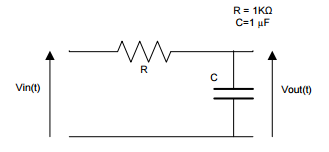
\includegraphics[width = 0.4\textwidth]{RC_filter}
    \caption{Single pole RC filter}
    \label{fig:RC_filter}
\end{figure}

The first step to converting the analogue filter to a digital one is to compute the transfer function of the analogue filter. This is presented in equation (\ref{eq:RC_transfer_function}). 

\begin{align}
    V_{out}(s)  &= \frac{1/sC}{R + 1/sC}V_{in}(s) \nonumber \\
                &= \frac{1}{1 + sRC}V_{in}(s) \nonumber \\
    H(s) &= \frac{V_{out}(s)}{V_{in}(s)} = \frac{1}{1 + sRC}\label{eq:RC_transfer_function}
\end{align}

It is clear that the filter is a low-pass filter. At low frequencies, $H(s) \approx 1$ while at high frequencies, $H(s) \approx 0$.\\

The next step is to apply the bilinear transformation, presented in equation (\ref{eq:bilinear_transform}) to the transfer function presented in equation (\ref{eq:RC_transfer_function}). This yields the transfer function of the digital filter. 

\begin{align}
    H(s)    &= \frac{1}{1 + (\frac{2}{T}\frac{z-1}{z+1})RC} \nonumber \\
            &= \frac{zT+T}{T(z+1) + 2(z-1)RC} \nonumber \\
            &= \frac{zT+T}{z(T+2RC) + (T-2RC)} \nonumber \\
            &= \frac{T+Tz^{-1}}{(T+2RC) + (T-2RC)z^{-1}} \\
            &= \frac{\frac{T}{T+2RC}+\frac{T}{T+2RC}z^{-1}}{1 + \frac{T-2RC}{T+2RC}z^{-1}}\label{eq:digital_RC_tf}
\end{align}

Equation (\ref{eq:digital_RC_tf}) shows the general form of a single pole analogue filter that has been mapped to the z-plane using the bilinear transformation. In laboratory 5, the values of R and C have been defined to be $1k\Omega$ and $1\mu F$ respectively; the sampling frequency is set to $8kHz$. These are substituted into equation (\ref{eq:digital_RC_tf}) and the final transfer function is presented in equation (\ref{eq:digital_RC_actual}).

\begin{align}
    H(z)    &= \frac{\frac{1}{17} + \frac{1}{17}z^{-1}}{1 - \frac{15}{17}z^{-1}}\label{eq:digital_RC_actual}
\end{align}

Finally, taking the inverse z-transform the difference equation presented in equation (\ref{eq:RC_diff_eq}) is obtained. 

\begin{align}
    y(n) &= \frac{1}{17}x(n) + \frac{1}{17}x(n-1) + \frac{15}{17}y(n-1) \label{eq:RC_diff_eq}
\end{align}

\textbf{As discussed in section \ref{sec:bilinear_transform}, the mapping from the analogue domain to the digital domain is non-linear. The effects of frequency warping were discussed and it was mentioned that the bilinear transformation will shift corner frequencies. The shifting of the corner frequencies can be compensated for when designing the analogue filter through a process referred to as pre-warping. This was however not considered when mapping the single-pole filter in figure \ref{fig:RC_filter} to the digital domain since the ratio of the corner frequency to the sampling frequency is small enough that the assumption $tan(\nicefrac{\Omega T}{2}) \approx \nicefrac{\Omega T}{2}$ is valid.} \\

To check the validity of the assumption, the analogue corner frequency is first calculated in equation (\ref{eq:analogue_corner_freq}).

\begin{align}
    \Omega_{c}  &= \frac{1}{RC}  = 1000 \ rad \nonumber \\
    F_{c}       &= 159.15Hz \label{eq:analogue_corner_freq}
\end{align}

Next, the digital corner frequency is computed using equation (\ref{eq:frequency_wrapping}). 

\begin{align}
    \omega_{c}  &= \frac{2}{T}tan^{-1}(\frac{\Omega_{c}T}{2}) = 998.70 \ rad \ s^{-1} \nonumber\\
    f_{c}       &= 158.94Hz\label{eq:digital_corner_freq}
\end{align}

\textbf{Equation (\ref{eq:digital_corner_freq}) shows that the assumption is valid and pre-warping does not have be applied in this case.} Figure \ref{fig:RC_ideal} shows the ideal frequency response of the RC filter once the bilinear transform has been applied and the analogue filter has been mapped to a digital filter.

\begin{figure}[H]
    \centering
    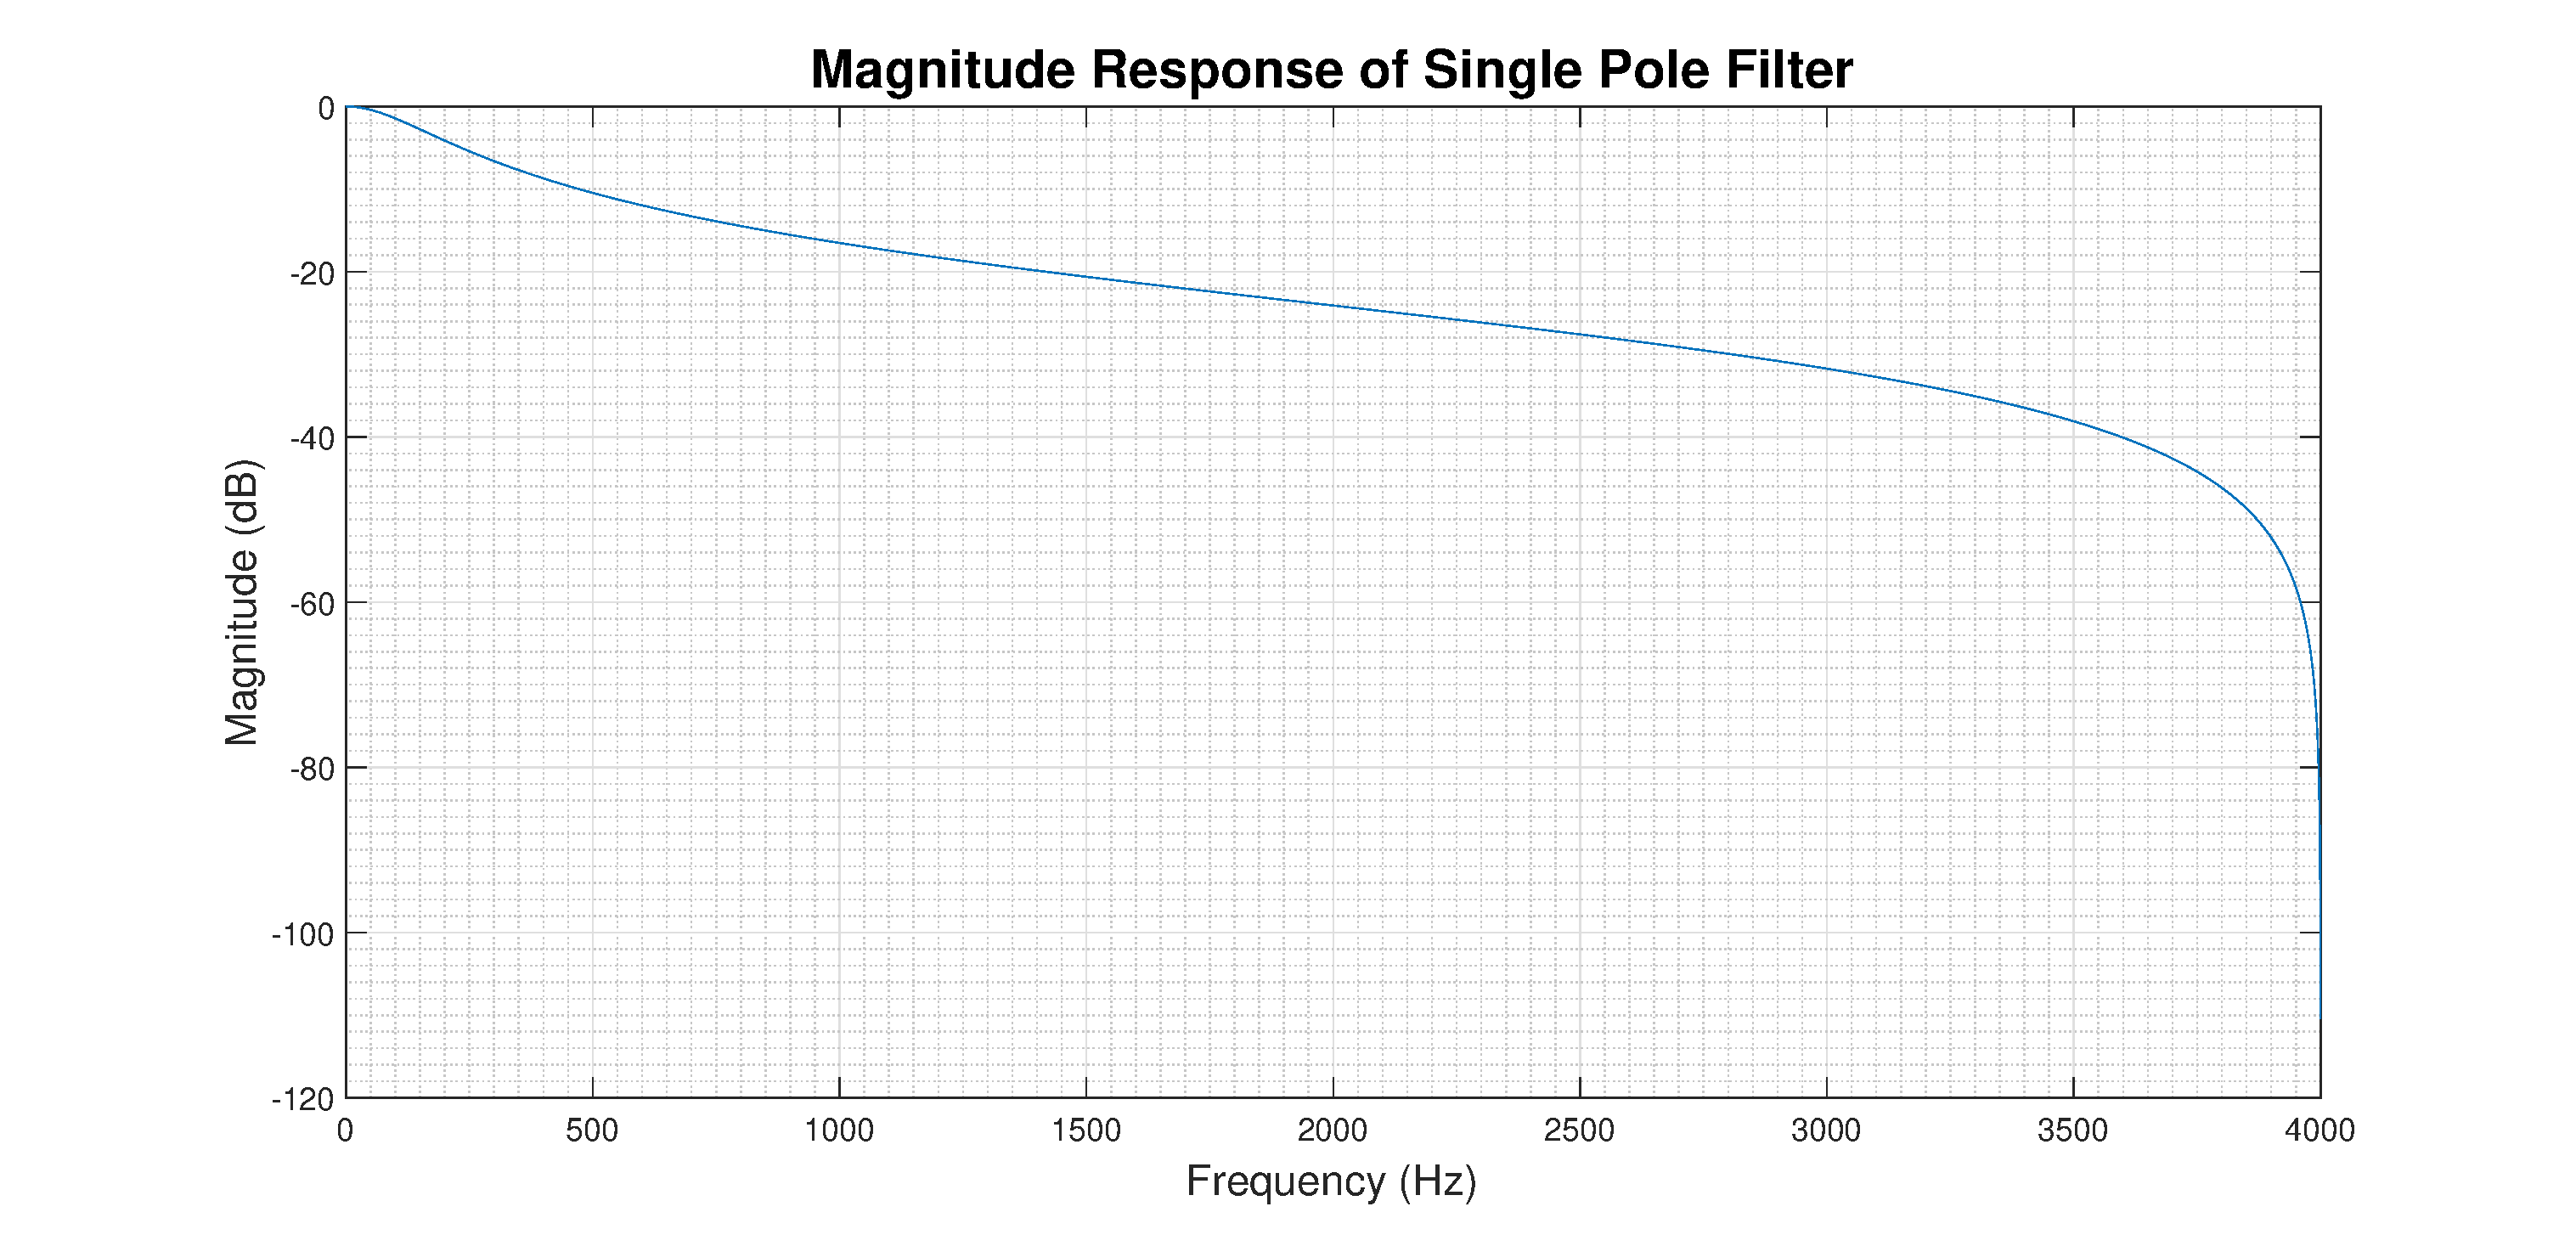
\includegraphics[width = 0.49\textwidth]{mag_response_ideal}
    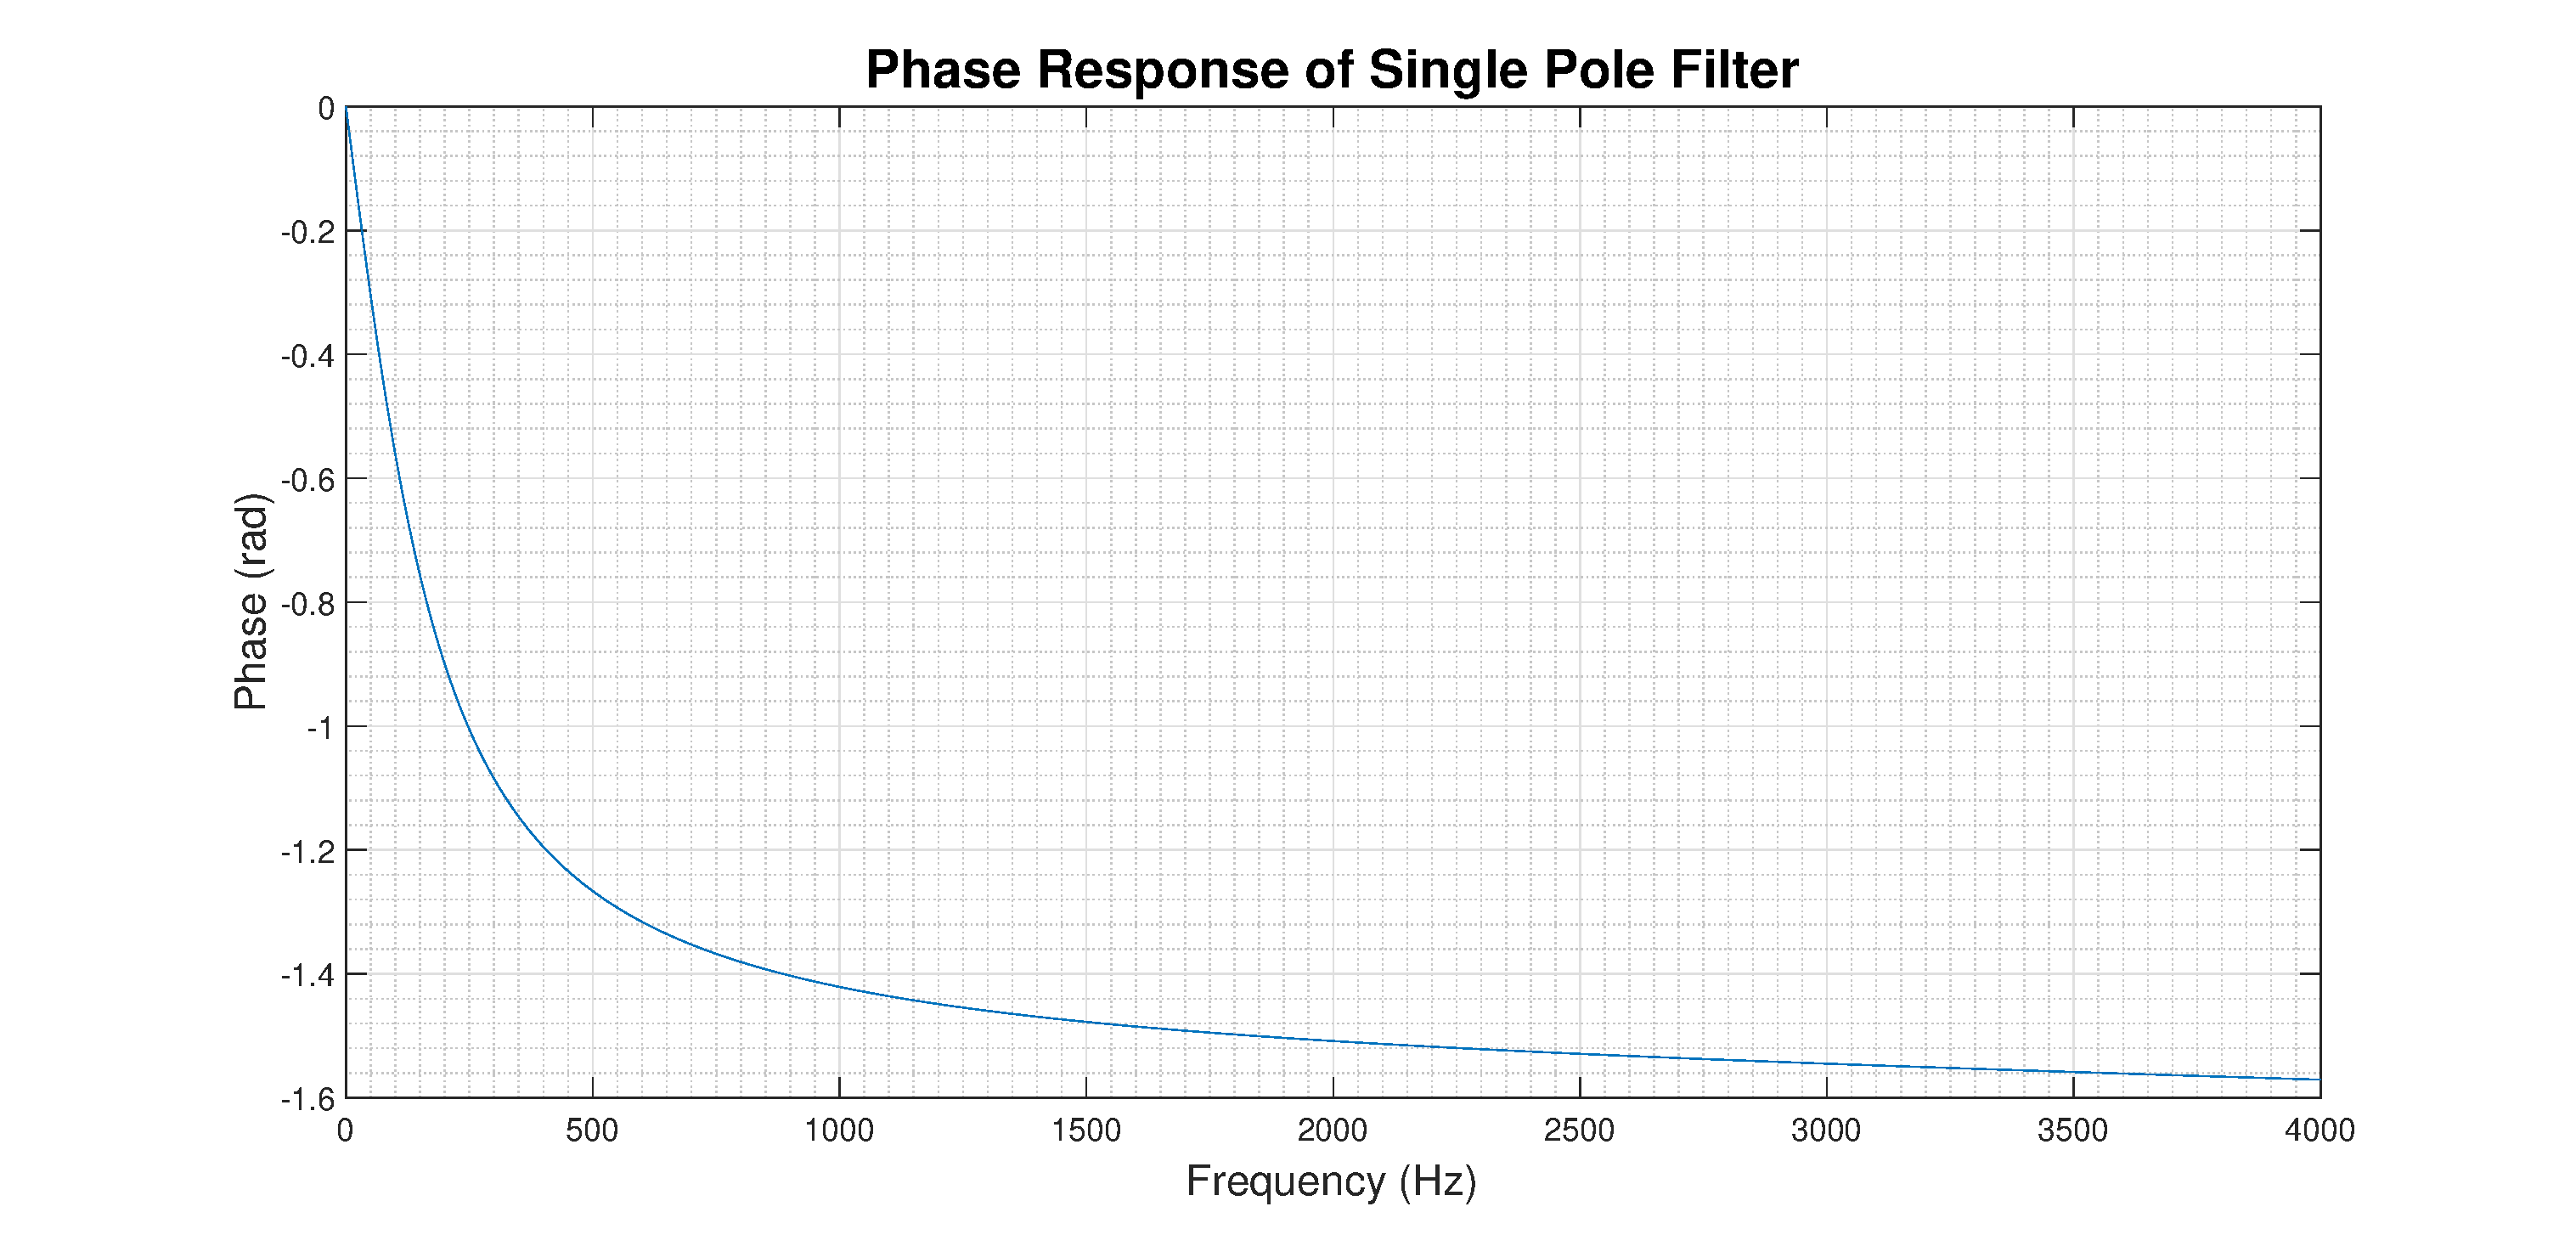
\includegraphics[width = 0.49\textwidth]{phase_response_ideal}
    \caption{Ideal frequency response of the designed filter}
    \label{fig:RC_ideal}
\end{figure}

\textbf{Figure \ref{fig:RC_corner_ideal} shows that the corner frequency of the digital filter is indeed at $158Hz$.}

\begin{figure}[H]
    \centering
    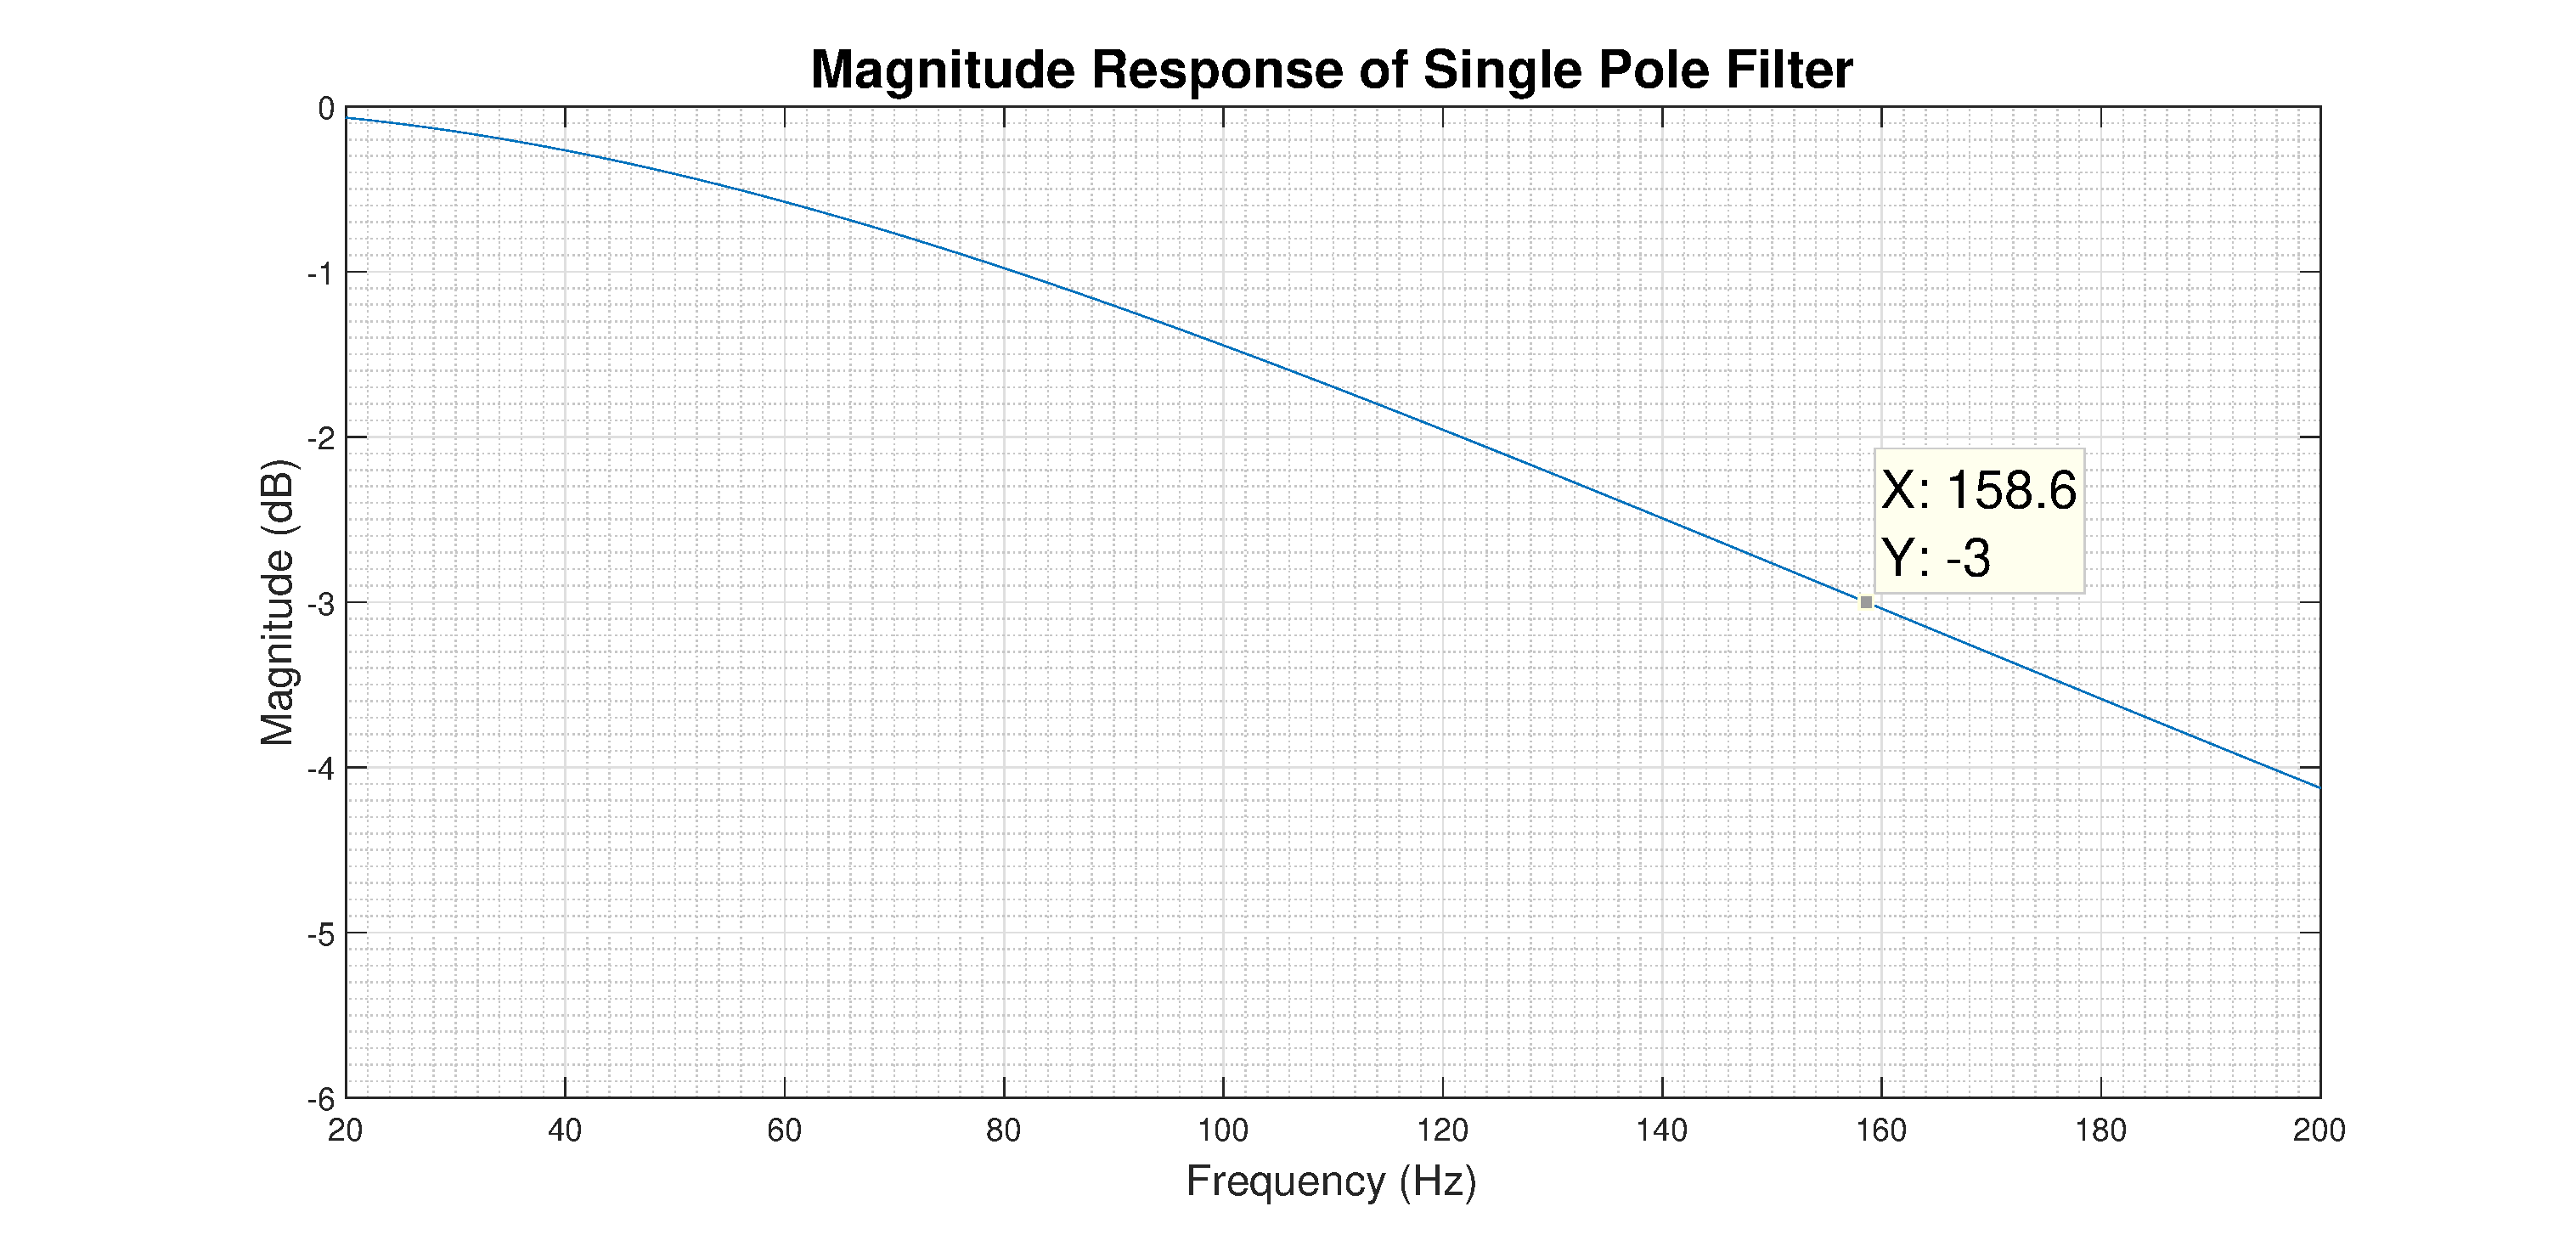
\includegraphics[width = 0.70\textwidth]{time_constant_ideal}
    \caption{Ideal frequency response of the designed filter}
    \label{fig:RC_corner_ideal}
\end{figure}

\newpage
\subsection{Ideal corner frequency of digital filter}

In section \ref{sec:design_of_digital_filter}, the bilinear transform was utilised to convert a single pole analogue filter into a digital filter. The filter was presented in equation (\ref{eq:RC_diff_eq}) in the form of a difference equation. To implement the digital filter on the $TMS320C6713 \ DSK$ board, the code presented in listing \ref{lst:single_pole} was used.

\begin{listing}[H]
\begin{minted}[fontsize=\scriptsize,linenos]{C}
// defining filter coefficients and 
// initialising variables to hold inputs and outputs
// as global variables
const double a = 0.8823529411764706;
const double b = 0.05882352941176471;
double x[2] = {0}; 
double y = 0;

void ISR_filter(void){
    // reading of new sample
    x[0] = mono_read_16Bit();
    
    // output of filter is calculated using RC_filter function
    y = RC_filter();
    
    // calculated output written to audio codec
    mono_write_16Bit((short)y);
}

double RC_filter(void){			
    // output is computed in accordance with filter's difference equation
    y = b*(x[0] + x[1]) + a*y;
    
    // position of buffer is updated
    x[1] = x[0];
    
    return(output);		
}
\end{minted}
\caption{C code to implement single pole digital filter} 
\label{lst:single_pole}
\end{listing}

The code required to implement the single pole filter is extremely simple. The order of the filter is 1 thus only 3 elements need to be stored. The array of doubles, x, needed to store previous inputs, is defined as a global variable of size 2; both elements in the array are initialised to 0. Observing the form of the equation (\ref{eq:RC_diff_eq}), it is clear that the variable y, which is used to store the current output can be reused when calculating the next output.\\

As in the laboratory 4, the filter coefficients are stored as double-precision floating point numbers. As discussed in section \ref{sec:IIR_filter}, the digital representation of numbers may result in poles drifting out of the unit circle. This should be carefully considered as implementing the filter designed in section \ref{sec:design_of_digital_filter} requires representing the filter coefficients, calculated to be fractions, as double-precision floating point numbers. \textbf{In this case however, the error incurred does not result in instability as the pole is located a significant distance away from the unit circle\footnote{Higher order filters are more suspectile to rounding errors.}.}\\ 

Each time a new sample is read, the samples within the buffer are rearranged such that the index of the array represents the relative delay between the current sample and the stored sample. In laboratory 4, this structure was referred to as a simple non circular buffer\textbf{. The overhead for rearranging elements was significant in the previous laboratory session because the number of filter coefficients was in excess of 200. In this case however, a simple buffer does not require much computation complexity to be maintained.} \\

The output of the filtering process is performed with just $1$ line of code. This is again possible because the number of filter coefficients is extremely small.

\subsection{Verification of Time Constant}\label{sec:time_const}

An important design parameters in the design of analogue filter is the time constant. The time constant for the analogue filter presented in figure \ref{fig:RC_filter} is calculated in equation (\ref{eq:RC_time_constant}).

\begin{align}
    \tau_{a} = RC = 1.000ms\label{eq:RC_time_constant}
\end{align}

Notice that the time constant is the inverse of the corner frequency, scaled by $2\pi$, which was calculated in equation (\ref{eq:analogue_corner_freq}). The frequency warping introduced due to the non-linear nature of the bilinear transform will slightly change the time constant of the digital filter. Equation (\ref{eq:time_constant_digital_ideal}) shows the time constant of the digital filter. It is calculated using the corner frequency stated in equation (\ref{eq:digital_corner_freq}).

\begin{align}
    \tau_{d} = \frac{1}{2\pi (158.94)}= 1.001ms\label{eq:time_constant_digital_ideal}
\end{align}

\textbf{To verify that the time constant for the digital filter matches the theoretical value of $1.001ms$, a square wave is used as an input to the filter.} The external connections of the $AIC23$ audio codec, presented in figure \ref{fig:AIC23_audio_codec}, show the presence of a high-pass filter at the input. 

\begin{figure}[H]
\centering
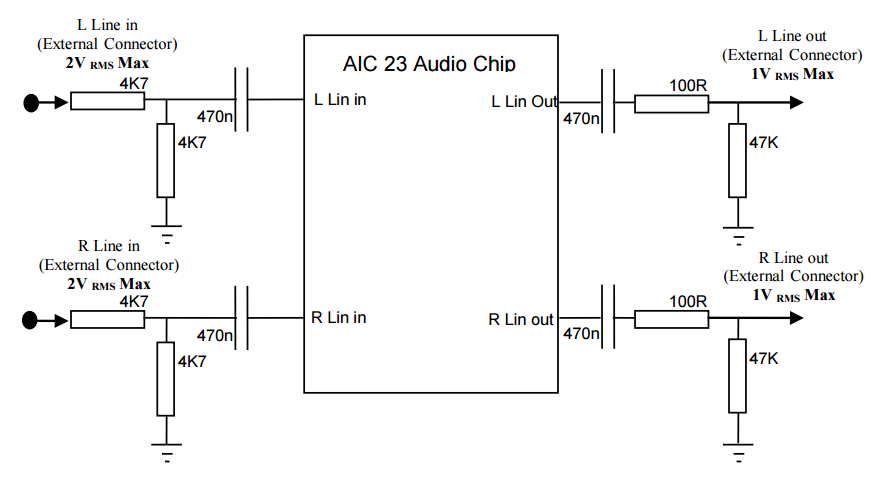
\includegraphics[width=0.4\textwidth]{AIC23.PNG}
\caption{AIC23 audio chip external connections\cite{AIC23_technical_reference}}
\label{fig:AIC23_audio_codec}
\end{figure}

The high-pass filter has the following transfer function, where $R_{1}=100 \Omega$, $R_{2}=47 k\Omega$ and $C=470nF$:

\begin{equation}
    H(s)=\frac{V_o(s)}{V_{i}(s)} = \frac{R_{2}Cs}{1 + (R_{1}+R_{2})Cs}   
\end{equation}

The corner frequency of the filter is:

\begin{equation}
     f_p = \frac{1}{2\pi (R_1+R_2)C} = \frac{1}{2\pi (100 + 47\cdot 10^{3})(470\cdot 10^{-9})} = 7.1895Hz
\end{equation}

\textbf{To avoid distortion from the high-pass filters on the $AIC23$ audio codec, a square wave of frequency $150Hz$ is used as an input.} The oscilloscope traces obtained are presented in figure \ref{fig:scope_RC}.

\begin{figure}[H]
\centering
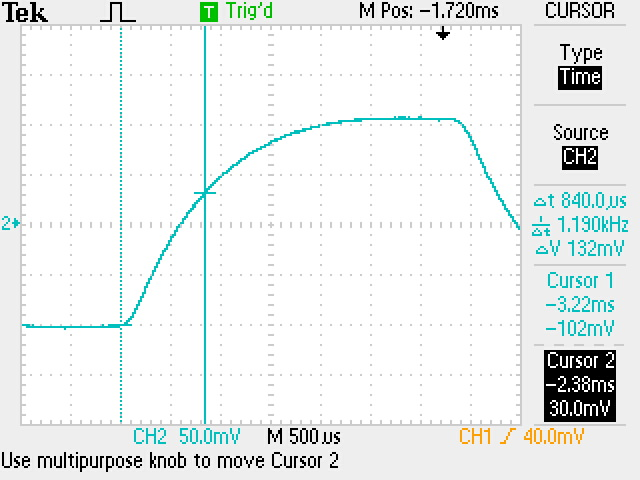
\includegraphics[width=0.49\textwidth]{RC_rising}
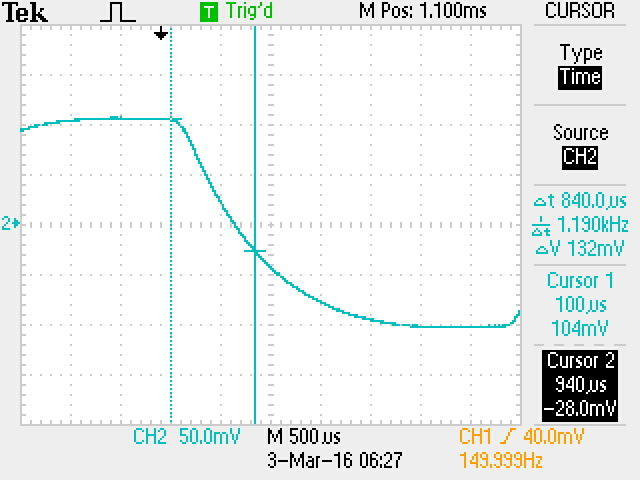
\includegraphics[width=0.49\textwidth]{RC_falling}
\caption{Oscilloscpoe traces used for calculation of time constant of digital filter}
\label{fig:scope_RC}
\end{figure}

The time constant of the circuit physically represents the time taken for the system's step response to reach $63.2\%$. The peak-to-peak voltage of the output wave is $220mV$ and thus a voltage change of $132mV$ is equivalent to  a $63.2\%$ increase/decrease.\\

\textbf{From figure \ref{fig:scope_RC}, it is clear that the time constant of the digital filter is $0.840ms$. This is slightly off from theoretical value of the digital filter of $1.001ms$.}\\

\textbf{Note that the frequency of $150Hz$ is perfect to measure the time constant of the digital filter. A square wave of a lower frequency would be distorted due to the high-pass nature of the filters connected to the $AIC23$ audio codec. A square wave of a higher frequency would not allow the output of the digital filter to settle close to its asymptotic value. In the analogue domain, this is equivalent to the capacitor not charging or discharging fully. Using an input square wave of $150Hz$ provides more than enough time\footnote{A frequency of $150Hz$ corresponds to a period of $6.66ms$. This is greater than 5 time constants than thus the output should have settled to within $99\%$ of its asymptotic value.} for the output to settle to very near its asymptotic value.} This is shown in figure \ref{fig:high_frequency_input}.

\begin{figure}[H]
    \centering
    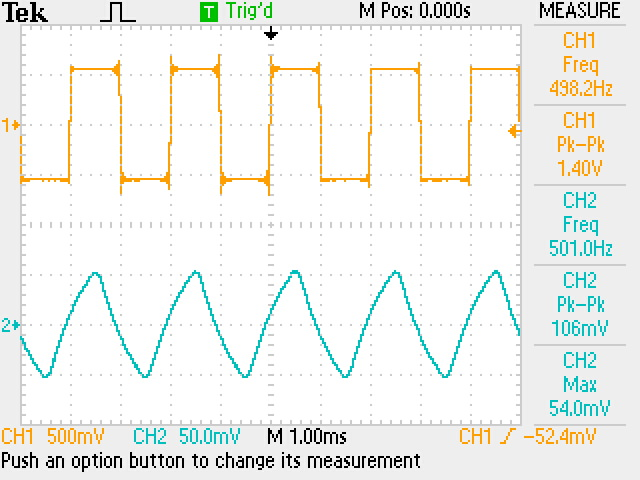
\includegraphics{Clipping}
    \caption{Oscilloscope trace when a high frequency square wave is used as an input}
    \label{fig:high_frequency_input}
\end{figure}

\subsection{Frequency Response}\label{sec:RC_freq}
Before the frequency response of the designed single pole filter can be studied, it is important to realise that the $TMS320C6713 \ DSK$ will have a non-flat frequency response even if no filtering is applied. This is due to the 2 analogue filter, 2 digital filters and multiple network of resistors that are present on the board. For accurate analysis, the frequency response of the $DSK$  board has to be taken into account. Figure \ref{fig:dsk_response} shows the response of the $DSK$  board.

\begin{figure}[H]
    \centering
    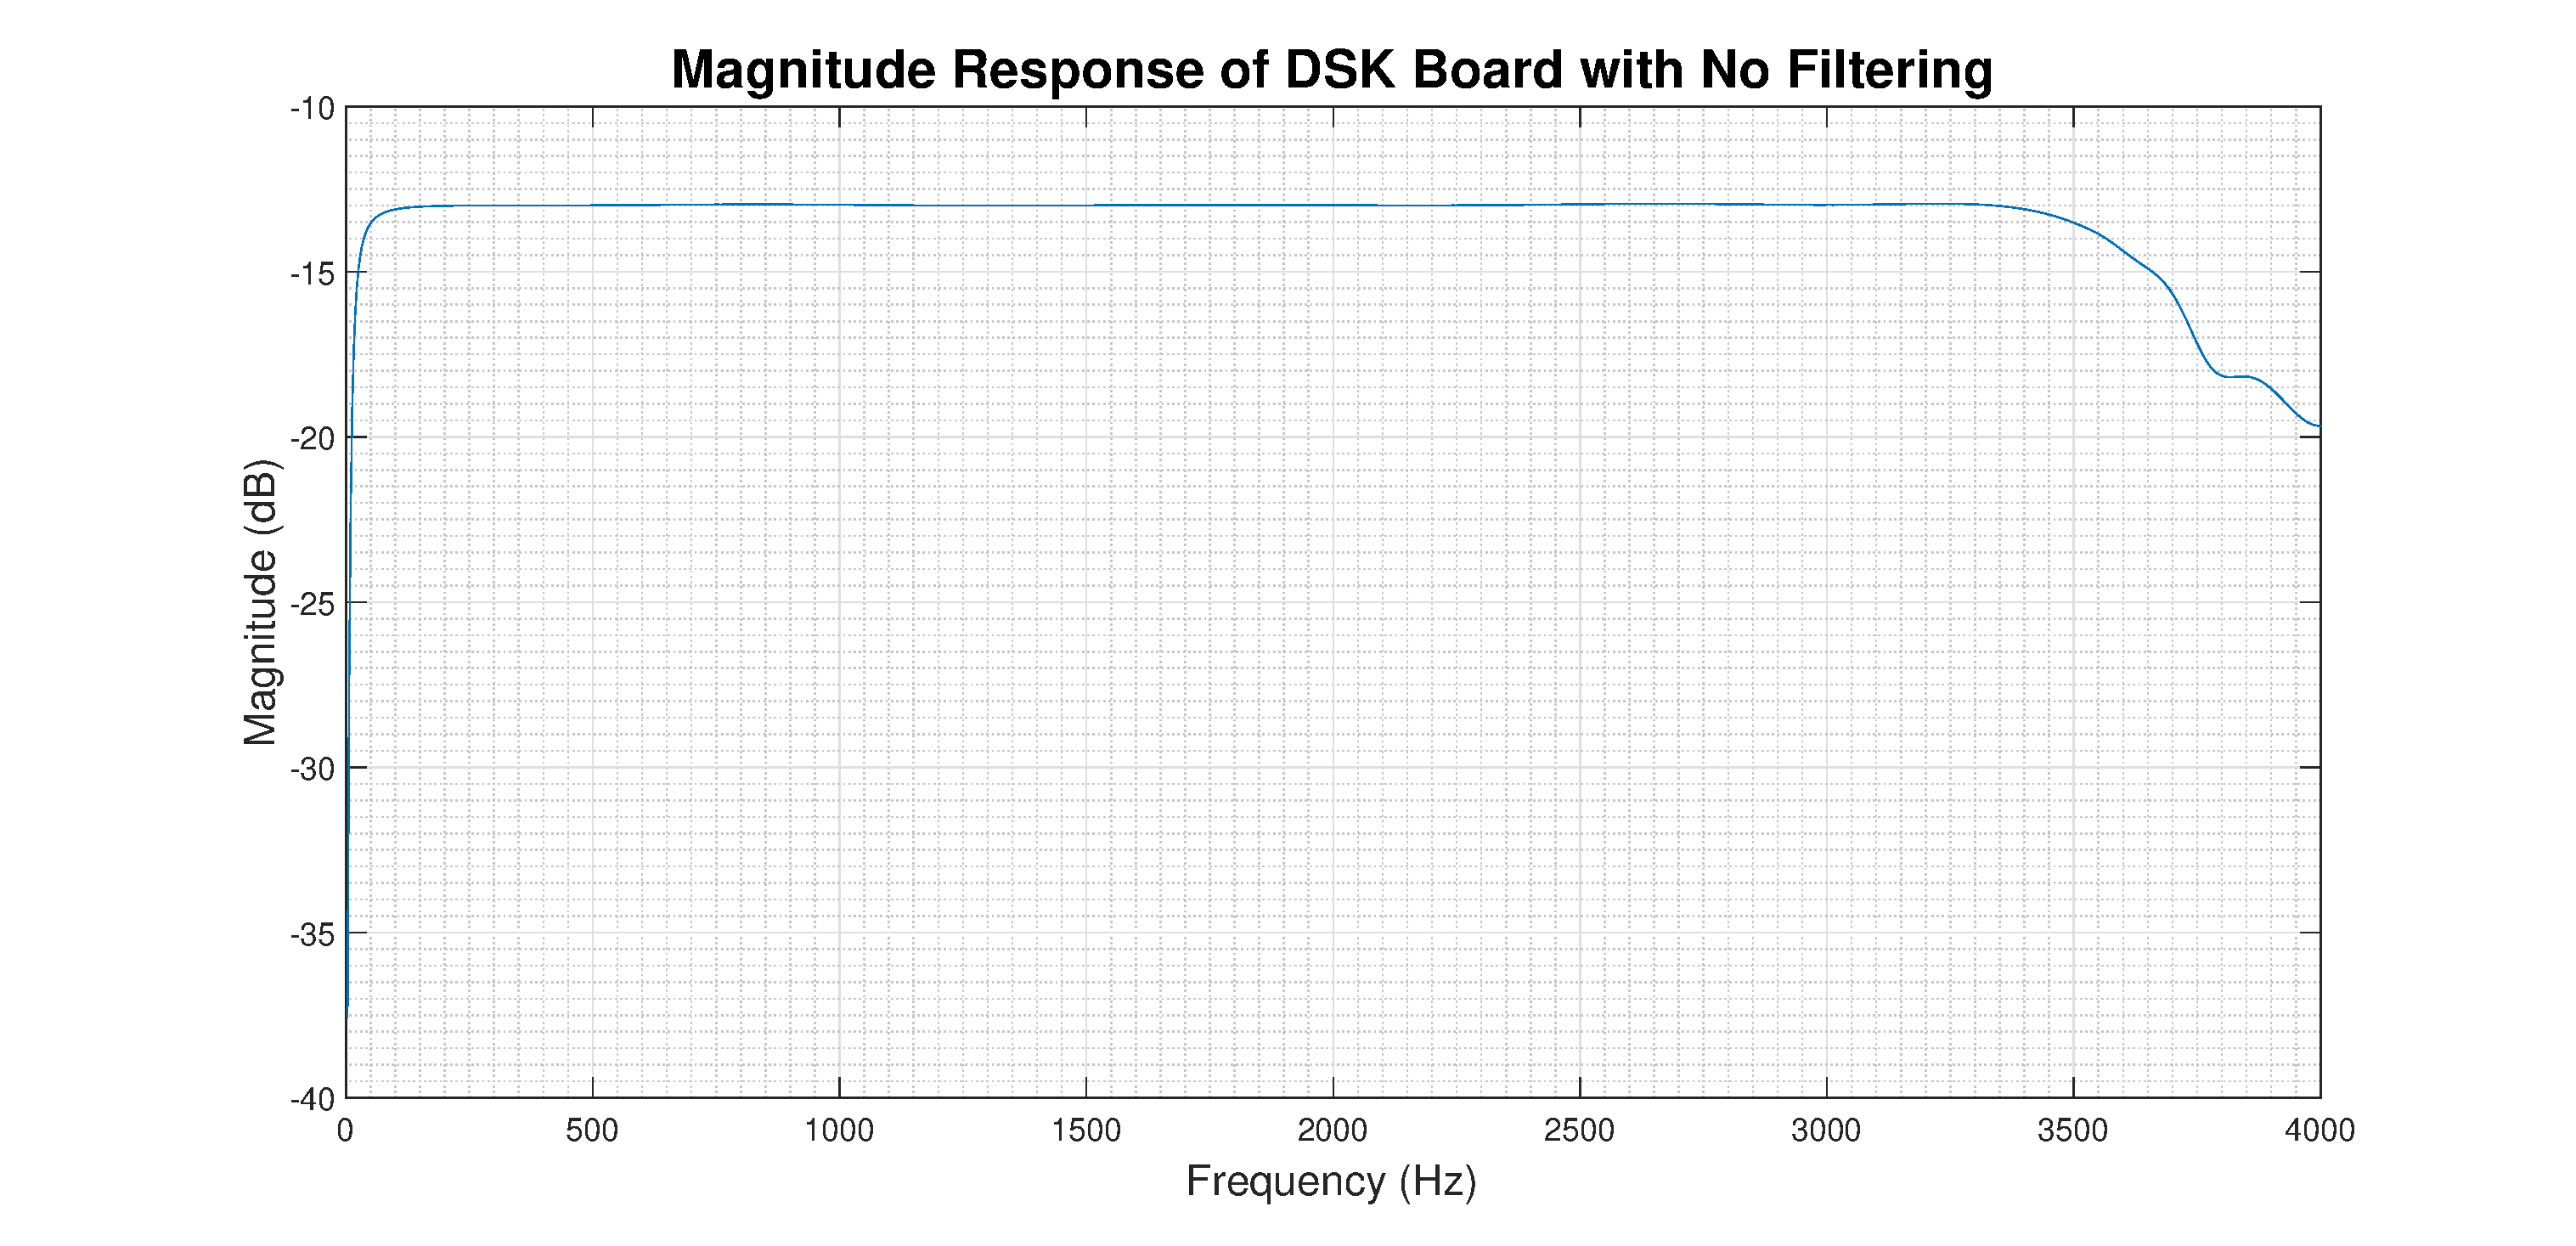
\includegraphics[width=0.49\textwidth]{mag_response_dsk}
    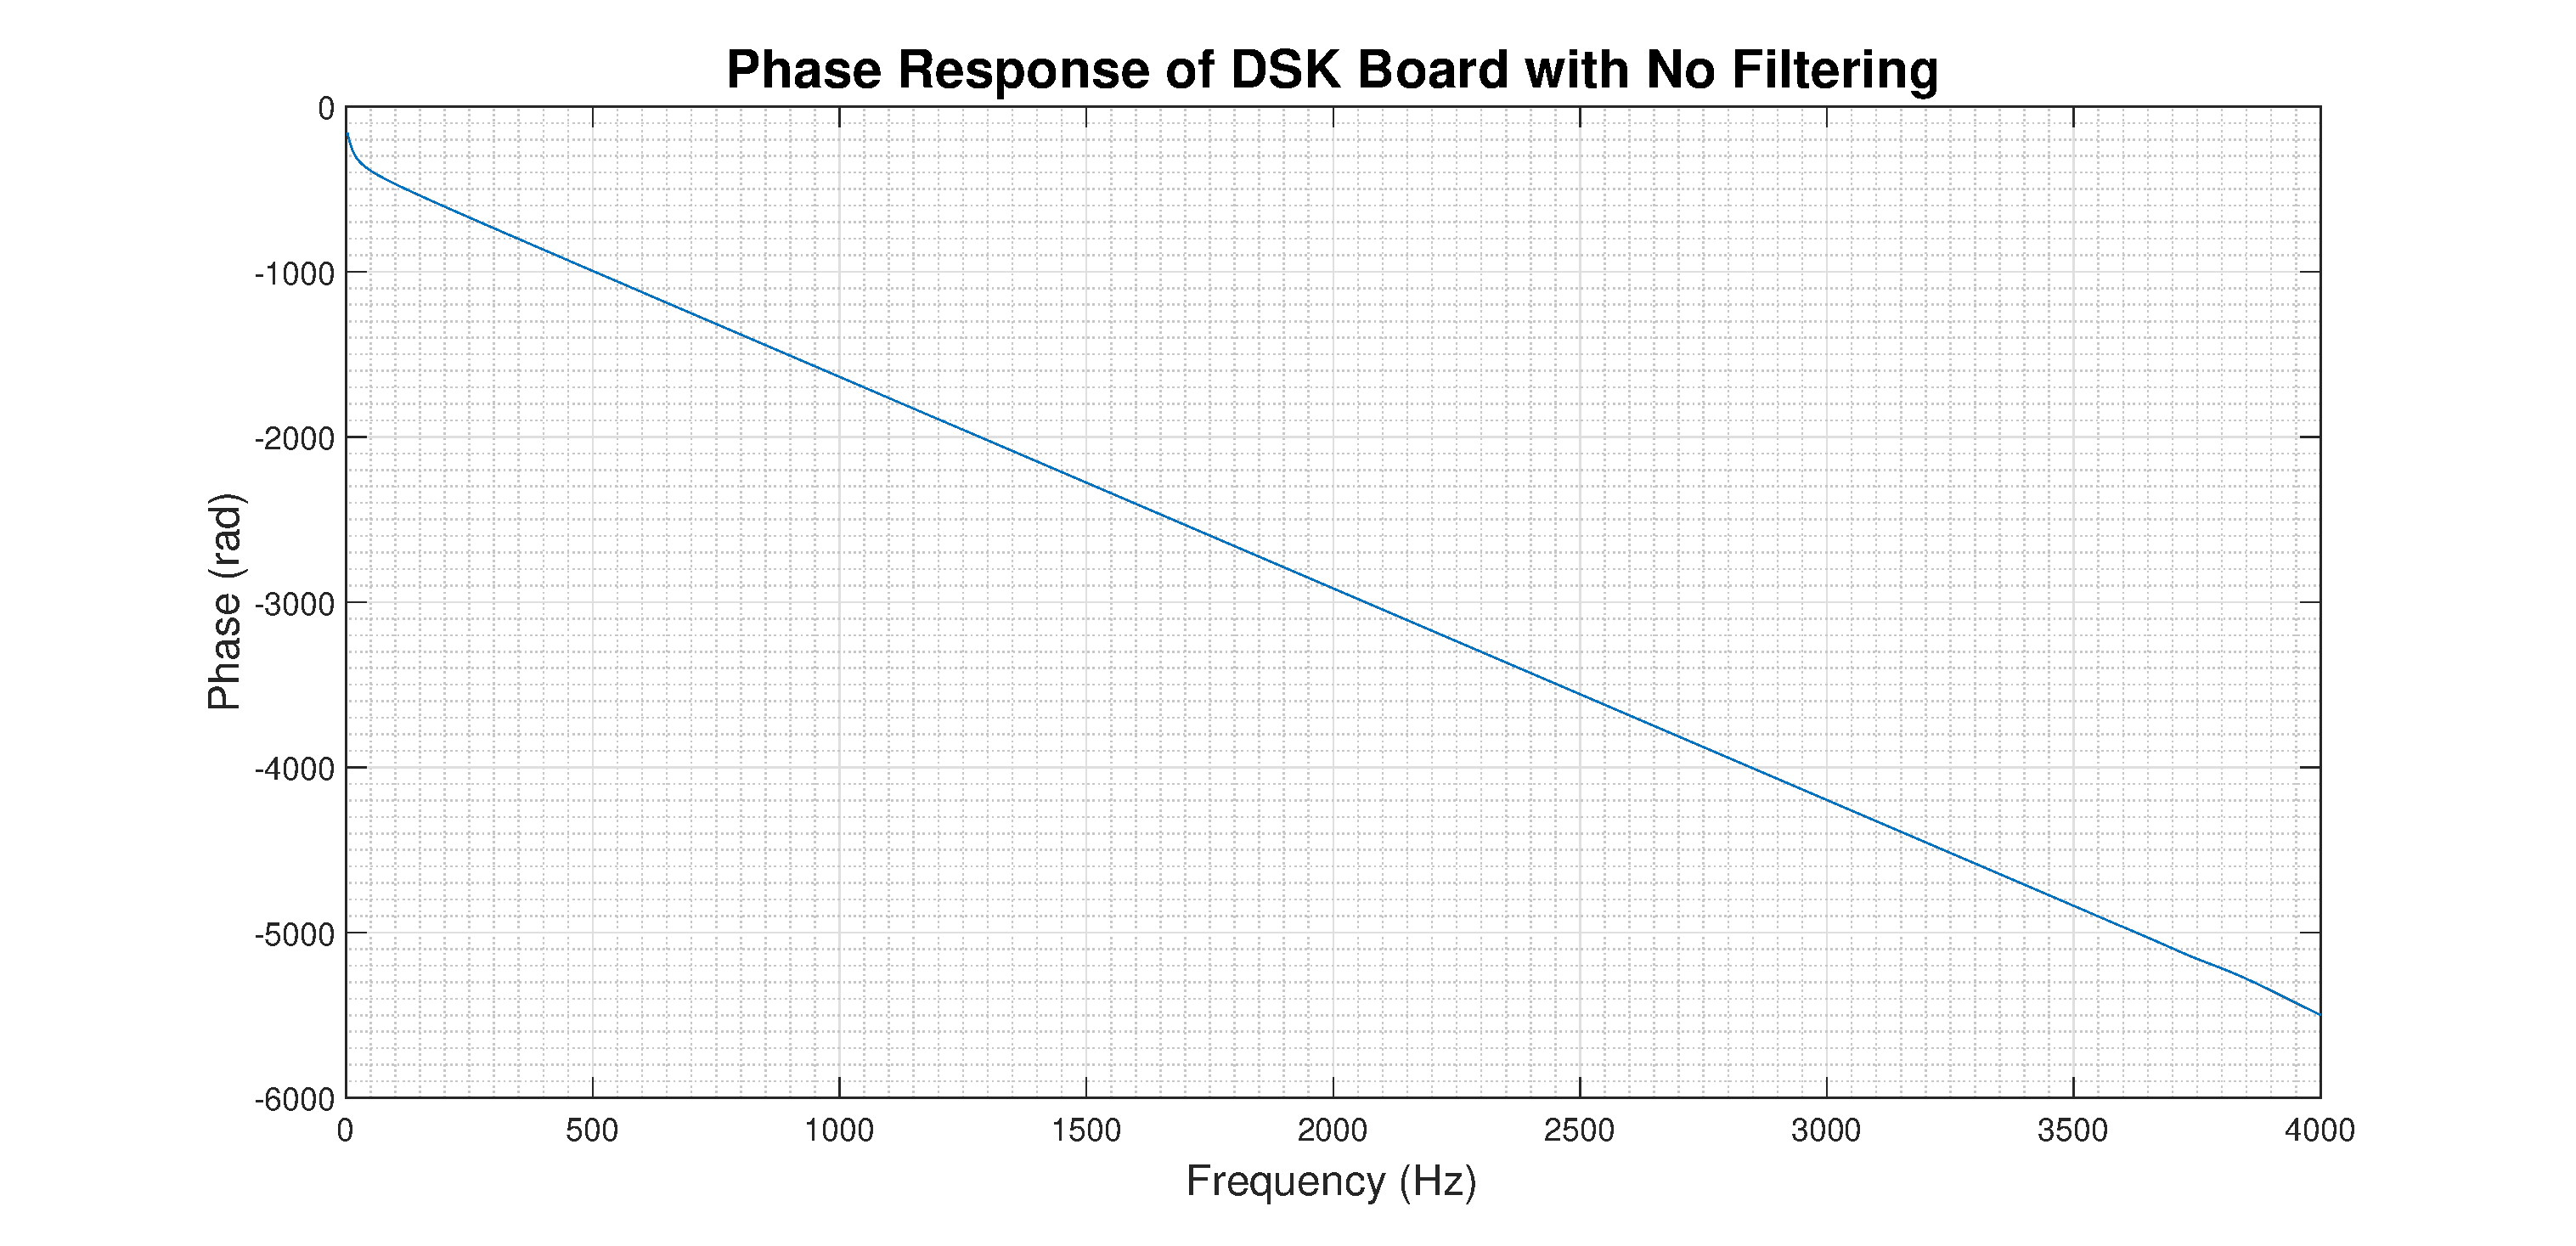
\includegraphics[width=0.49\textwidth]{phase_response_dsk}
    \caption{Frequency response of $TMS320C6713 \ DSK$ board without any filter}
    \label{fig:dsk_response}
\end{figure}

Pass band gain of $-12dB$ corresponds to a gain of approximately $\nicefrac{1}{4}$. This is exactly as expected.  

Next, figure \ref{fig:old_filter} shows the frequency response of the filter designed in section \ref{sec:design_of_digital_filter}. Note that the magnitude response in the pass band is centred about $-12dB$. This is discrepancy comes about because of the inherent frequency response of the $DSK$ board as discussed above. 

\begin{figure}[H]
    \centering
    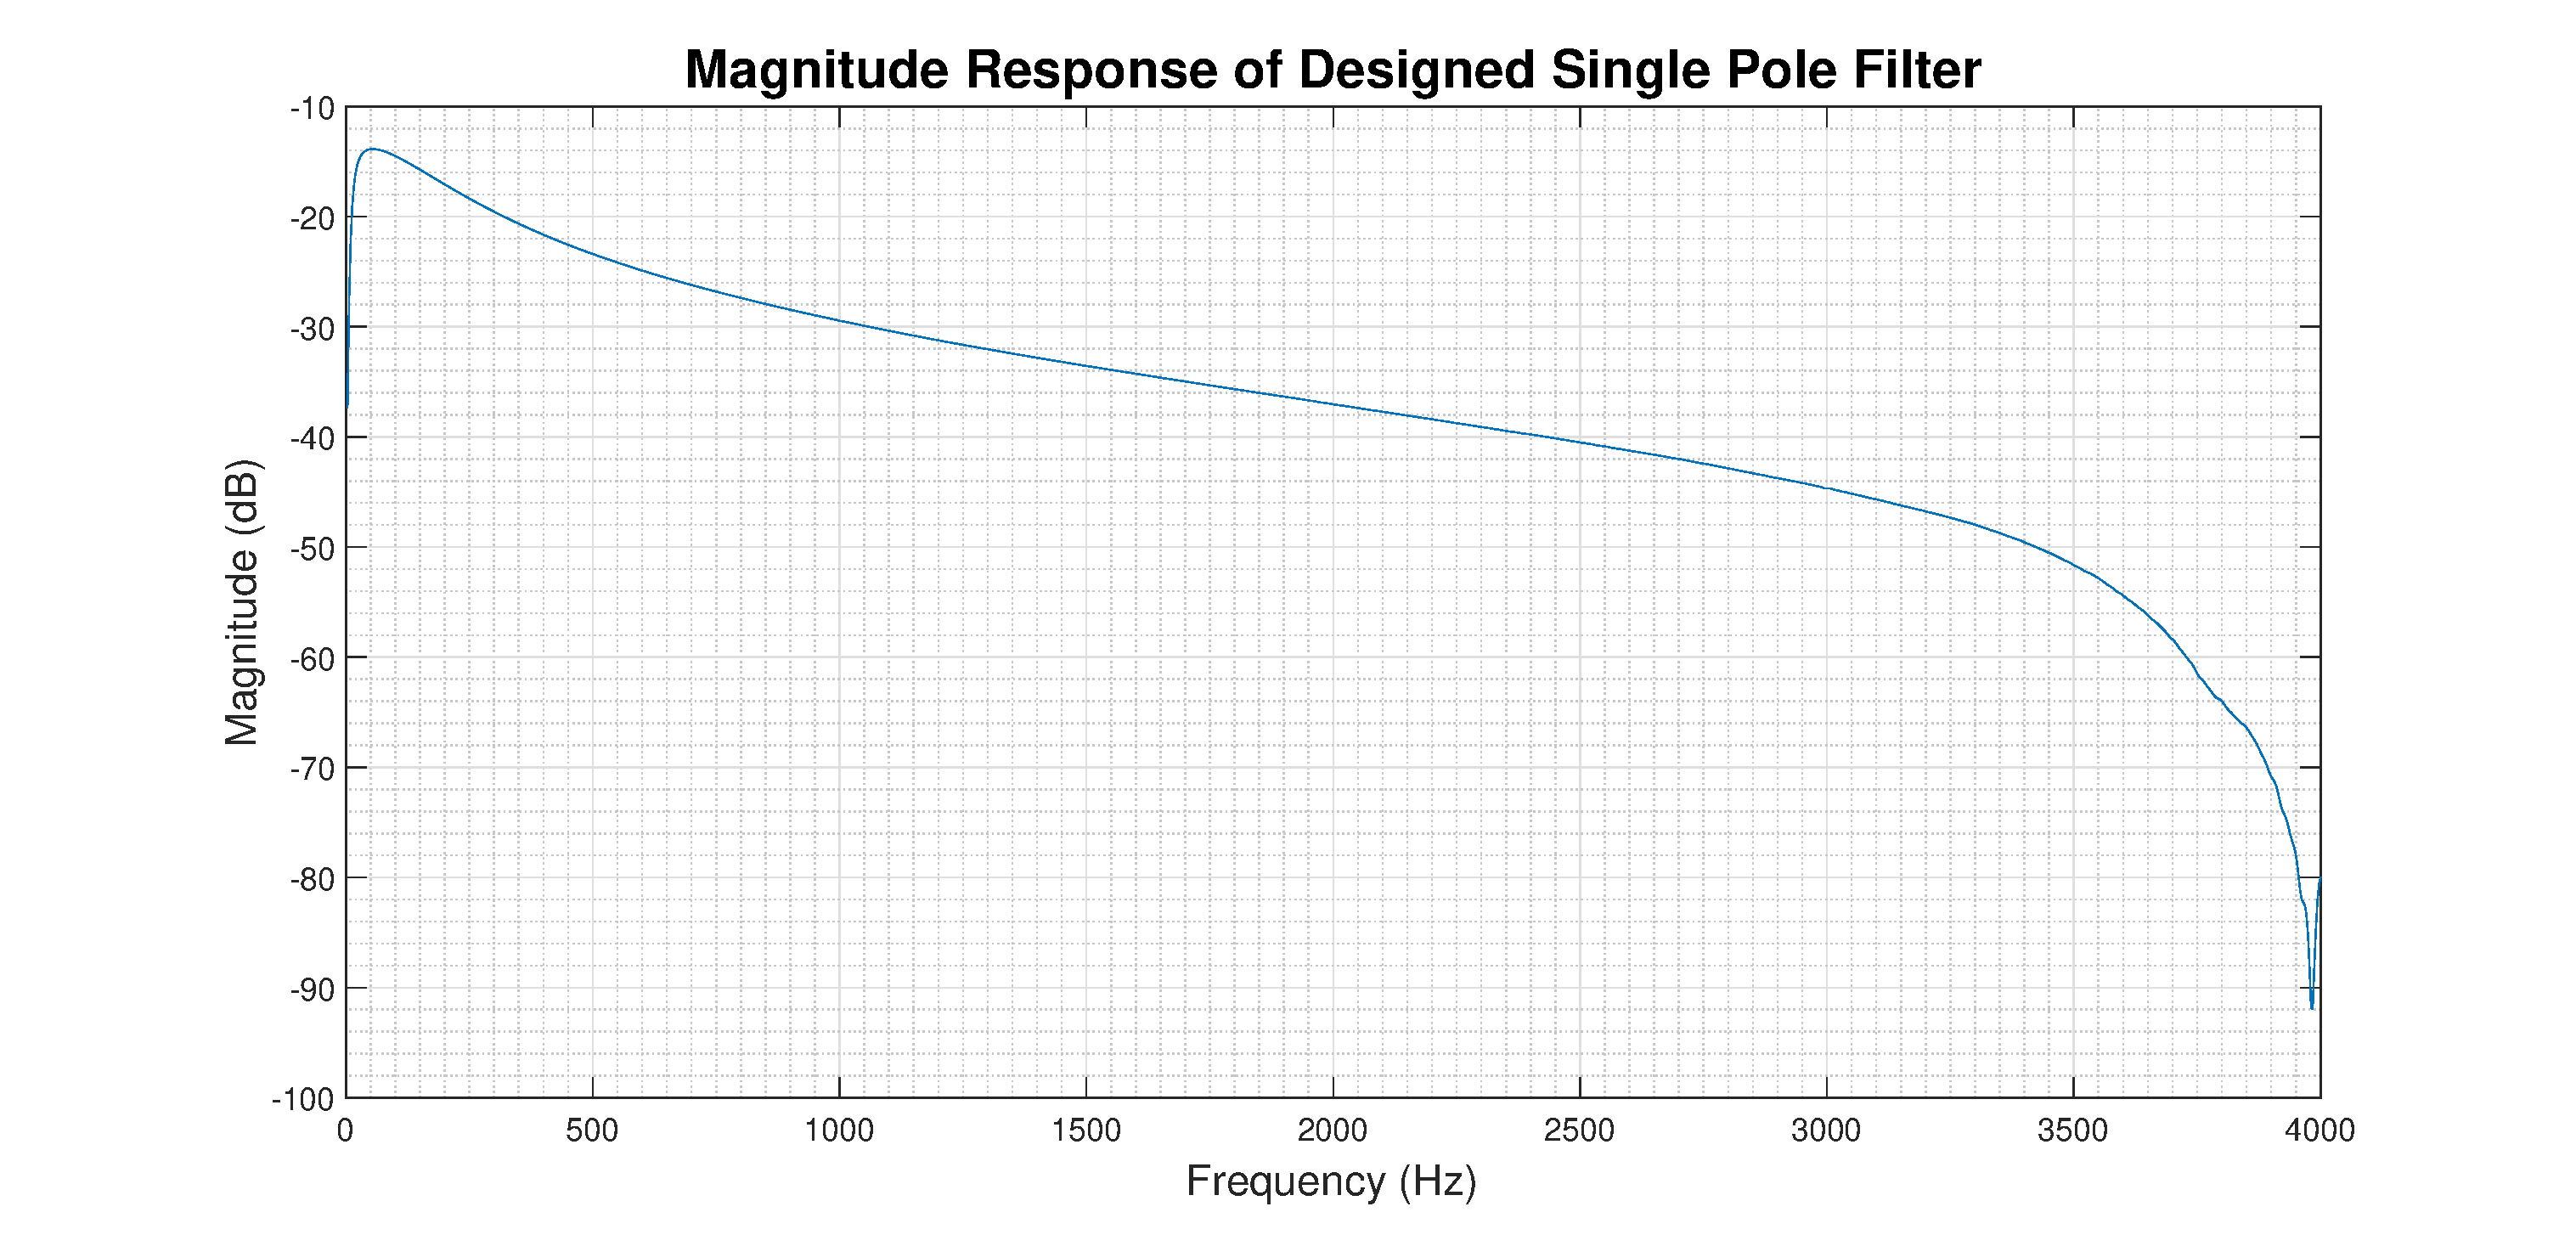
\includegraphics[width=0.49\textwidth]{mag_response_designed_single_pole_filter}
    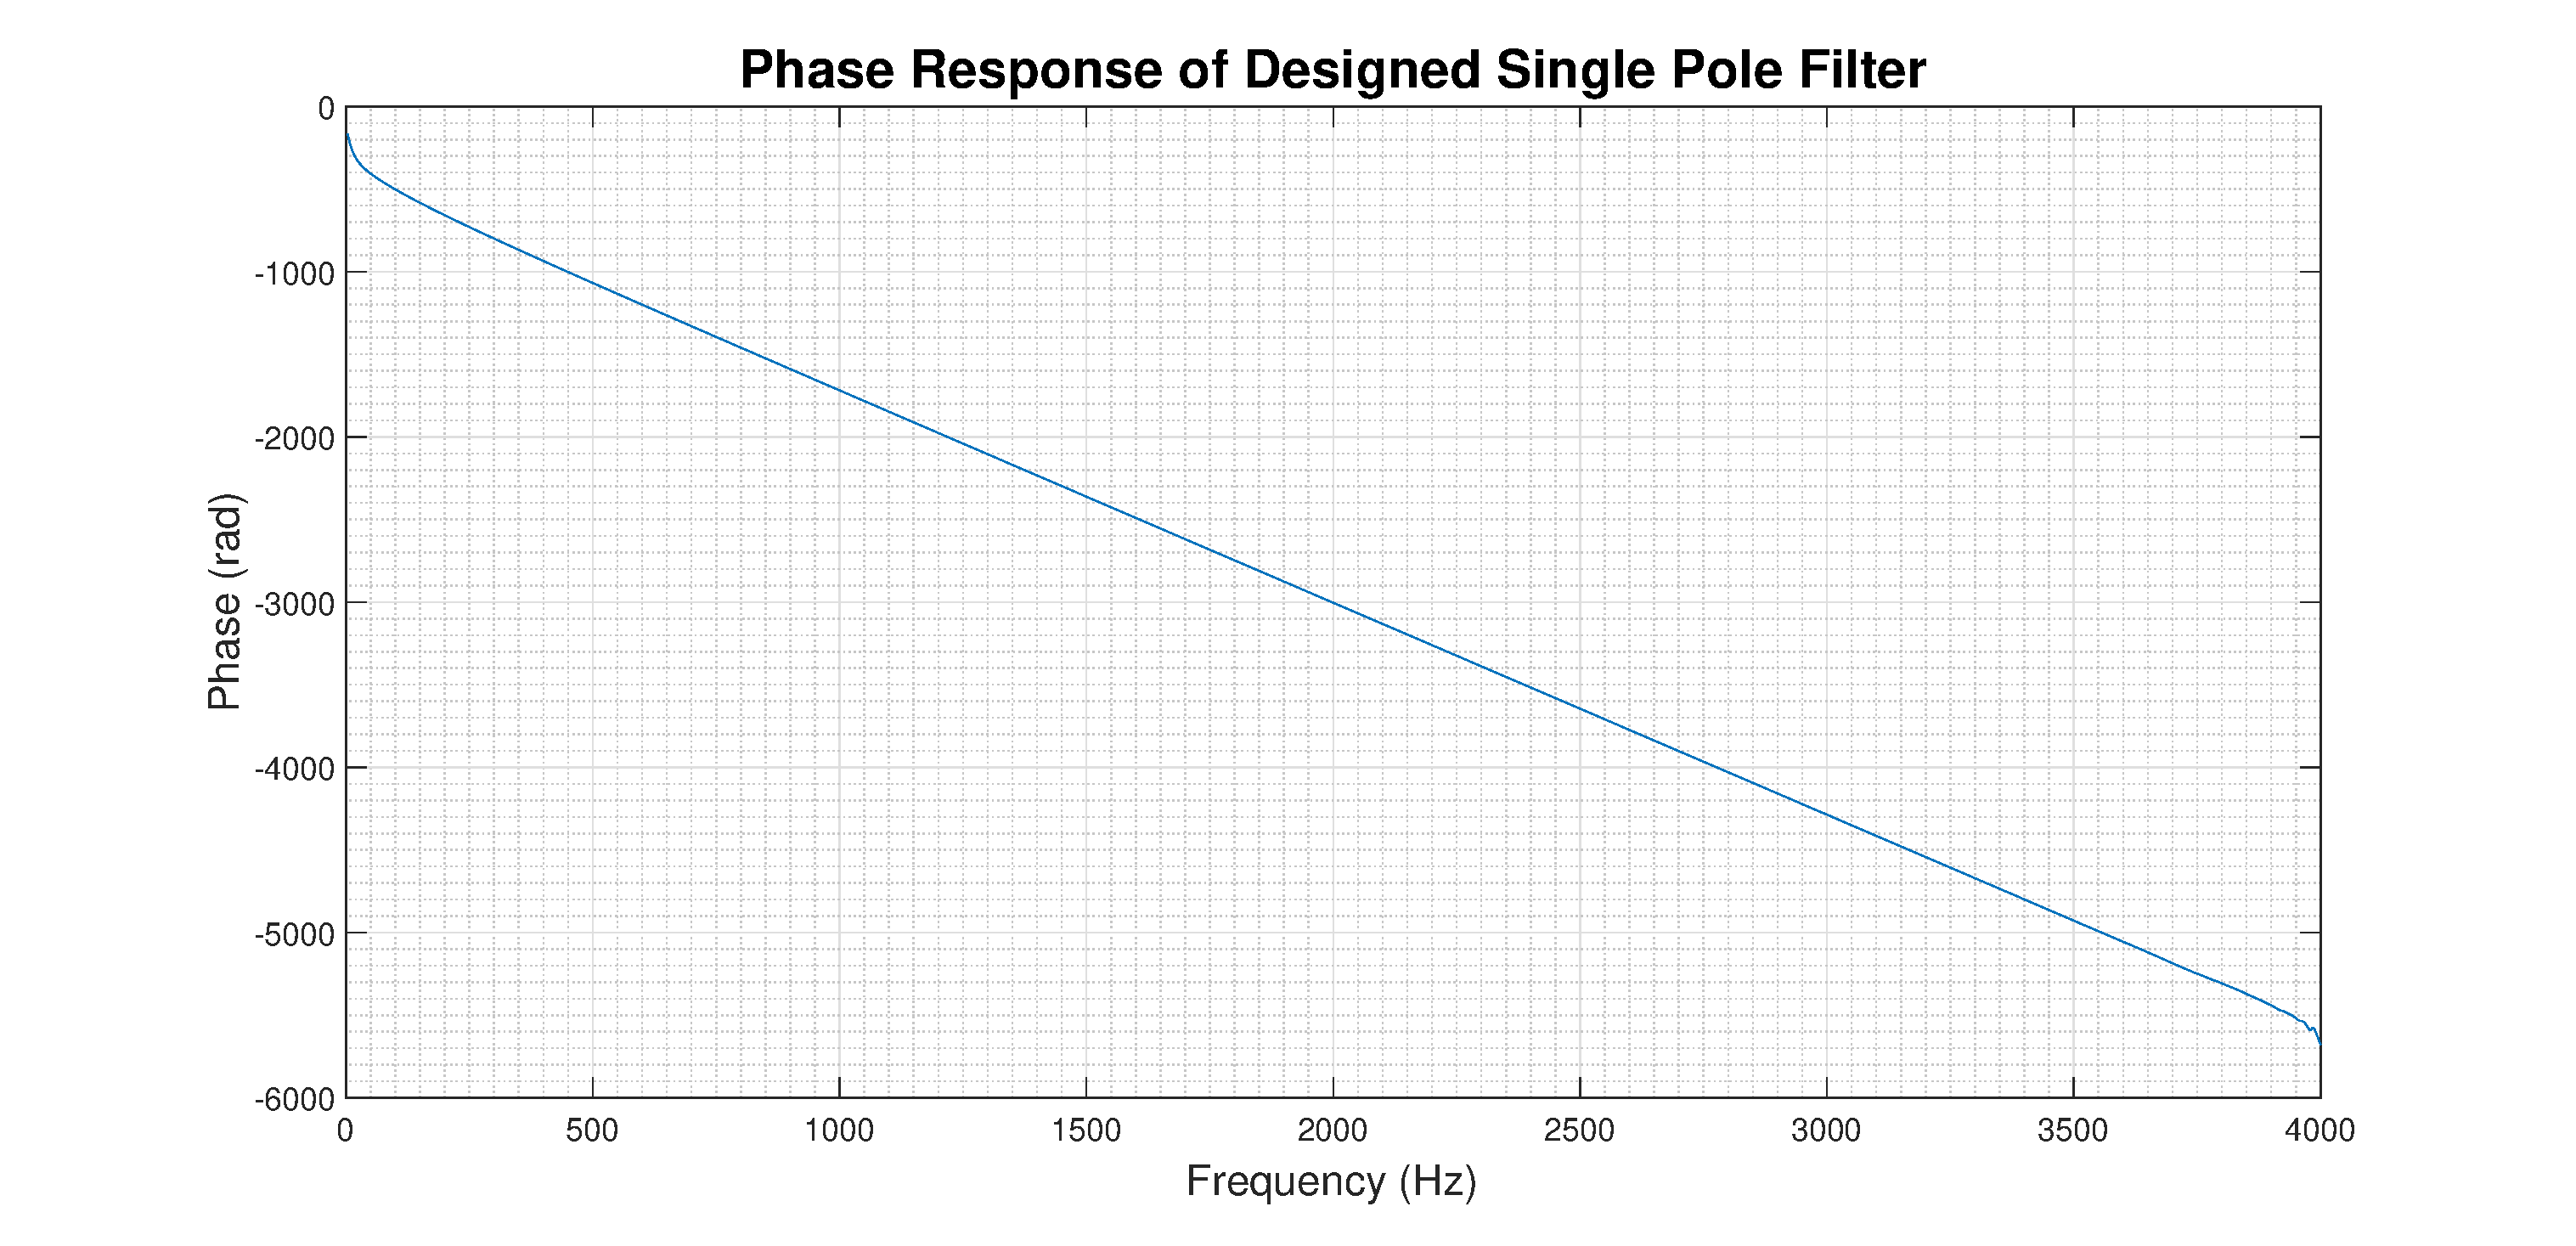
\includegraphics[width=0.49\textwidth]{phase_response_designed_single_pole_filter}
    \caption{Frequency response of the filter designed in section \ref{sec:design_of_digital_filter}}
    \label{fig:old_filter}
\end{figure}

Finally, figure \ref{fig:old_filter_subtracted} shows the frequency response once the offset introduced by the $DSK$ board is taken into account.

\begin{figure}[H]
    \centering
    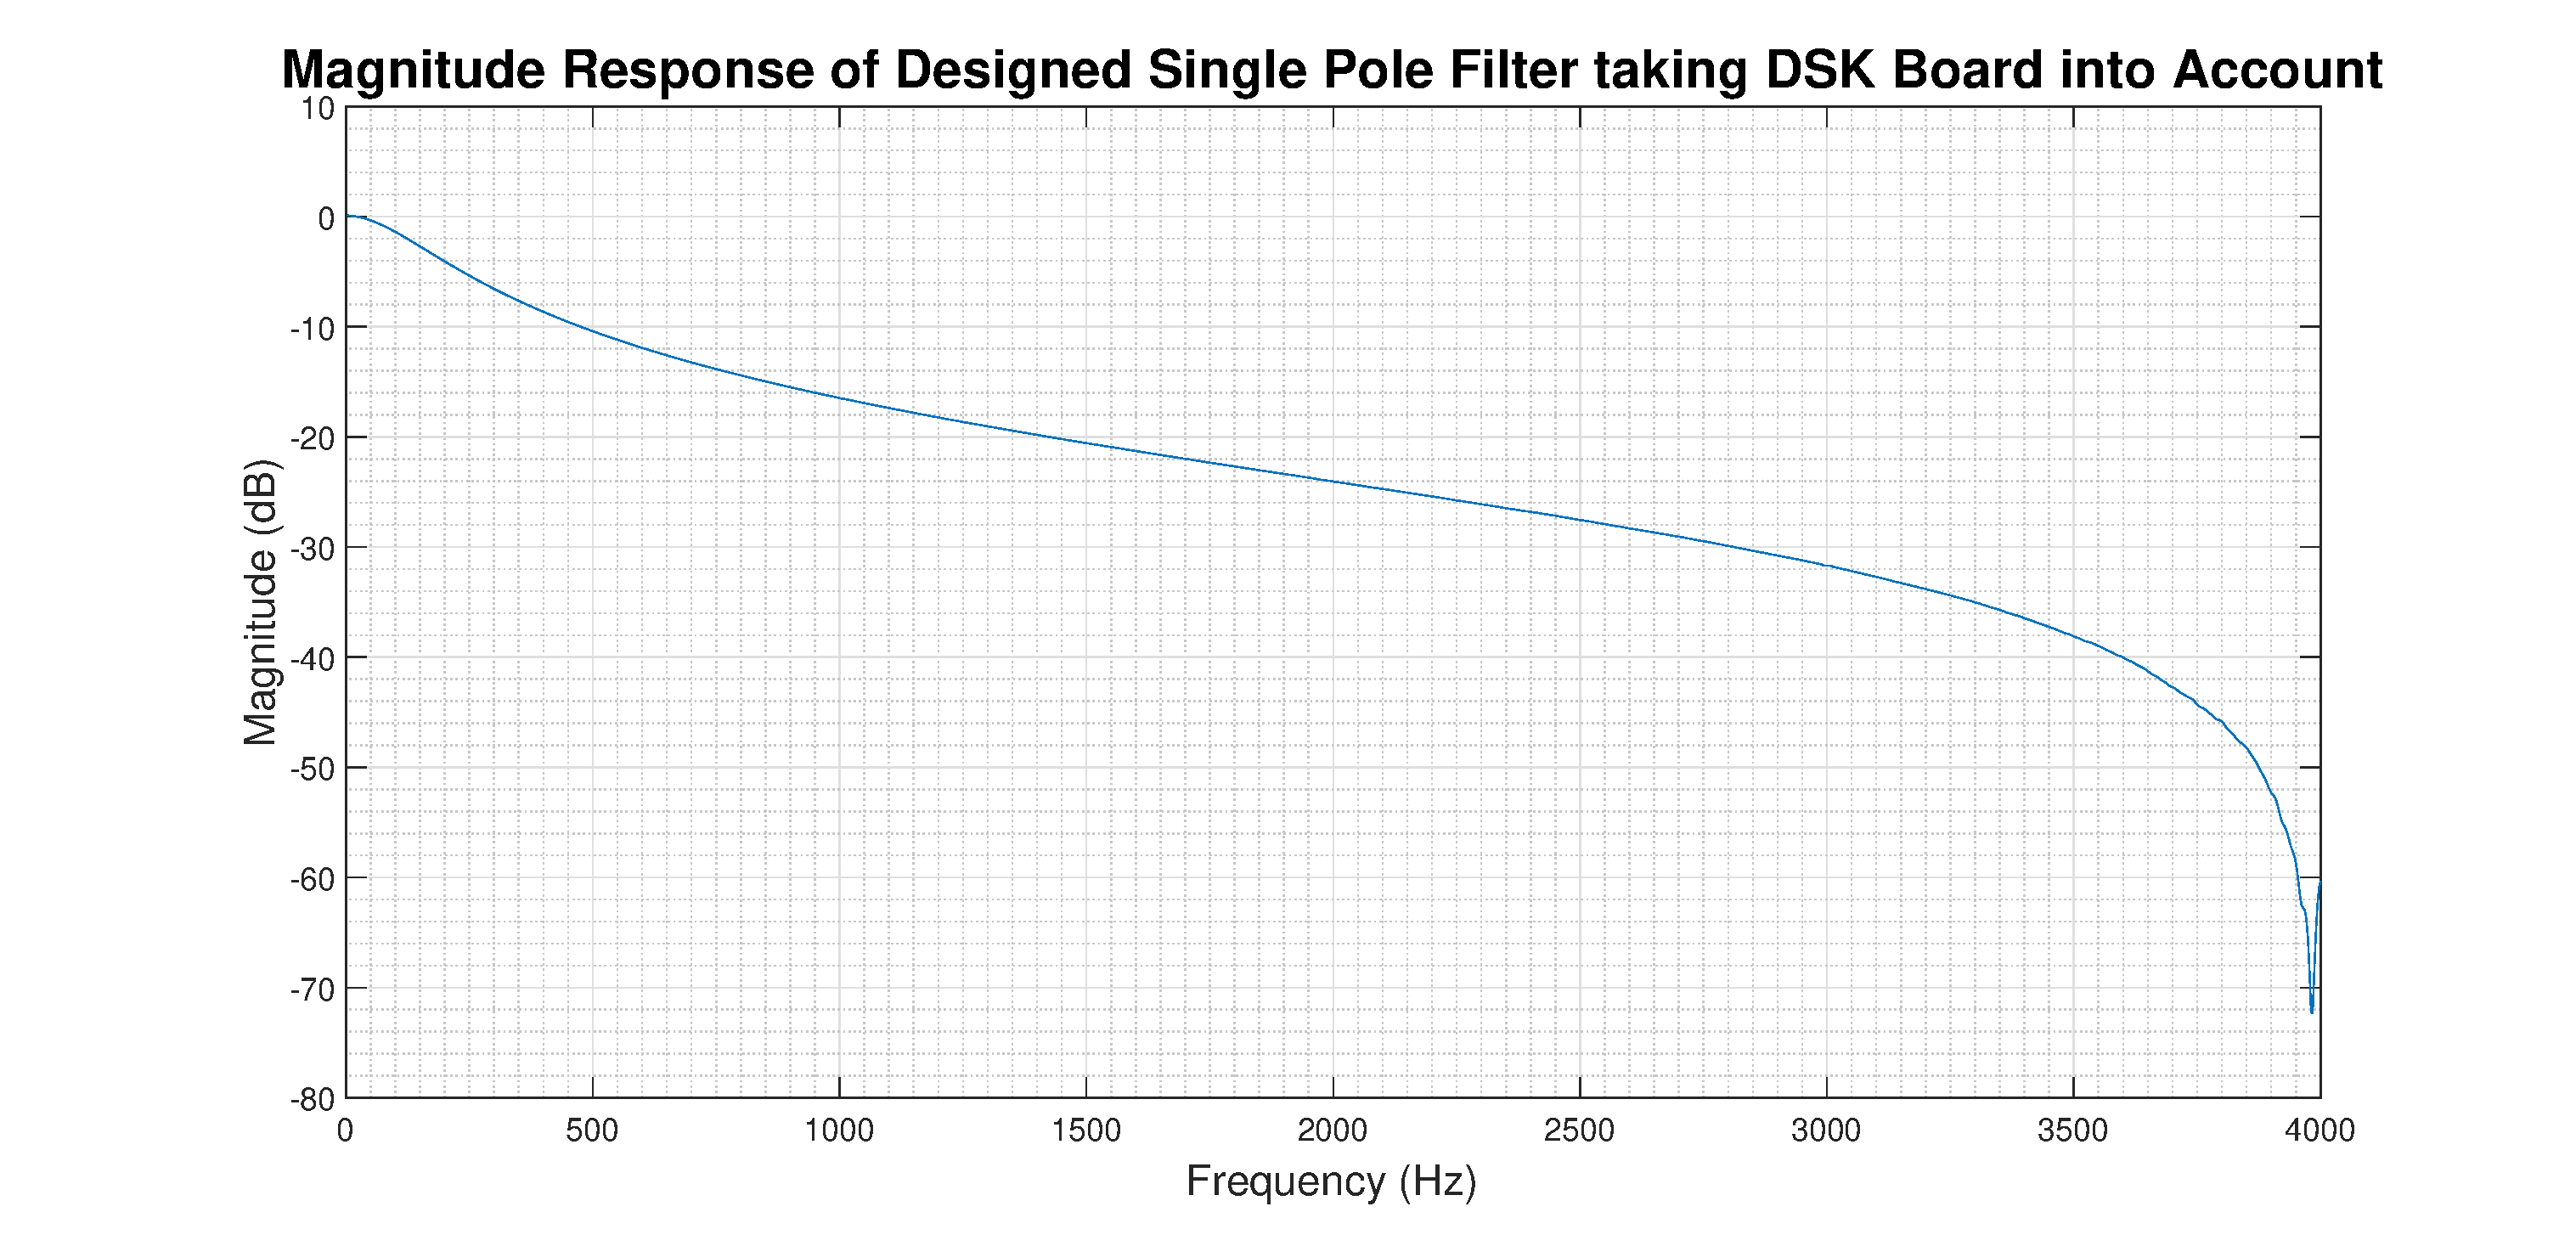
\includegraphics[width=0.49\textwidth]{mag_response_designed_single_pole_filter_with_DSK_taken_into_account}
    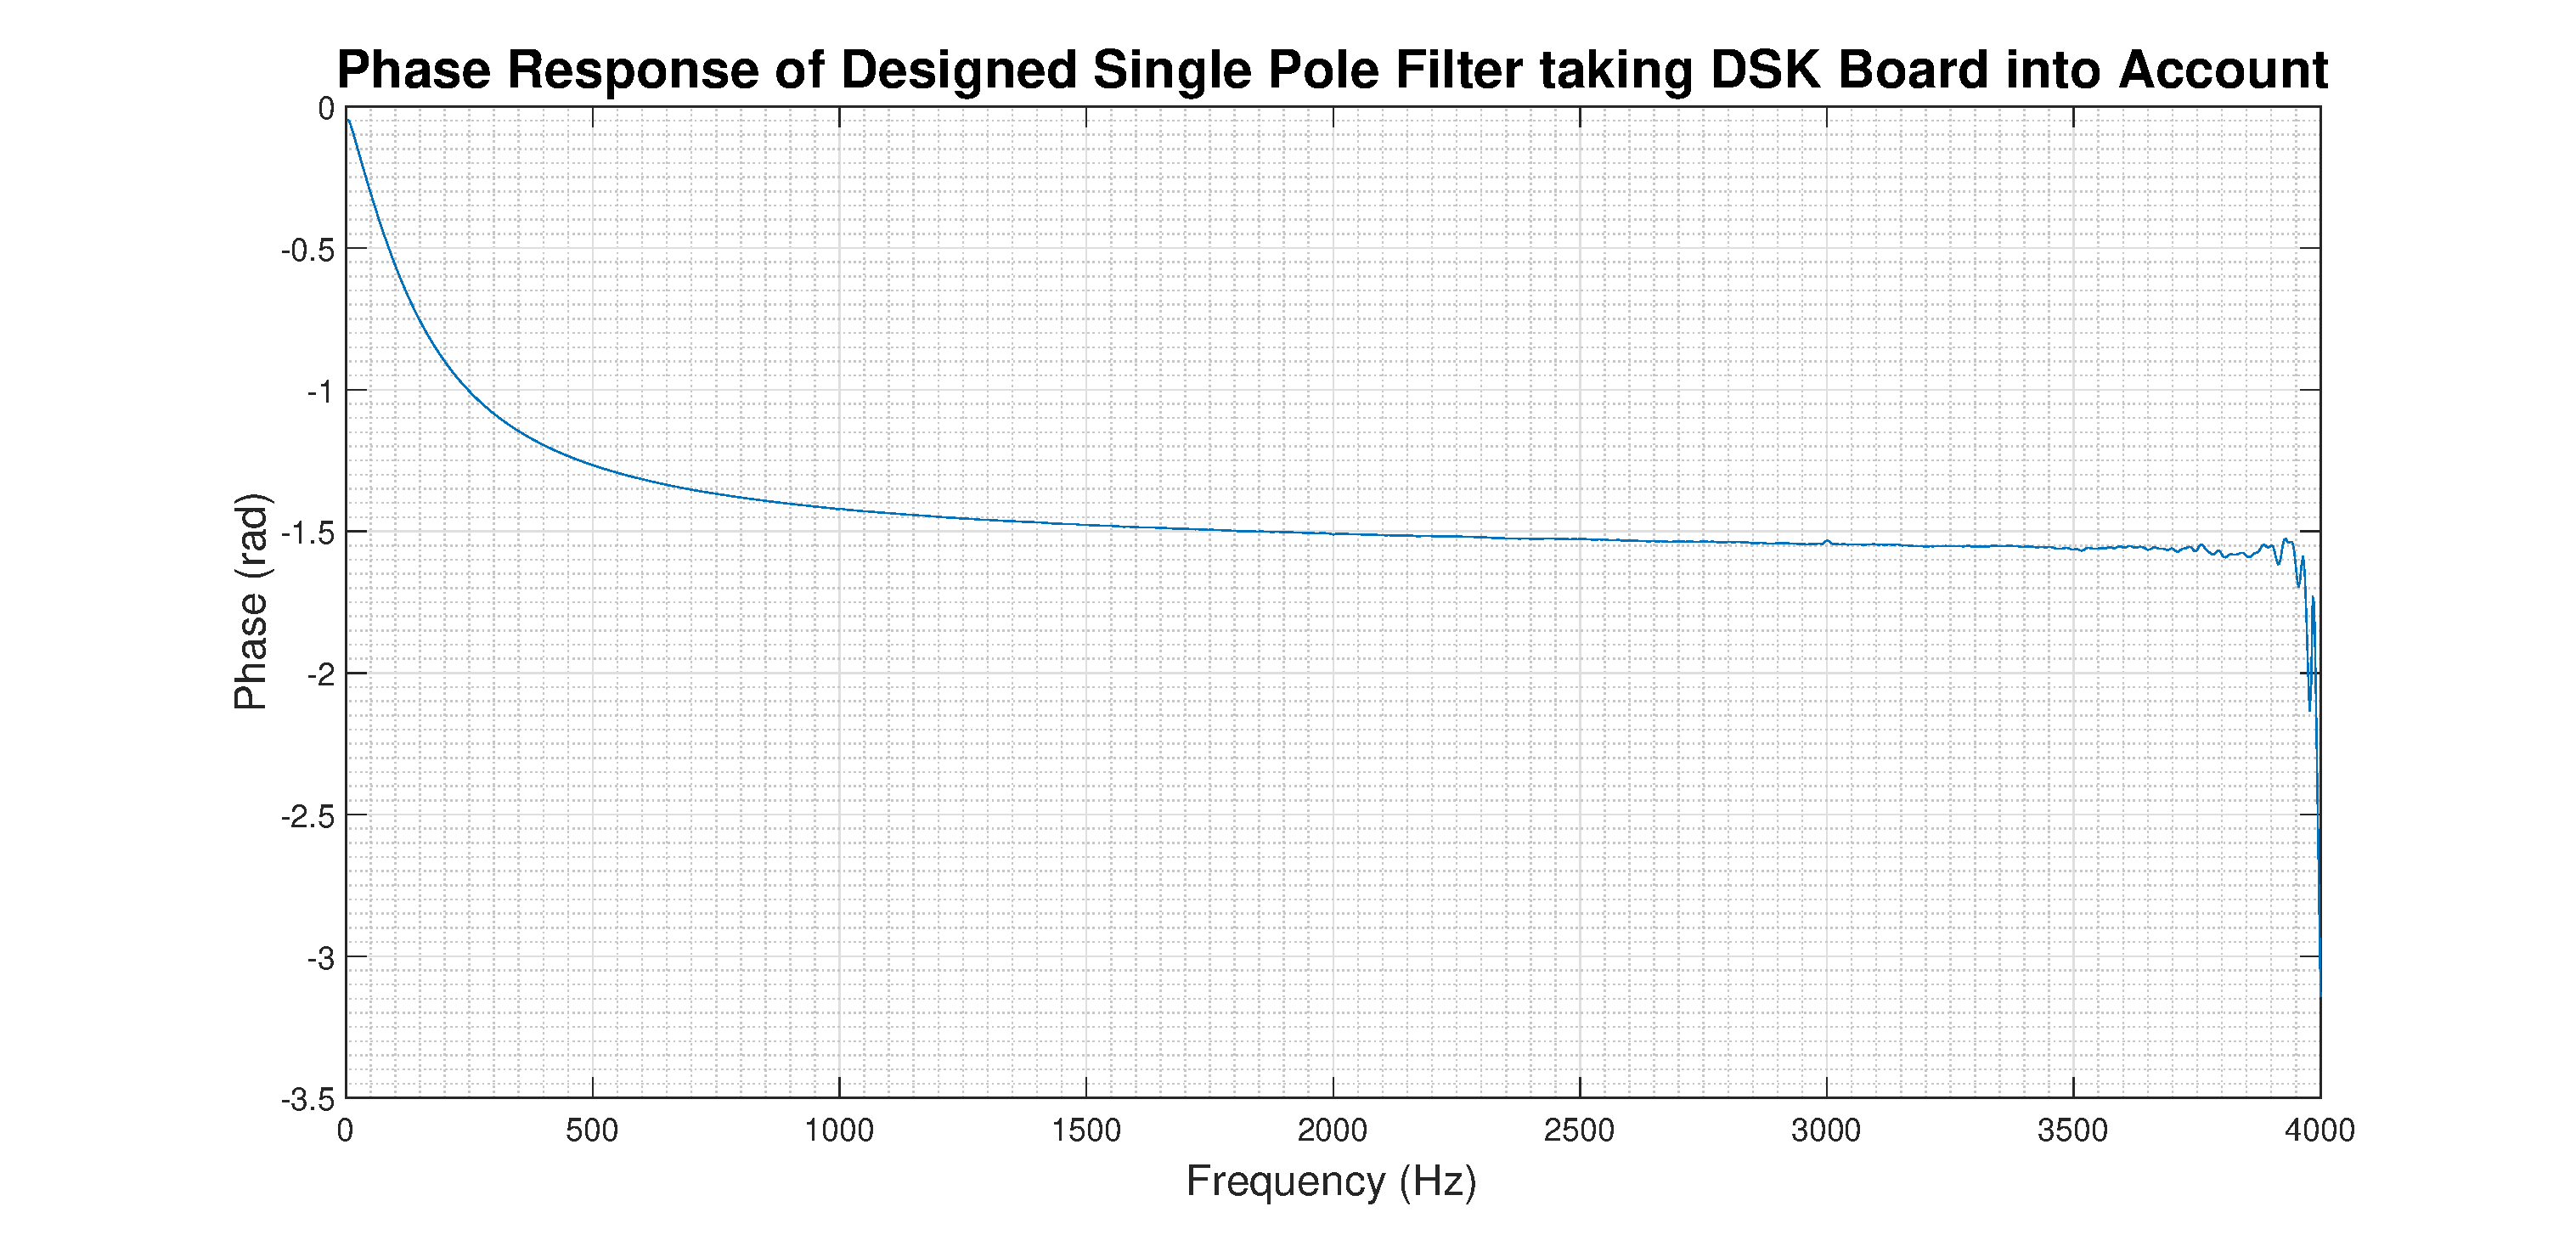
\includegraphics[width=0.49\textwidth]{monir_update}
    \caption{Frequency response of filter taking  $TMS320C6713 \ DSK$ board's inherent response into account}
    \label{fig:old_filter_subtracted}
\end{figure}

Figure \ref{fig:time_constat_actual} shows the actual corner frequency of the filter offset introduced by the $DSK$ board is taken into account. 

\begin{figure}[H]
    \centering
    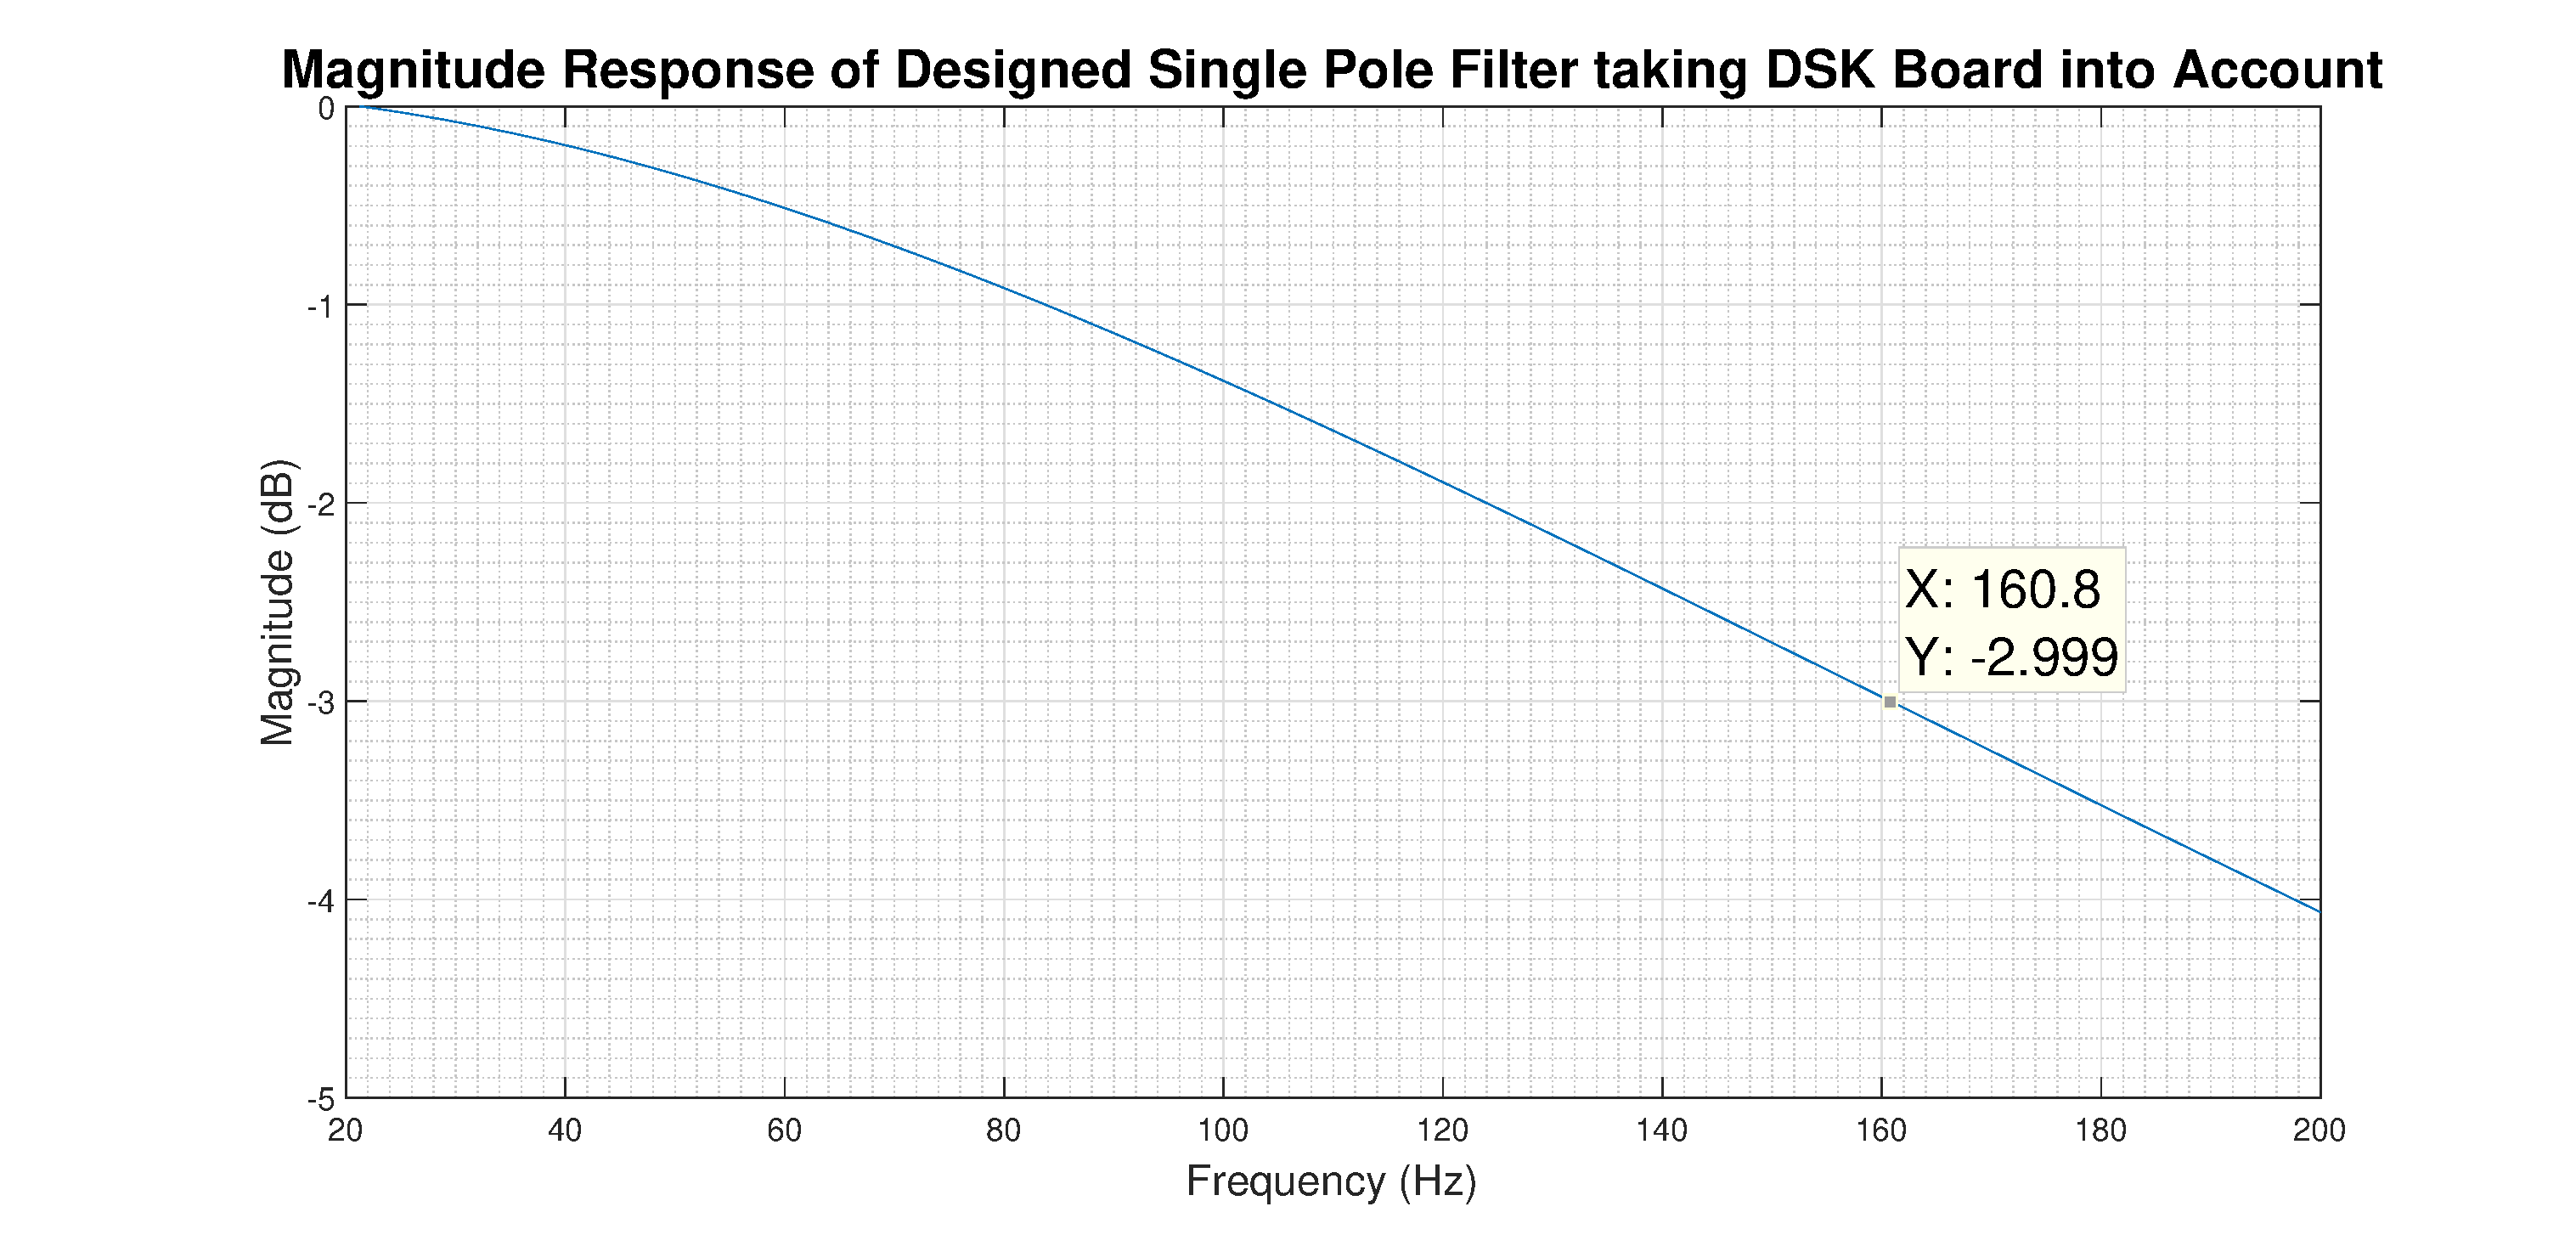
\includegraphics[width=0.8\textwidth]{time_constant_measured}
    \caption{Frequency response of filter taking  $TMS320C6713 \ DSK$ board's inherent response into account}
    \label{fig:time_constat_actual}
\end{figure}

\newpage
\textbf{In section \ref{sec:time_const}, the time constant of the digital filter was calculated to be $0.840ms$. This is slightly off from the theoretical value for the digital filter which is $1.001ms$. The difference can be attributed to the inherent frequency response of the DSK board. Using $f_{c} = 160.8Hz$, the time constant of the filter comes to $0.990ms$. This is significantly closer to the theoretical value of $1.00ms$ and confirms that the digital filter designed in section \ref{sec:design_of_digital_filter} has been implemented correctly on the $DSK$ board. Table \ref{tab:time_constants} summarises the data obtained.}

\begin{table}[H]
\centering
\begin{tabular}{lcccc}
\cline{2-5}
\multicolumn{1}{l|}{} & \multicolumn{1}{c|}{\begin{tabular}[c]{@{}c@{}}Analogue\\   Filter\end{tabular}} & \multicolumn{1}{c|}{\begin{tabular}[c]{@{}c@{}}Ideal Digital \\ Filter\end{tabular}} & \multicolumn{1}{c|}{\begin{tabular}[c]{@{}c@{}}Digital Filter without taking\\   DSK offset into Account\end{tabular}} & \multicolumn{1}{c|}{\begin{tabular}[c]{@{}c@{}}Digital Filter taking DSK \\ offset into account\end{tabular}} \\ \hline
\multicolumn{1}{|l|}{\begin{tabular}[c]{@{}l@{}}Corner\\   Frequency / Hz\end{tabular}} & \multicolumn{1}{c|}{159.15} & \multicolumn{1}{c|}{158.94} & \multicolumn{1}{c|}{189.47} & \multicolumn{1}{c|}{160.80} \\ \hline
\multicolumn{1}{|l|}{\begin{tabular}[c]{@{}l@{}}Time\\   Constant / ms\end{tabular}} & \multicolumn{1}{c|}{1.000} & \multicolumn{1}{c|}{1.001} & \multicolumn{1}{c|}{0.840} & \multicolumn{1}{c|}{0.990} \\ \hline
 & \multicolumn{1}{l}{} & \multicolumn{1}{l}{} & \multicolumn{1}{l}{} & \multicolumn{1}{l}{}
\end{tabular}
\caption{Corner frequencies and time constants overview}
\label{tab:time_constants}
\end{table}


Lastly, figure \ref{fig:RC_comparison} shows how the frequency response of the digital filter compares to that of the analogue RC filter. The graph shows that the bilinear transfomation has been very effectively in mapping the analogue filter to the digital domain. \textbf{Near $4kHz$, both magnitude and phase response diverge slightly from the ideal response due to the anti-aliasing filter.} 

\begin{figure}[H]
    \centering
    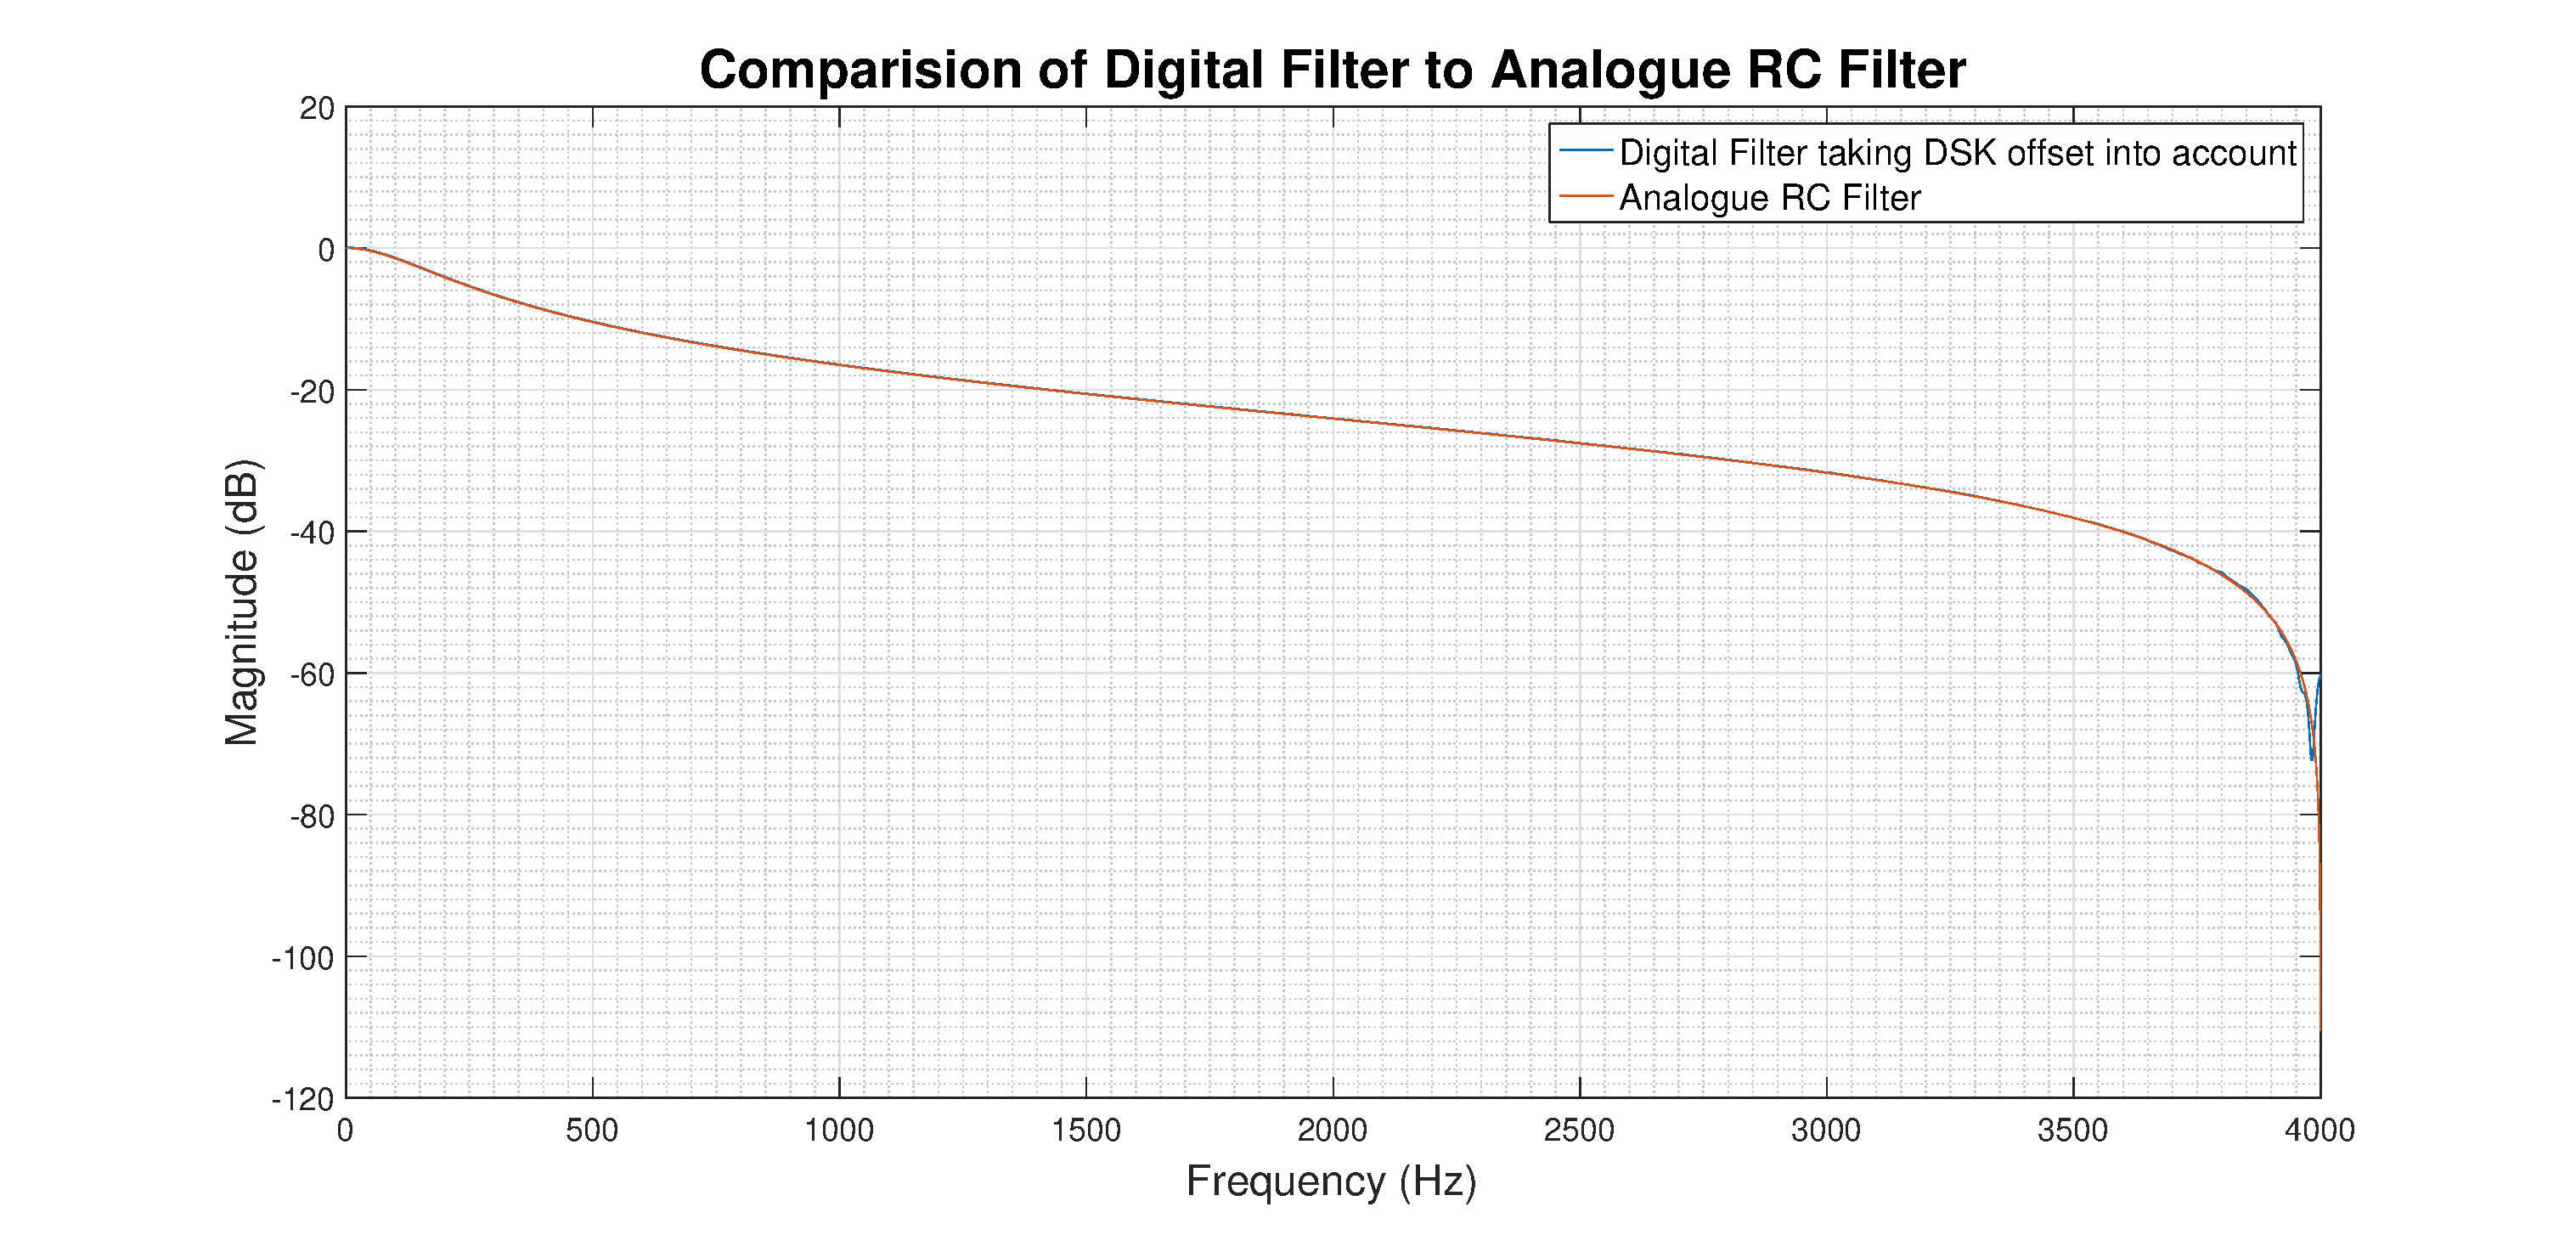
\includegraphics[width=0.80\textwidth]{mag_response_comparison}
    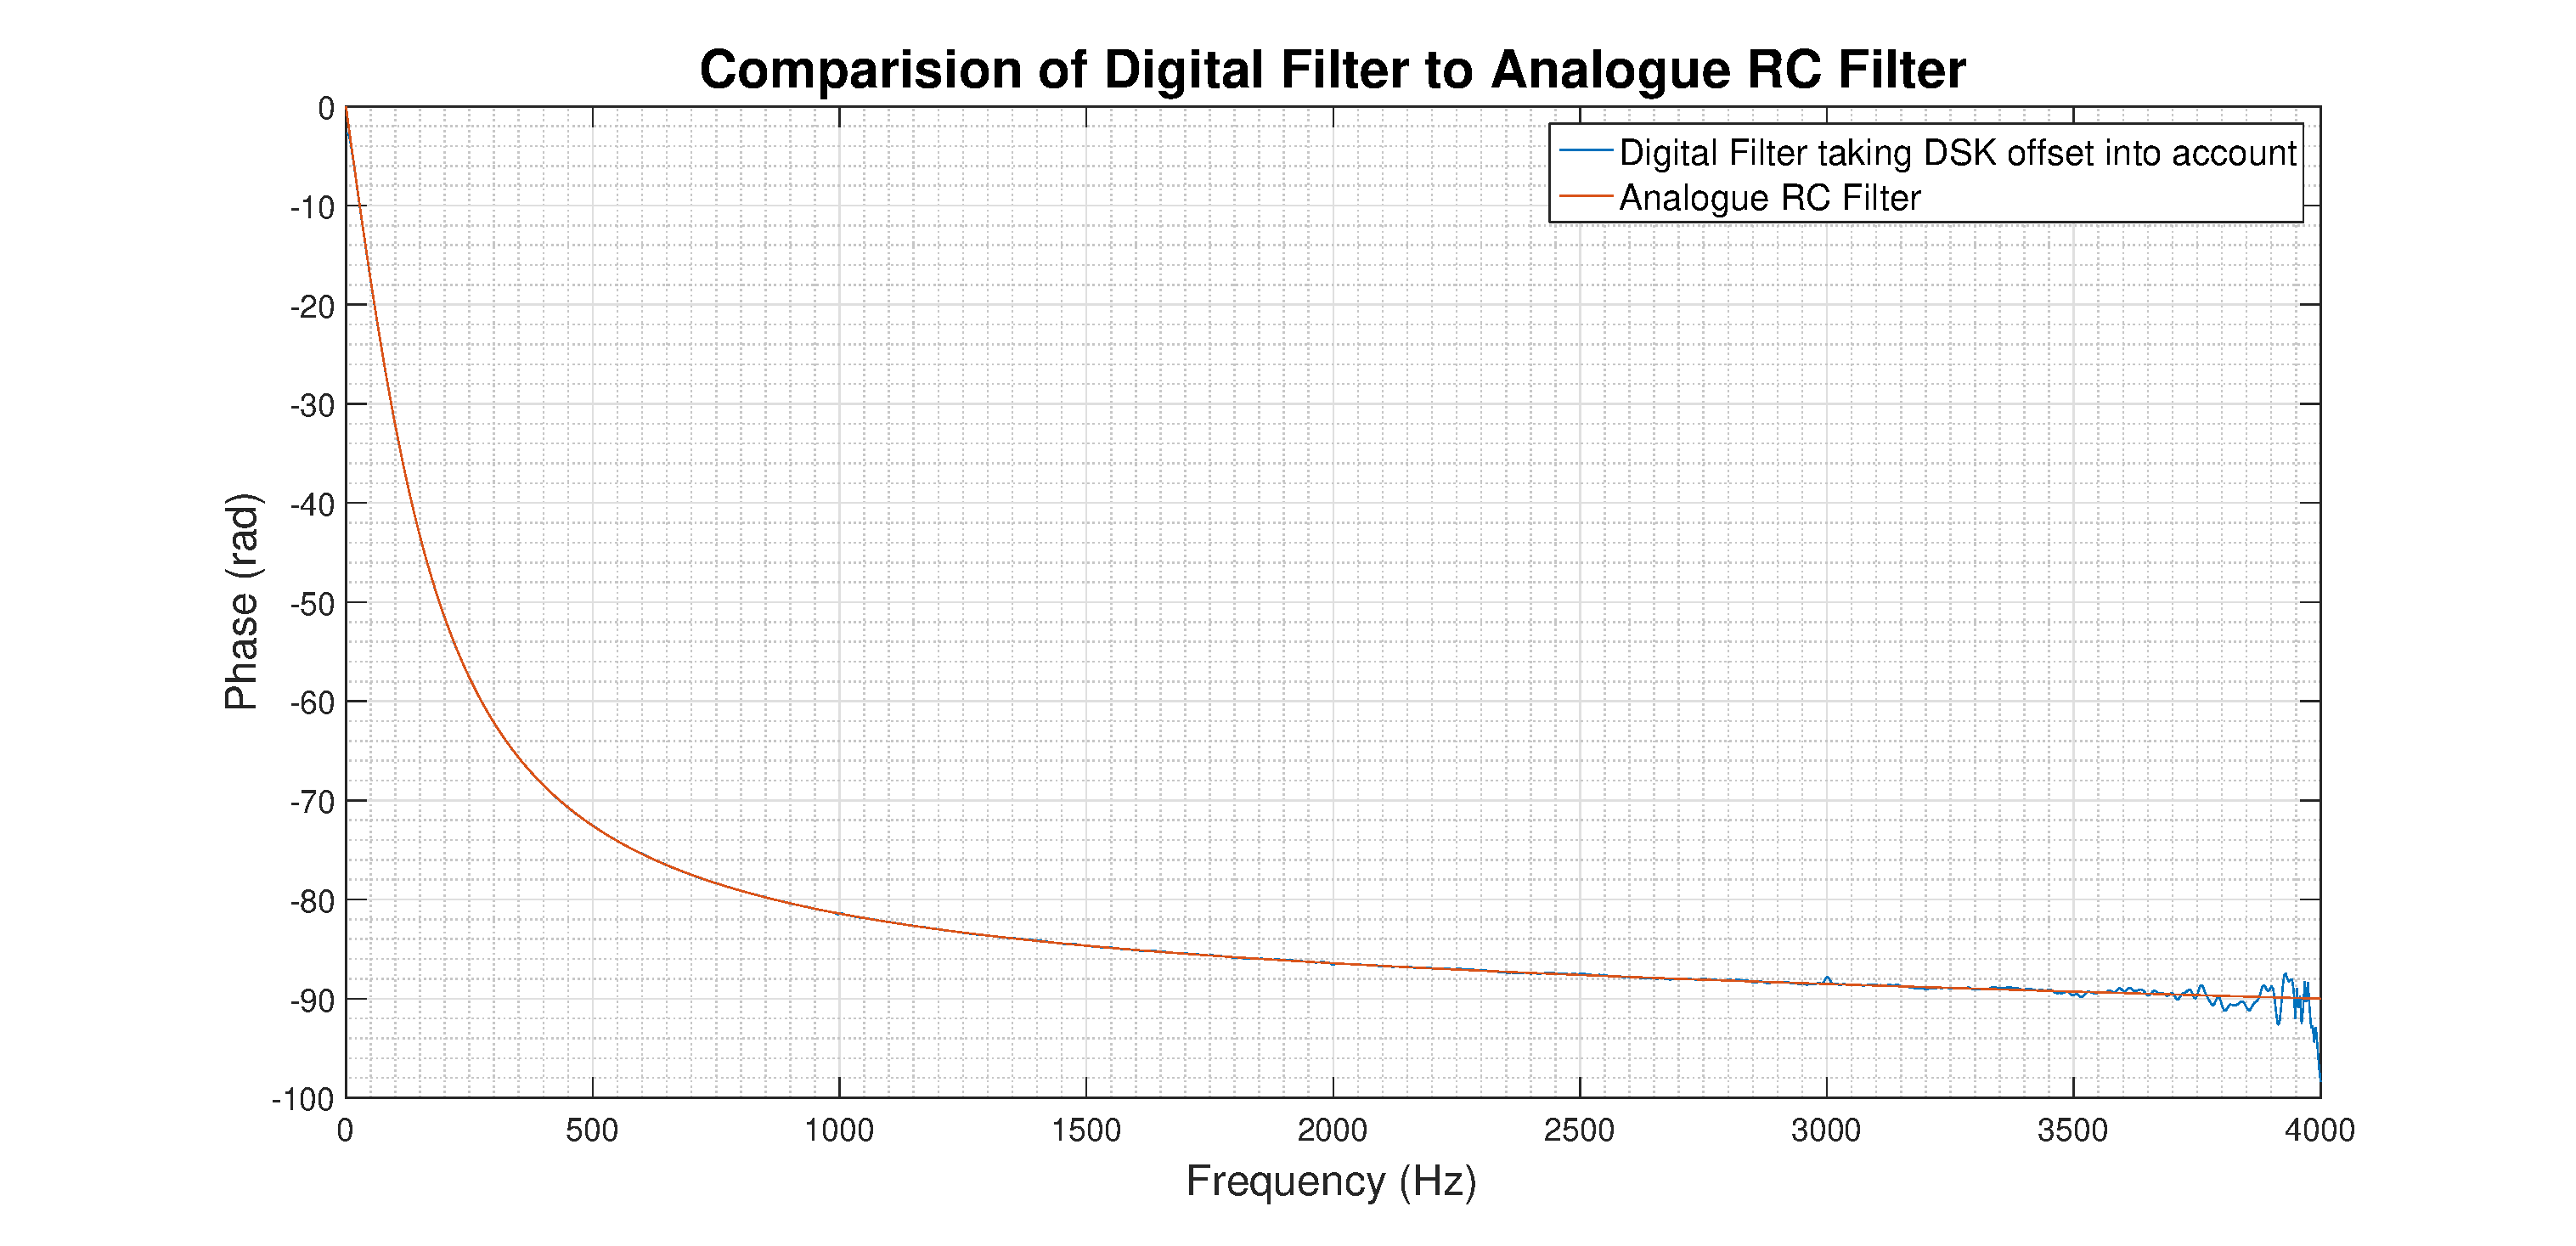
\includegraphics[width=0.80\textwidth]{phase_response_comparison}
    \caption{Comparision of frequency response of the digital filter and the analogue filter}
    \label{fig:RC_comparison}
\end{figure}

\newpage
\section{Bandpass Filter}\label{sec:bandpass_design}
In laboratory 5, an elliptical filter has to be designed. The specifications for the filter are:
\begin{itemize}
    \item Order: 4th
    \item Passband: $180Hz \ - \ 450Hz$
    \item Passband ripple: $0.4dB$
    \item Stopband attenuation: $23dB$ 
\end{itemize}

The filter is designed using the MATLAB code presented in lisiting \ref{lst:MATLAB_elliptical}.

\begin{listing}[H]
\begin{minted}[fontsize=\scriptsize,linenos]{MATLAB}
fsamp = 8000;                   % defines the sampling frequency
order = 4;                      % defines the order of the digital filter
passband_ripple = 0.4;          % defines the passband ripple
stopband_attenuation = 23;      % defines the stopband attenuation of the filter
Wp = [180 450]/(0.5*fsamp);     % normalising edge frequencies of passband


% ellip function designs filter of order 2n
[b, a] = ellip(order/2, passband_ripple, stopband_ripple, Wp, "bandpass");
\end{minted}
\caption{MATLAB code to generate coefficients for an elliptical filter} 
\label{lst:MATLAB_elliptical}
\end{listing}

The generated filter's response is shown in figure \ref{fig:elliptical_theoretical_response}. 

\begin{figure}[H]
    \centering
    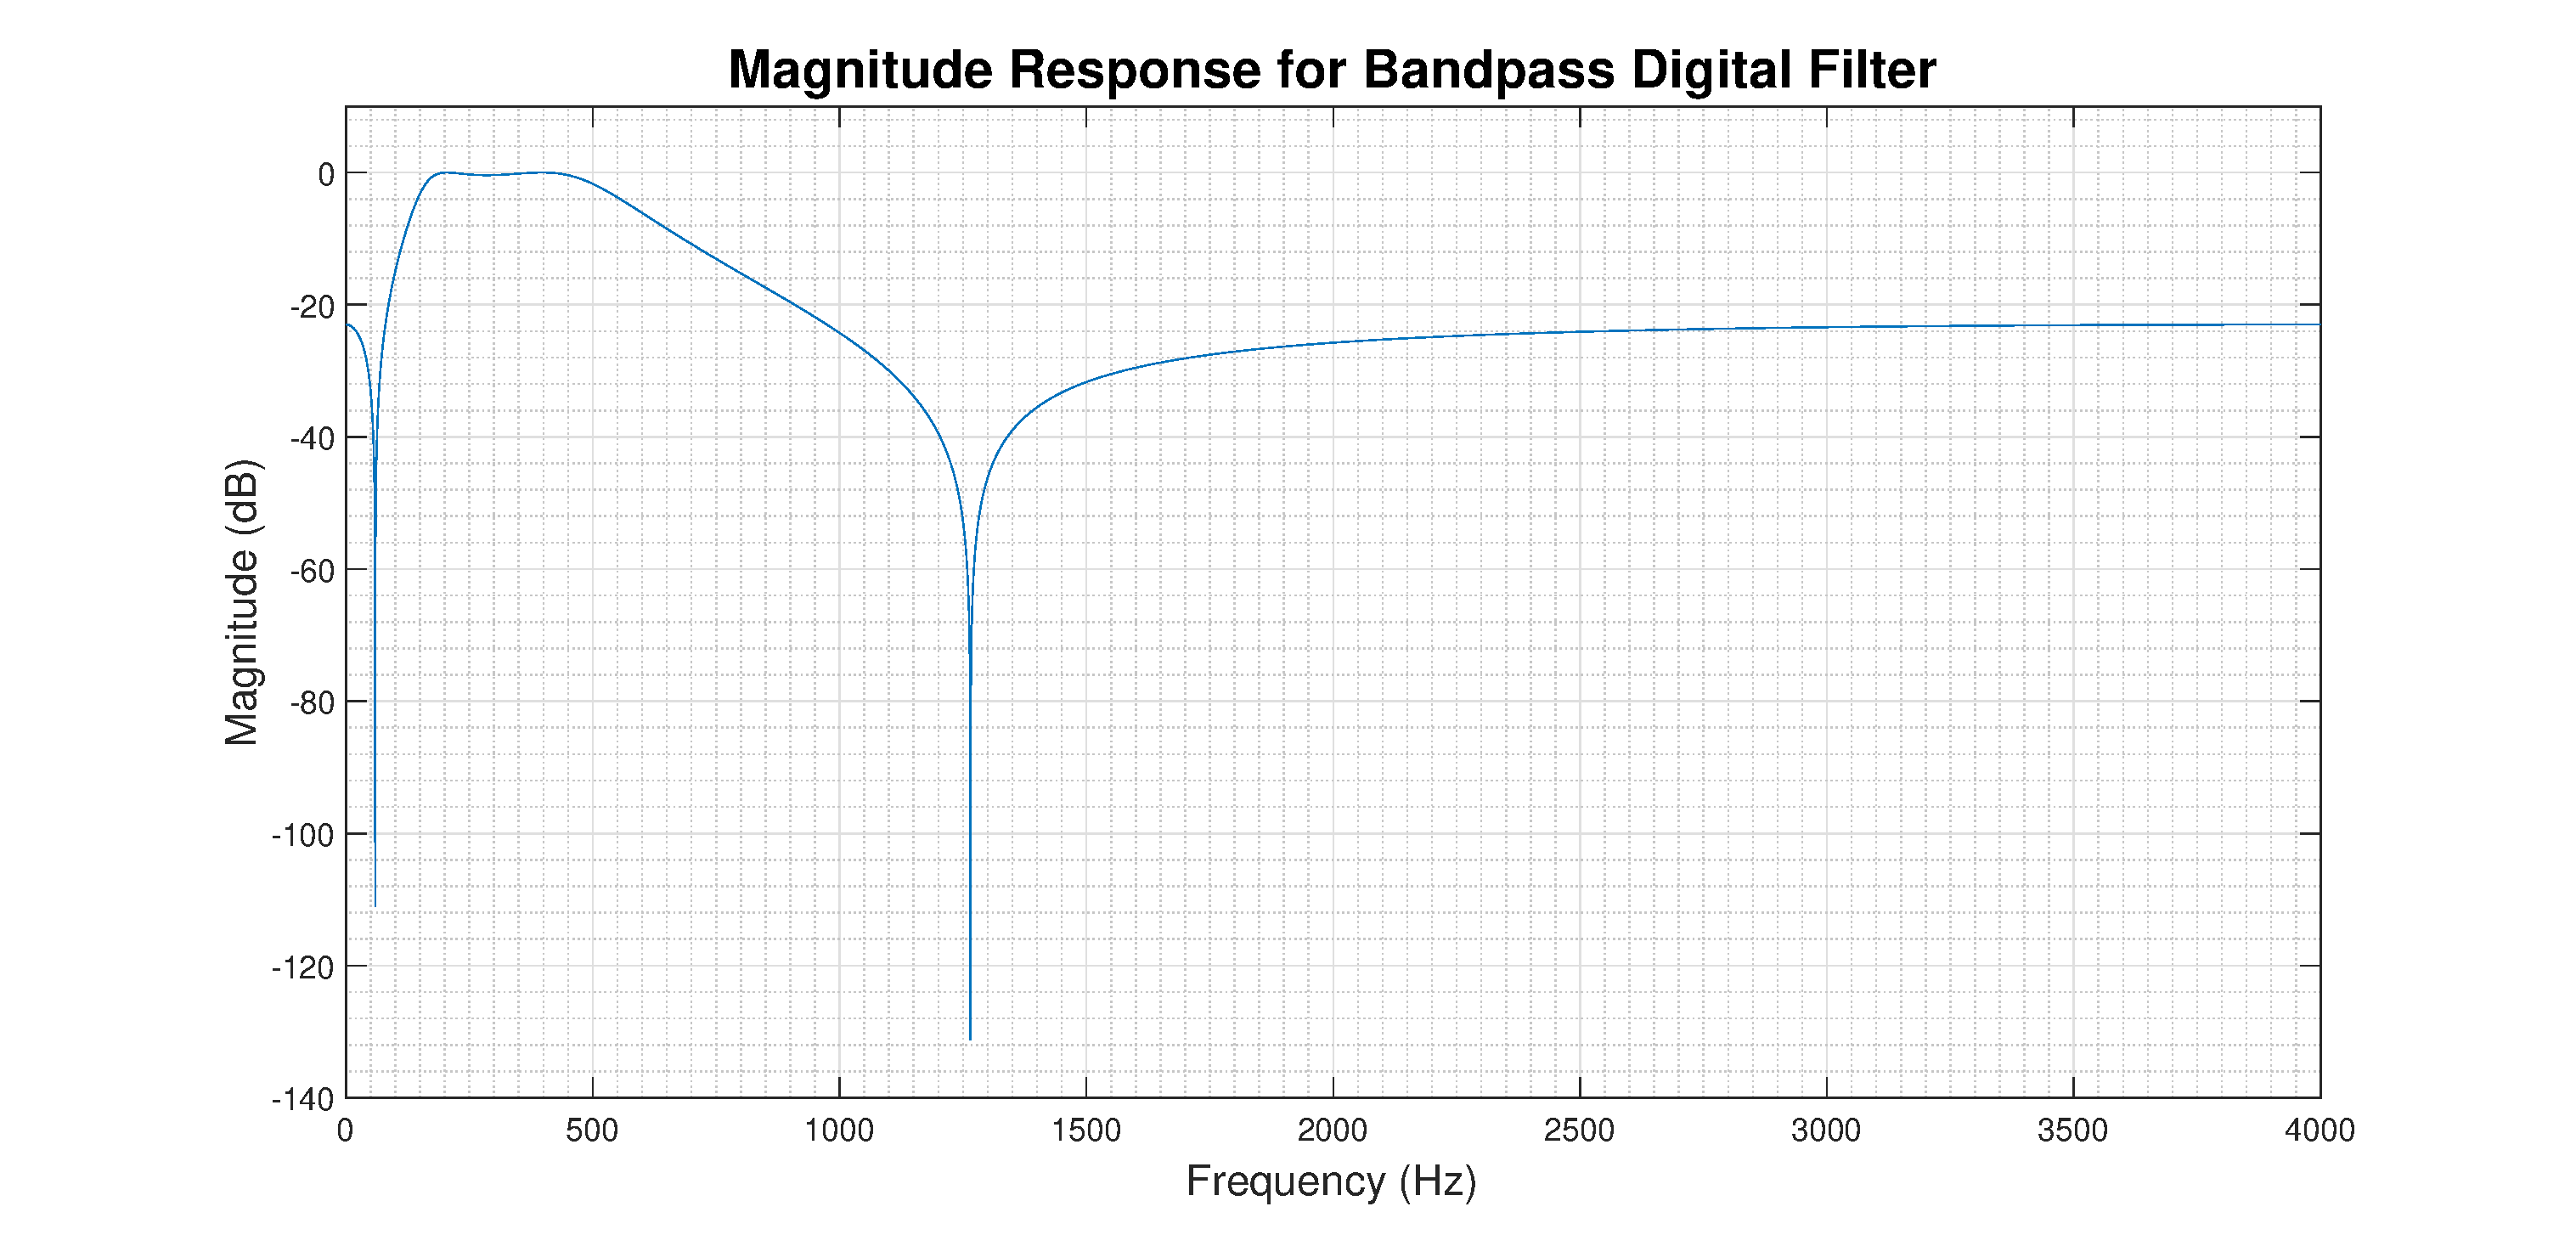
\includegraphics[width = 0.49\textwidth]{mag_response_digital_filter}
    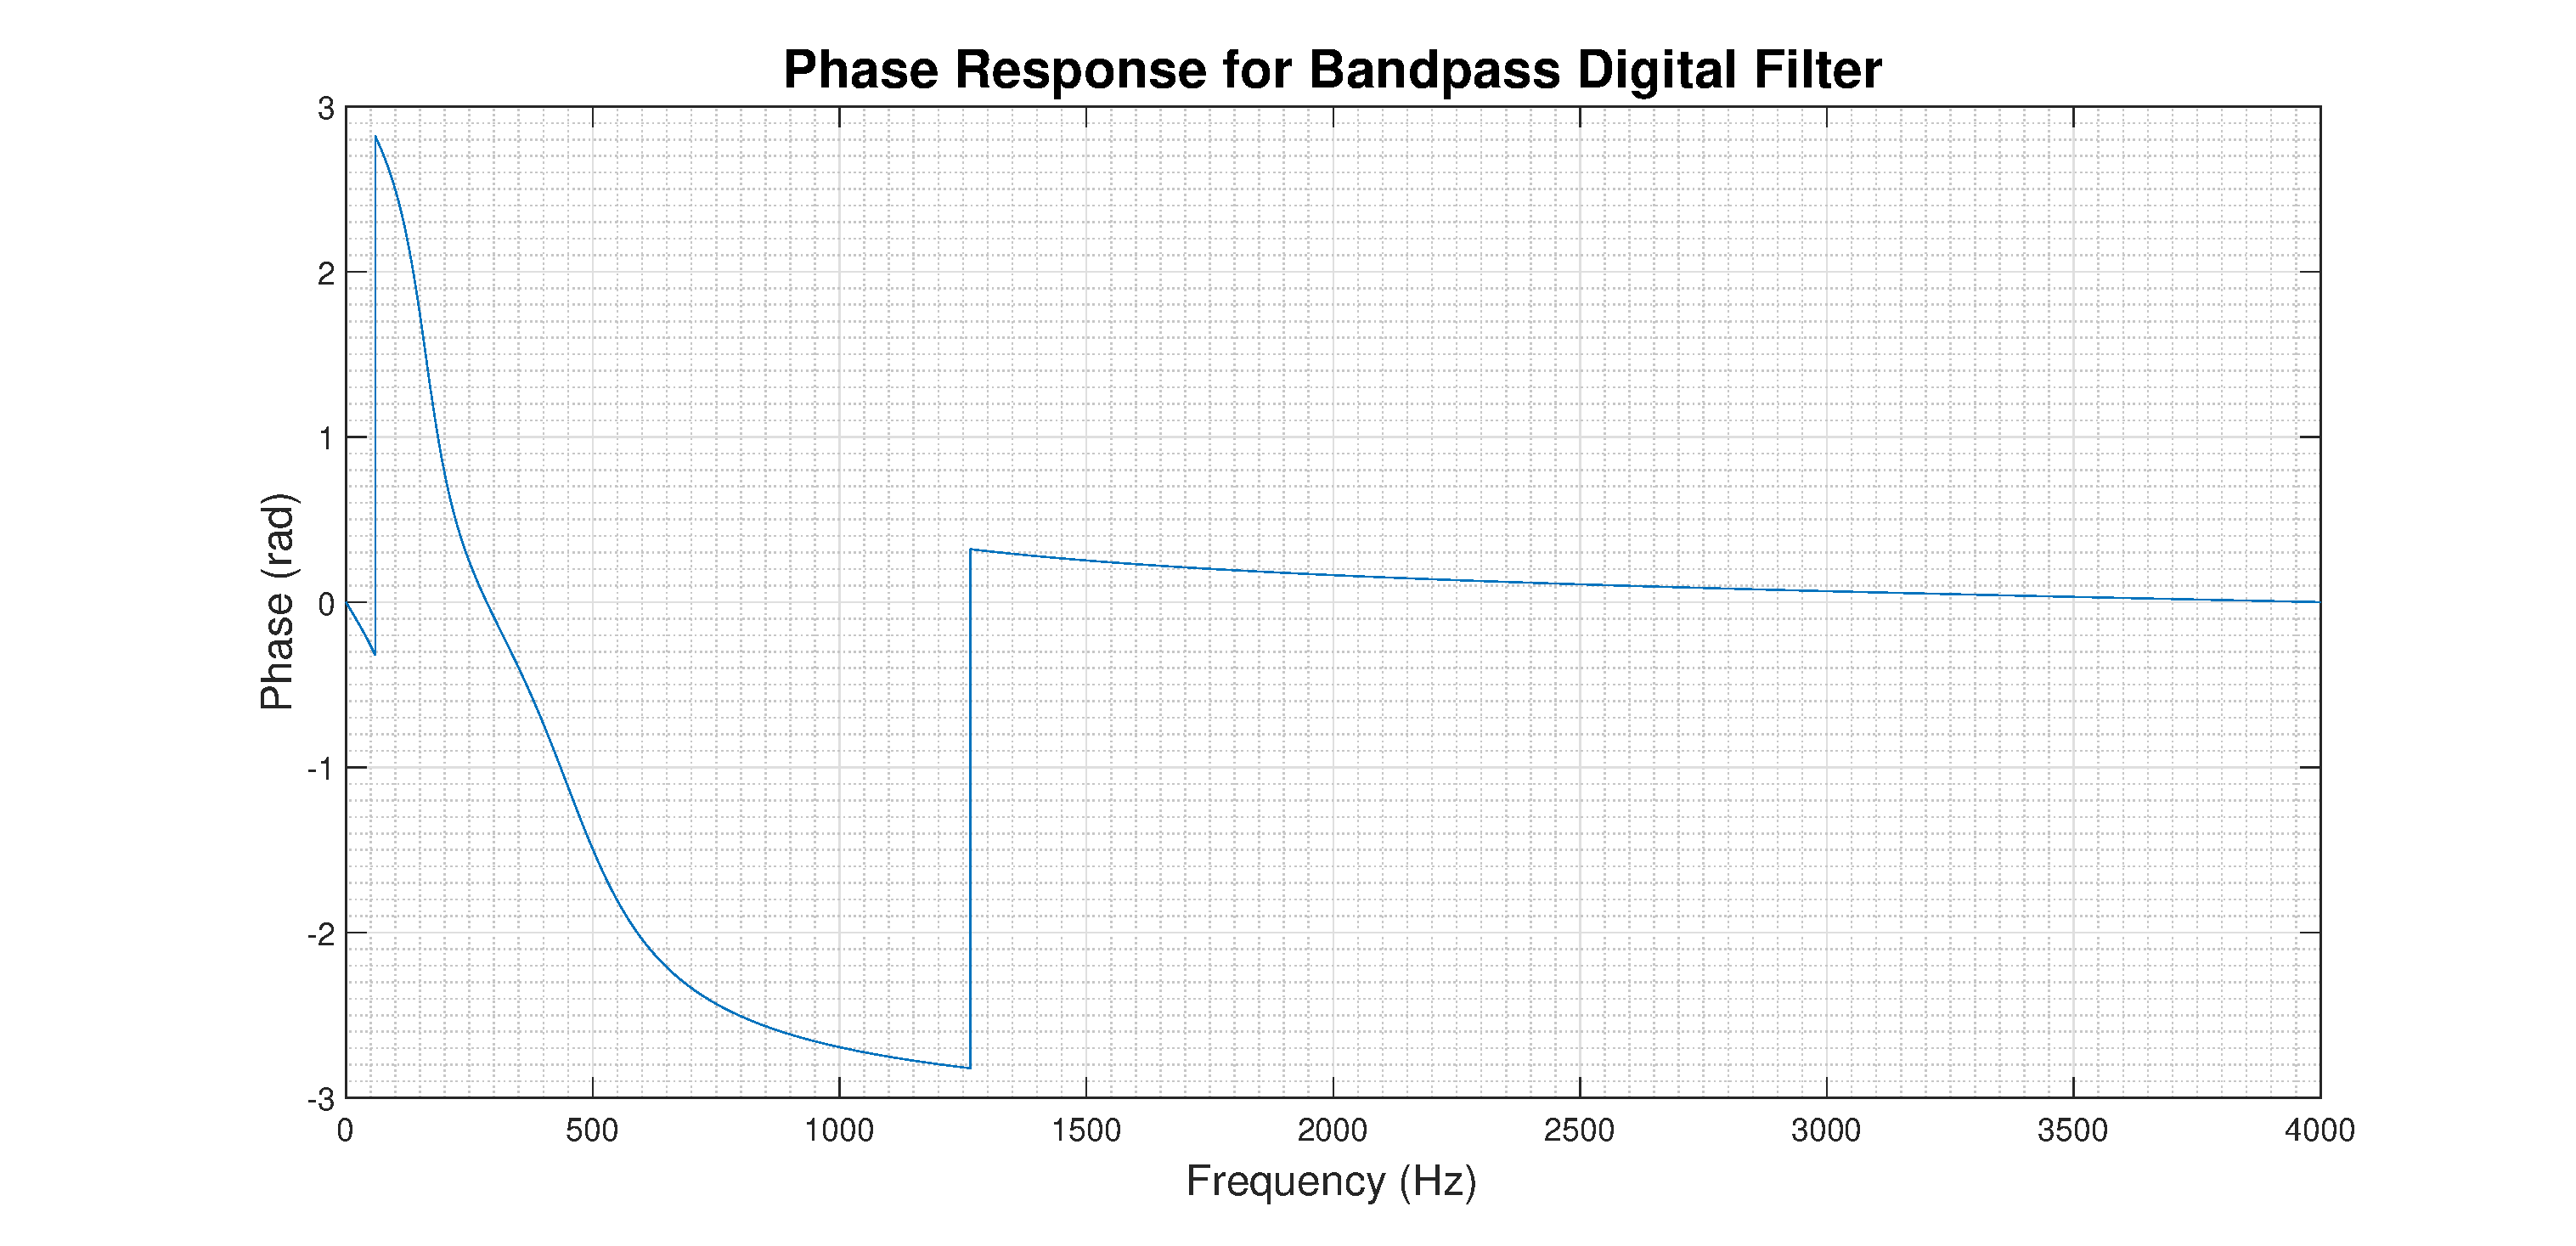
\includegraphics[width = 0.49\textwidth]{phase_response_digital_filter}
    \caption{Theoretical frequency response of digital filter}
    \label{fig:elliptical_theoretical_response}
\end{figure}

The first thing to notice is that the filter does not have a linear phase in the pass band. \textbf{A linear phase response is characteristic of FIR filters and a non-linear phase response is expected.} Secondly, the filter's magnitude response meets all the specifications set out in the laboratory script. Figure \ref{fig:passband_zoom} shows the magnitude response at specific frequencies.


\begin{figure}[H]
    \centering
    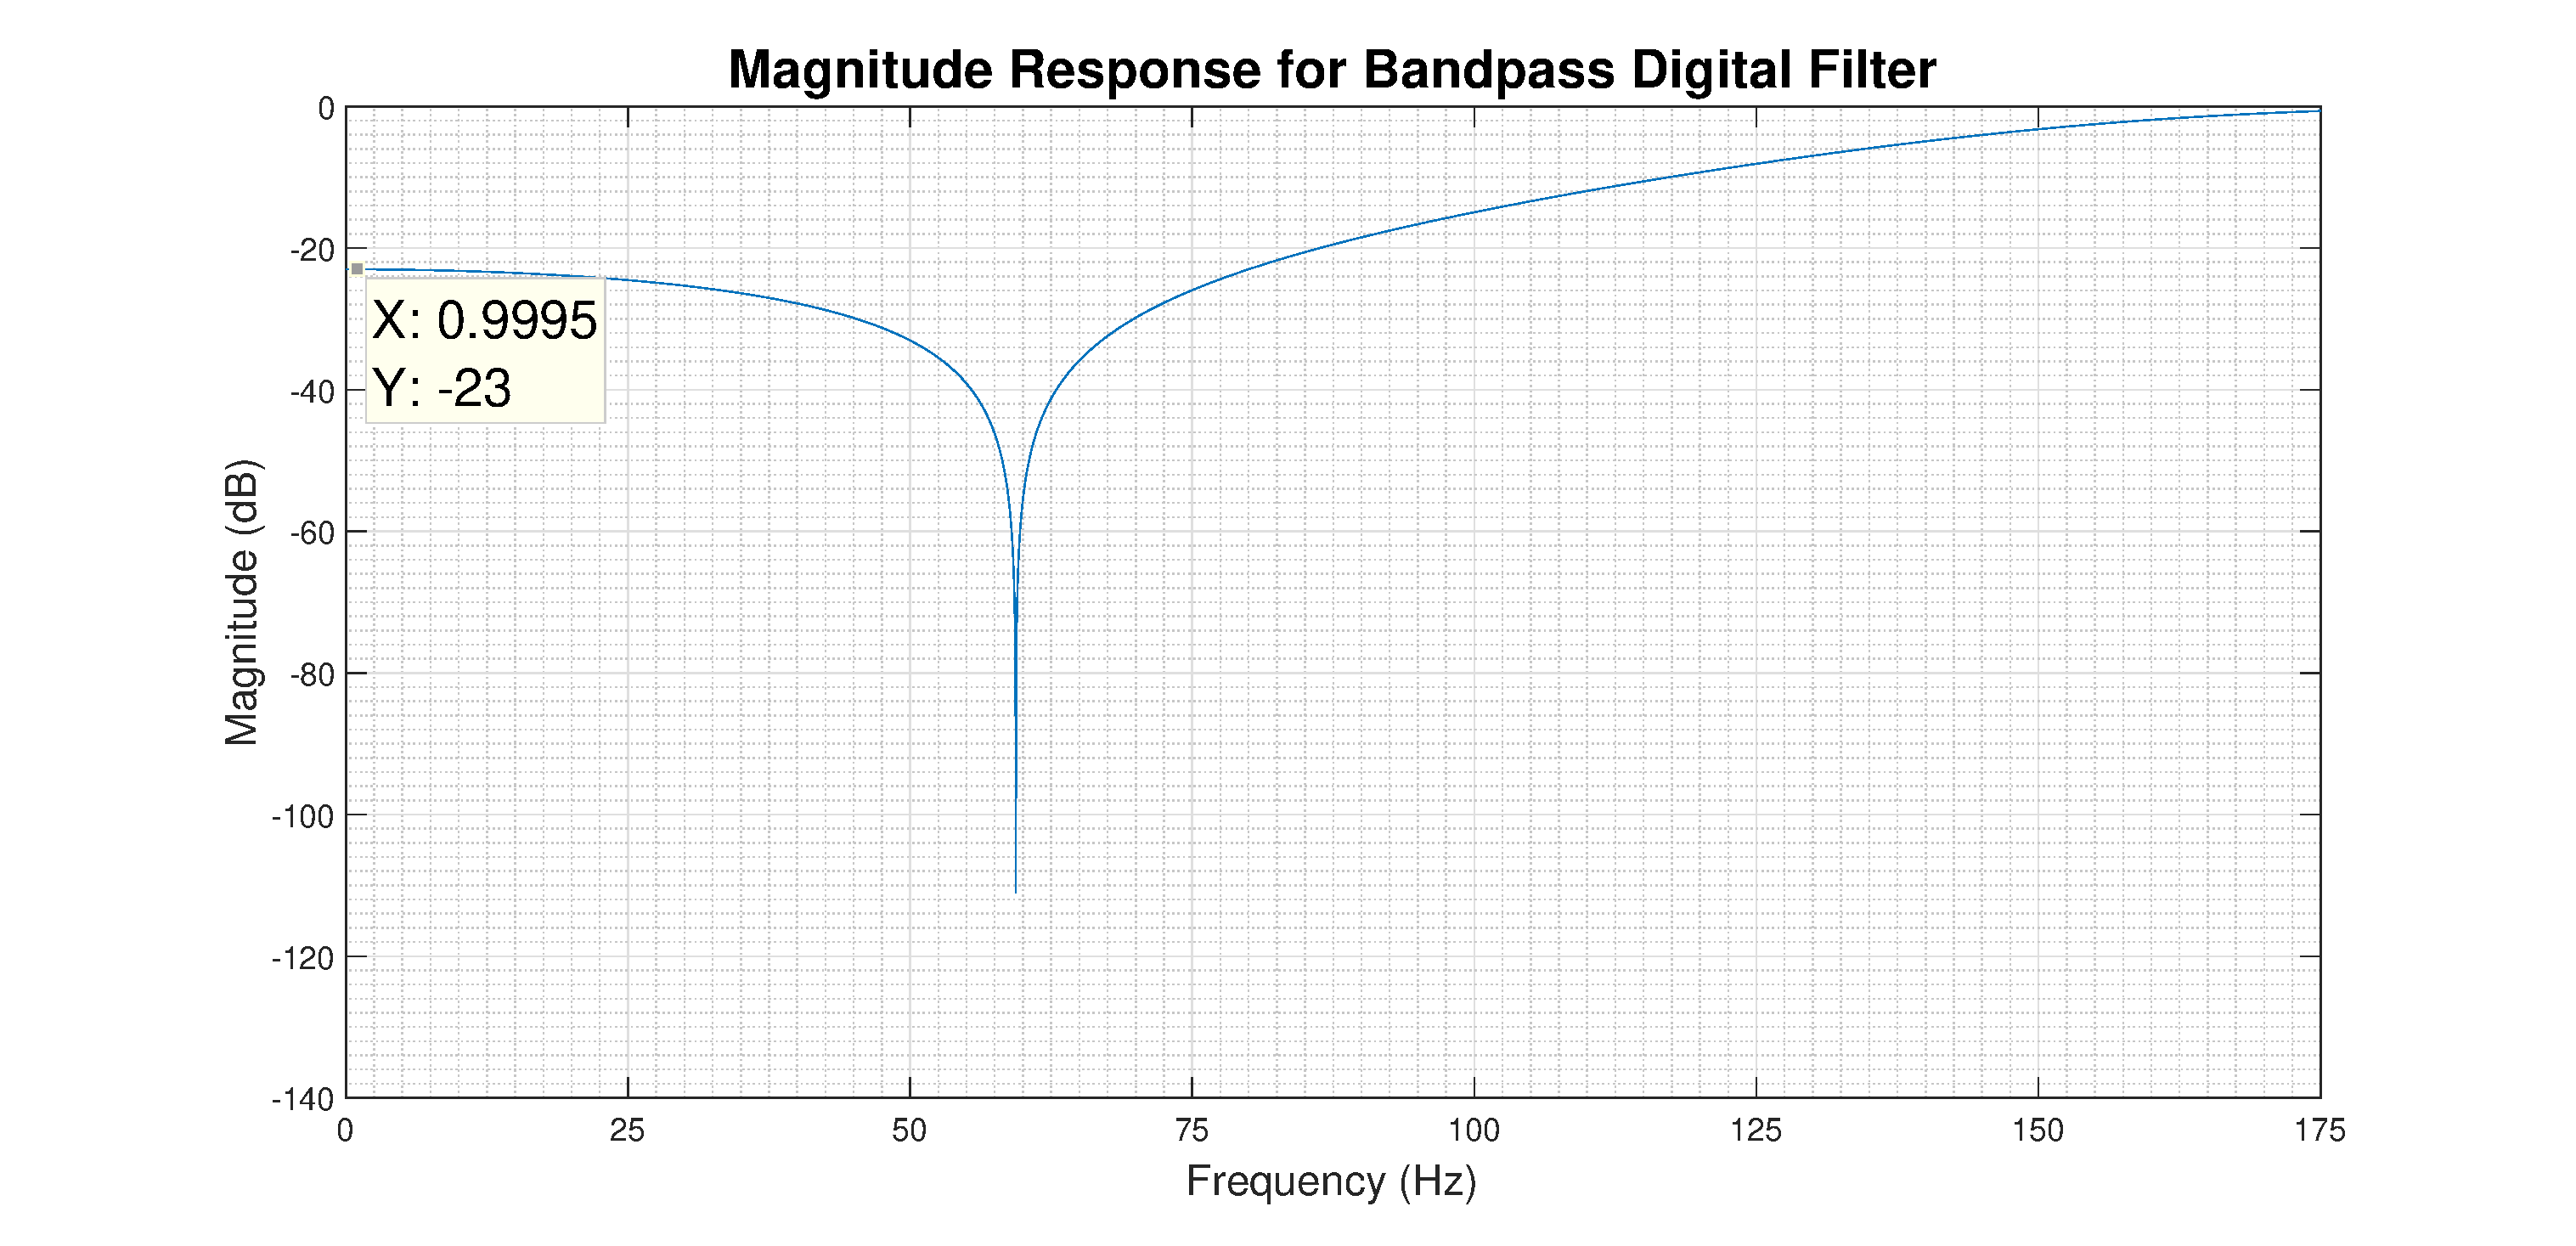
\includegraphics[width = 0.32\textwidth]{mag_response_digital_filter_stopband_left}
    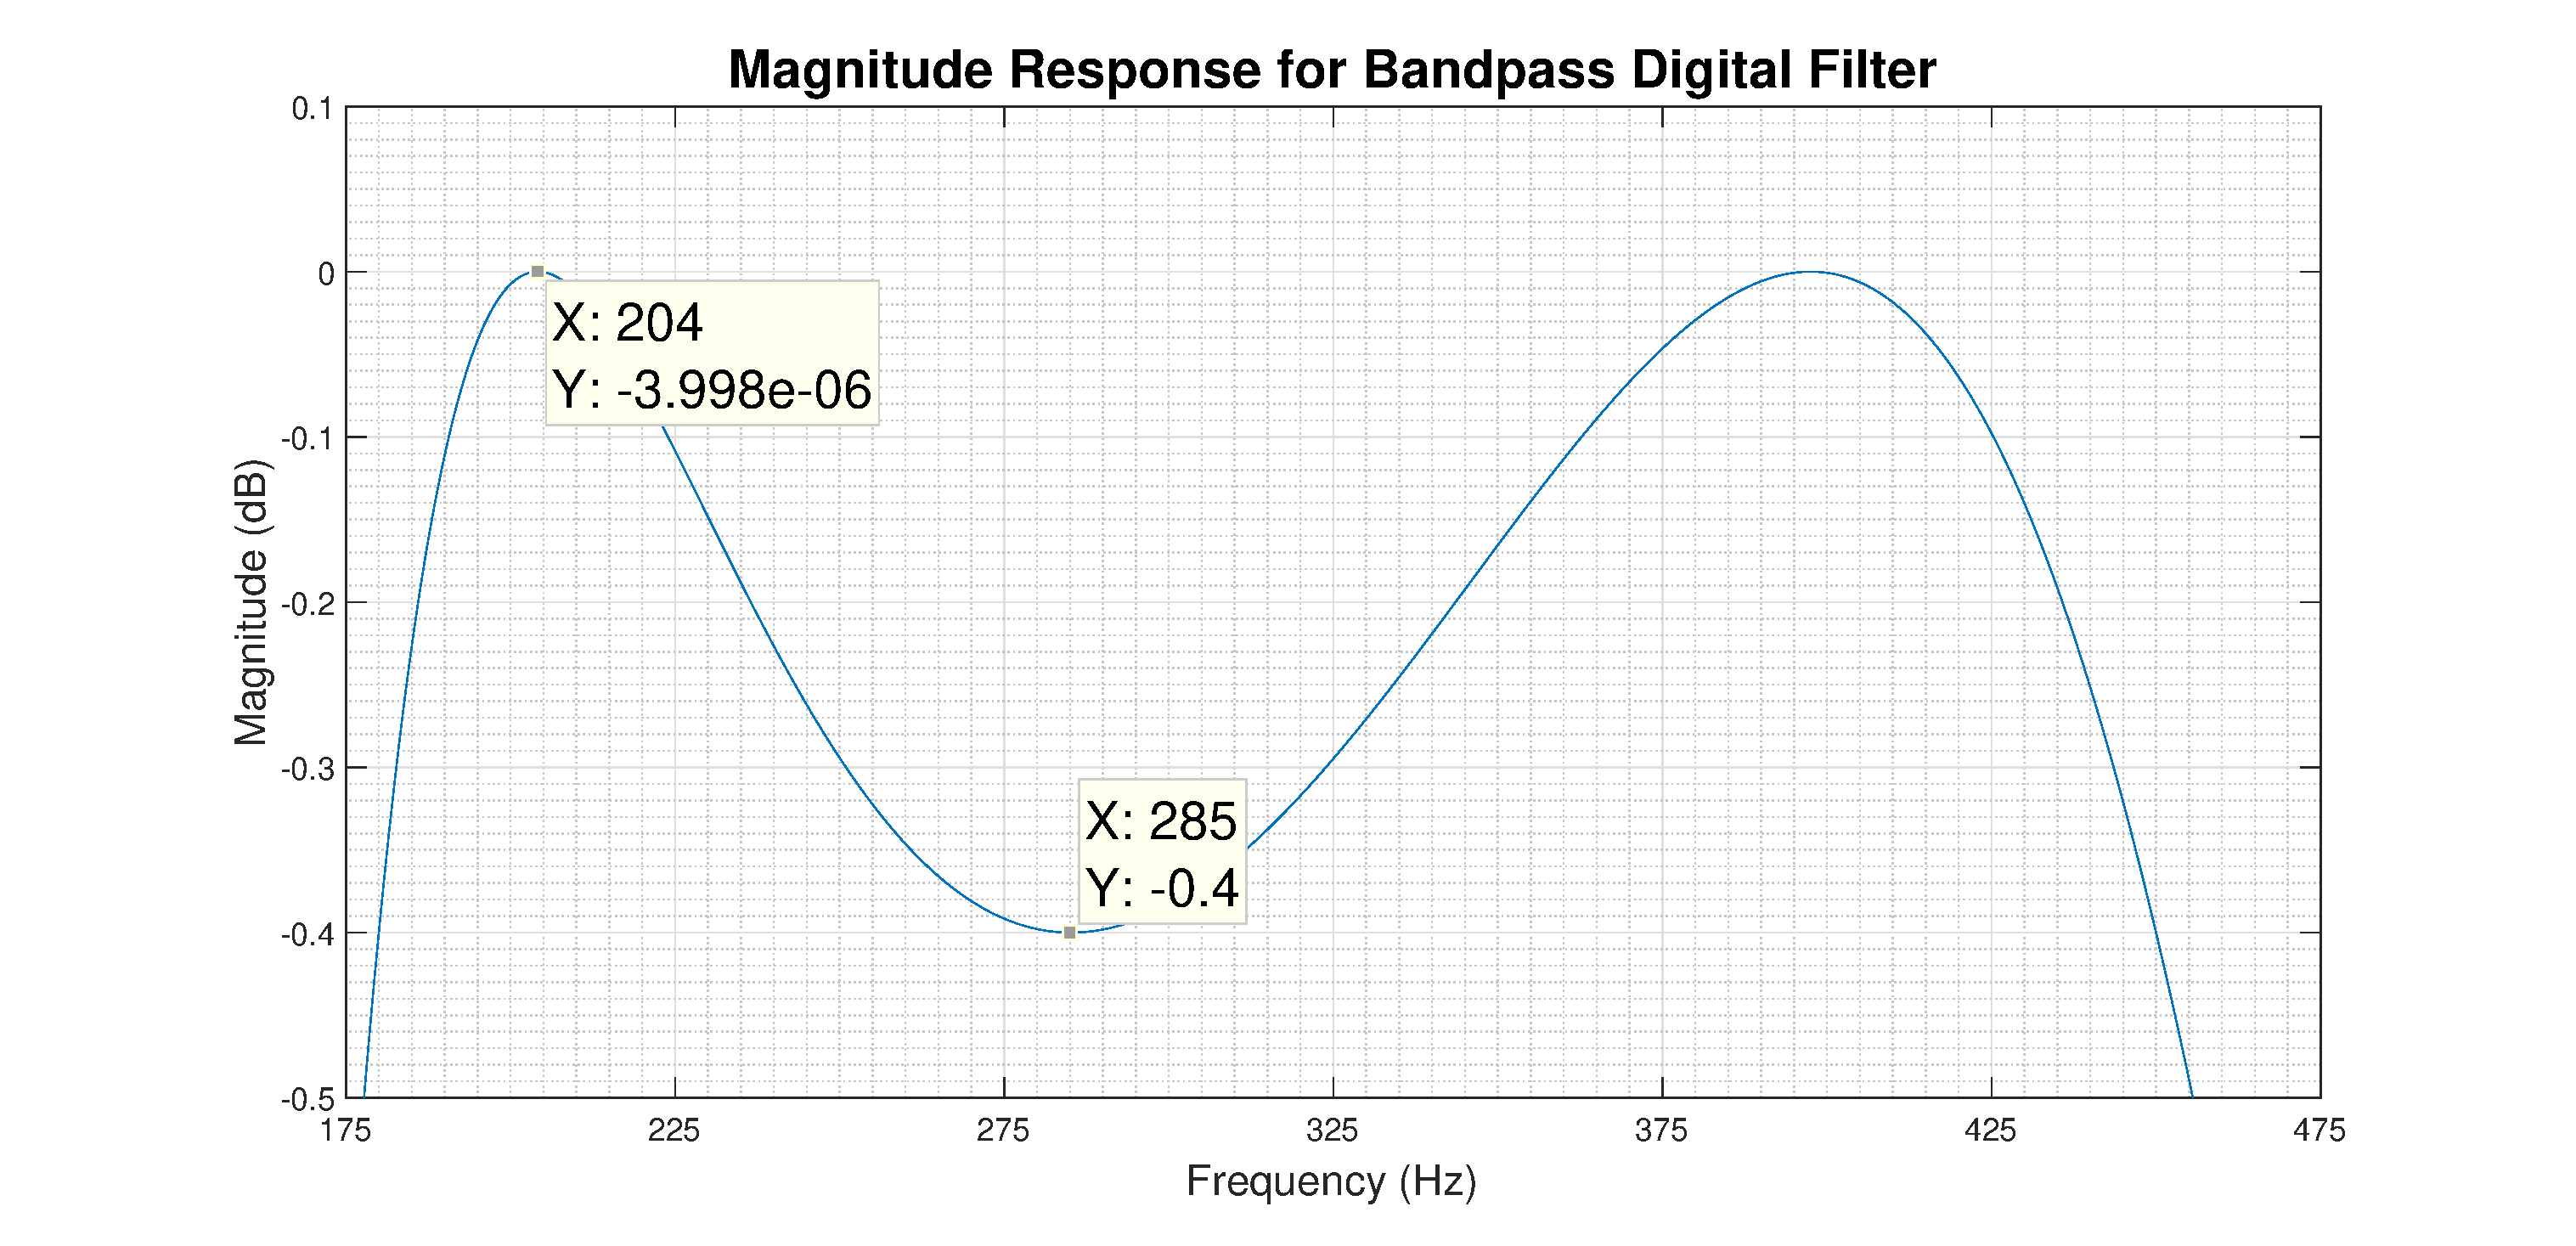
\includegraphics[width = 0.32\textwidth]{mag_response_digital_filter_passband_zoom}
    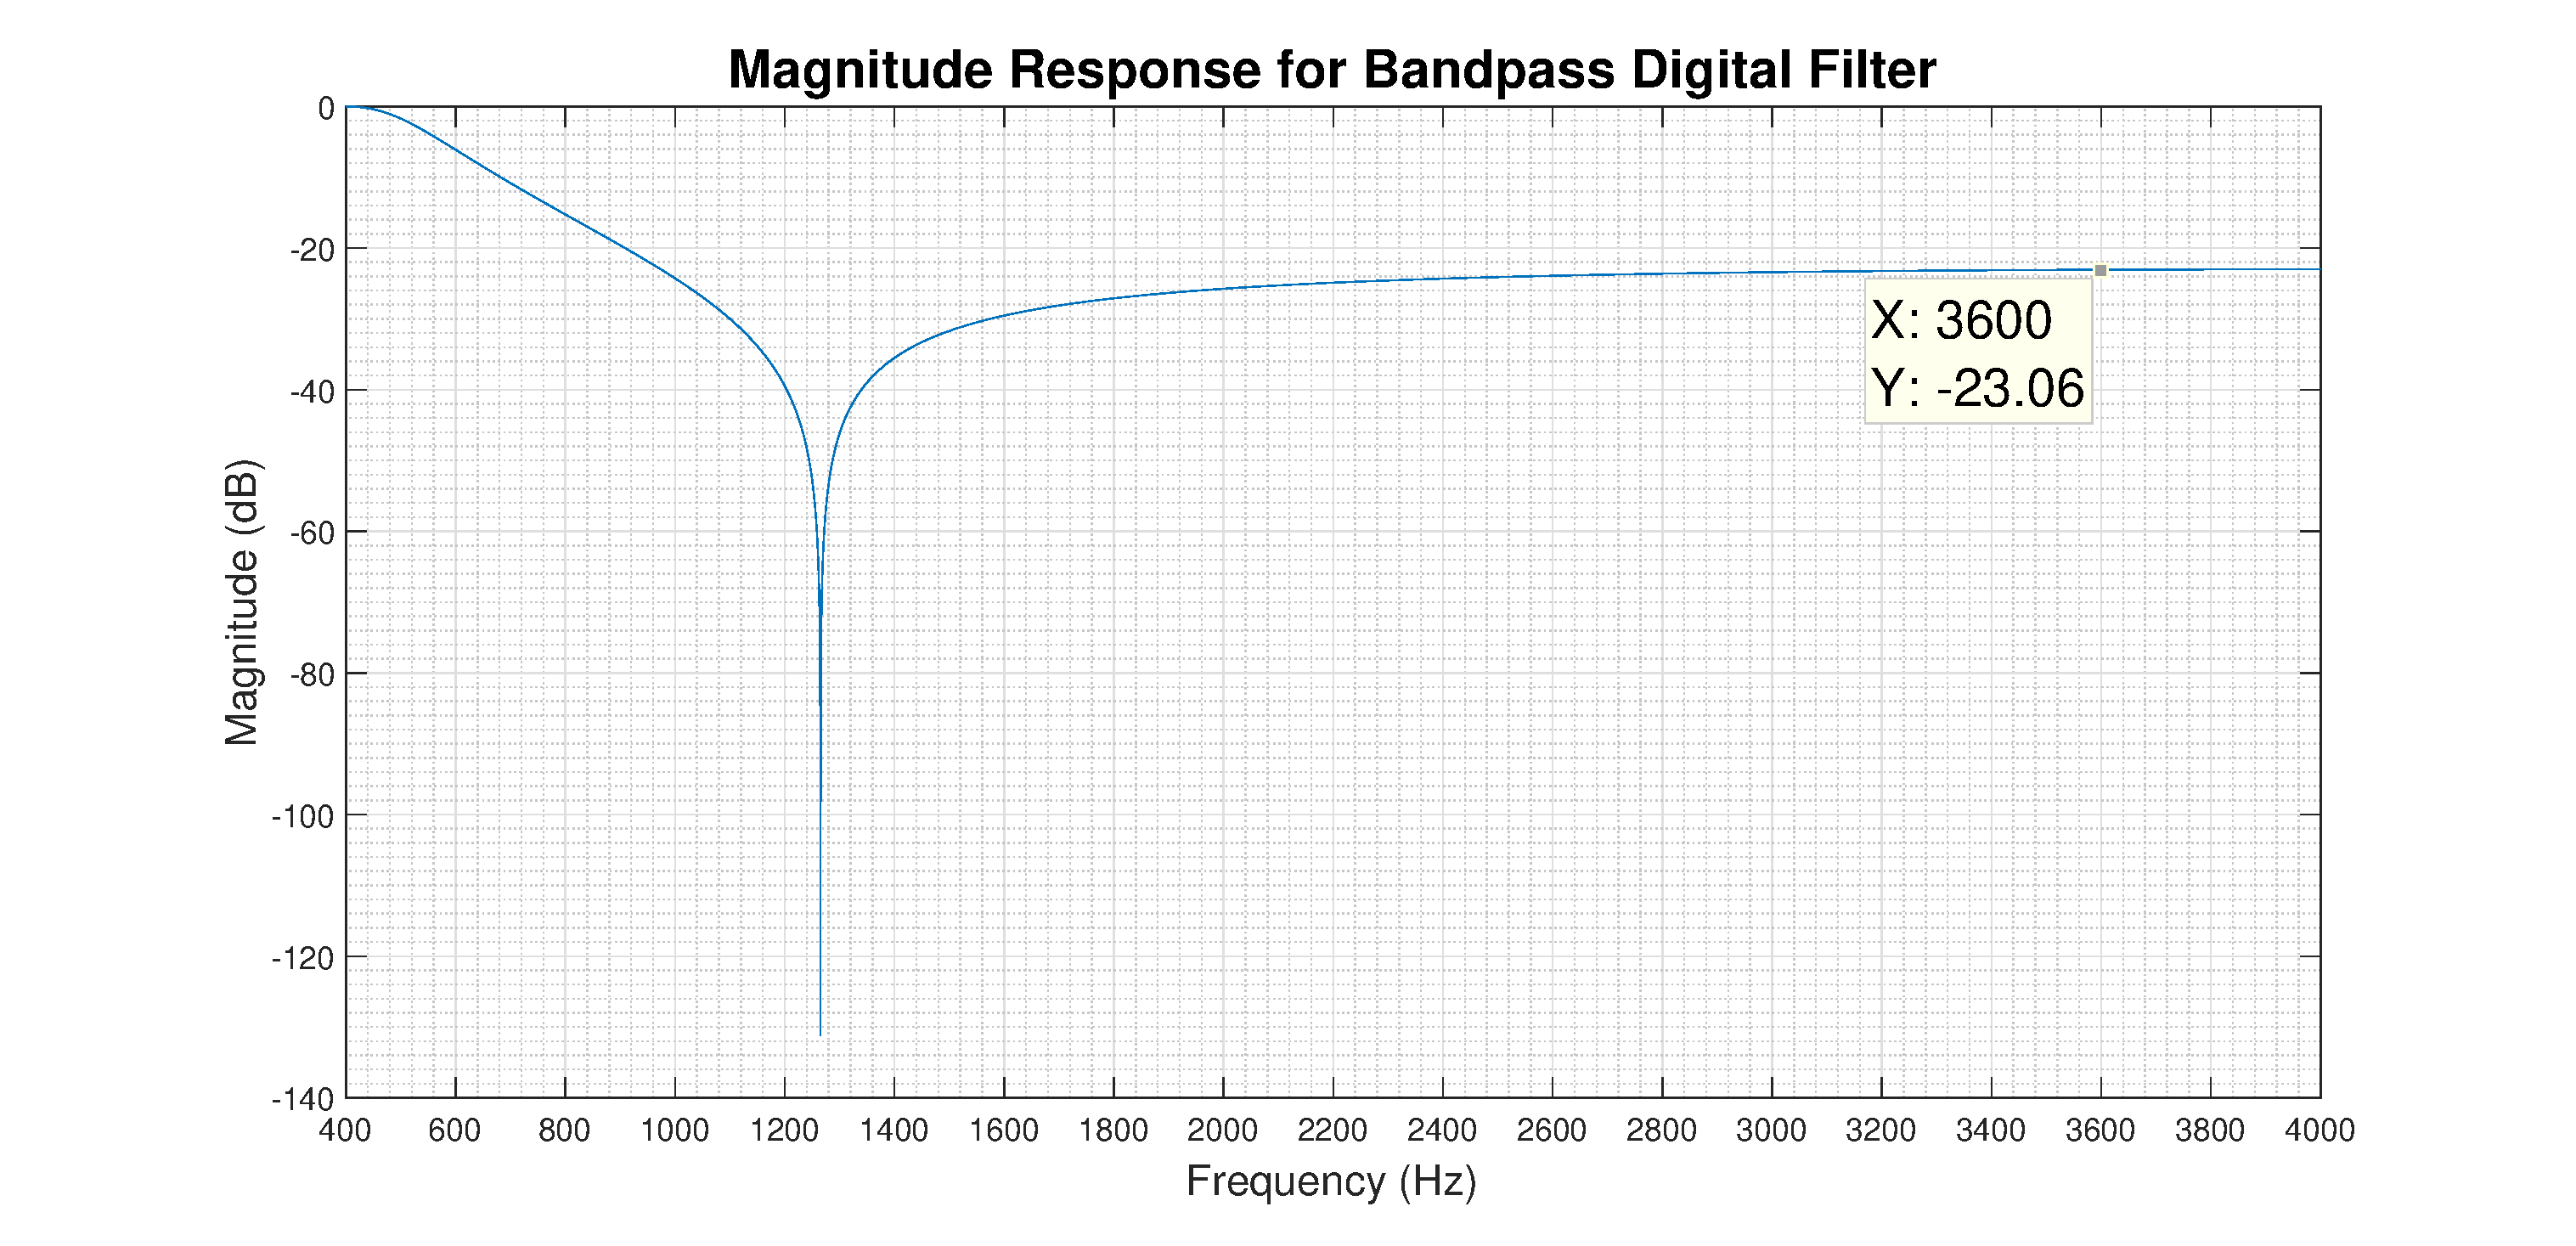
\includegraphics[width = 0.32\textwidth]{mag_response_digital_filter_stopband_right}
    \caption{Theoretical pass band and stop band frequency response of filter designed on MATLAB}
    \label{fig:passband_zoom}
\end{figure}

\newpage
\section{Implementation of Bandpass Filter: Direct Form II Realisation}\label{sec:direct_form_II}
An IIR filter can be implemented in multiple ways. The filter designed in section \ref{sec:bandpass_design} will be implemented using the direct form II realisation. Before the filter can be implemented in C, it is important to understand how the output is calculated.\\

The signal flow graph for the direct form II realisation of an IIR is shown in figure \ref{fig:iir_direct_form_II}. For simplicity, a $3^{rd}$ order system is considered.


\begin{figure}[H]
    \centering
    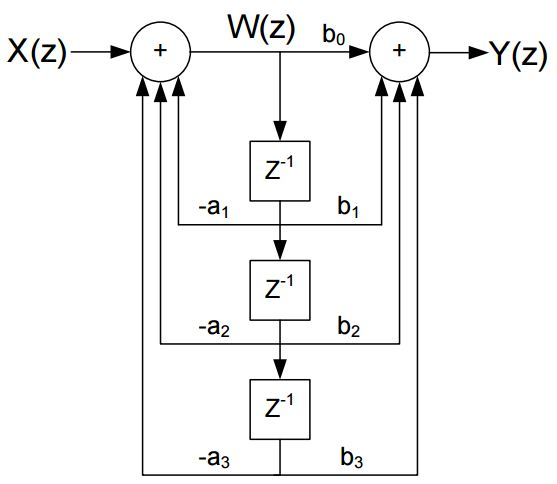
\includegraphics[width = 0.3\textwidth]{iir_direct_form_II}
    \caption{Direct form II realisation of an IIR filter}
    \label{fig:iir_direct_form_II}
\end{figure}

The direct form II realisation of a $3^{rd}$ order IIR filter can be mathematically expressed in equations (\ref{eq:IIR_direct_form_II_1}) and (\ref{eq:IIR_direct_form_II_2}).

\begin{align}
    w(n) &= x(n) - a_{1}x(n-1) - a_{2}x(n-2) - a_{3}x(n-3) \label{eq:IIR_direct_form_II_1}\\
    y(n) &= b_{0}w(n) + b_{1}w(n-1) + b_{2}w(n-2) + b_{3}x(n-3) \label{eq:IIR_direct_form_II_2}
\end{align}

\textbf{The equations above show that the direct form II structure requires computing two variables, $w$ and $y$ through multiply accumulate operations. These are however largely independent and thus parallelism can be employed.} \\

The C code to implement the direct form II realisation of the IIR filter is presented in listing \ref{lst:direct_form_II}. 

\begin{listing}[H]
\begin{minted}[fontsize=\scriptsize,linenos]{C}
void ISR_filter(void){
    // read sample from the line input				
    short sample = mono_read_16Bit();
    
    // compute the next output sample using the designed filter
    double output = direct_form_2(sample);
    
    // write output to the line output
    mono_write_16Bit((short)output);
}

// Function to implement an IIR filter using the Direct Form II realisation
// Function uses a simple buffer
double direct_form_2(short sample){

    // declare variable for loops 
    int i;
    
    // declare variable to store output
    double output = 0;
    
    // x[0] will contain (after for loop): sample minus all 'a' coefficient terms
    x[0] = sample;
    
    for (i = N; i > 0; i--){
        x[0] -= a[i]*x[i];      // accumulate 'a' coefficient terms
        output += b[i]*x[i];    // accumulate 'b' coefficient terms
        x[i] = x[i-1];          // shift the buffer along
    }
    
    // compute output by summing the accumulation of 'a' coefficients (stored in x[0])
    // and 'b' coefficients (already stored in output)
    output += b[0]*x[0];
    
    return(output);
}
\end{minted}
\caption{{\tt direct\_form\_2}} 
\label{lst:direct_form_II}
\end{listing}

The function {\tt direct\_form\_2} utilises a simple buffer. The memory required for the buffer is dynamically allocated using the {\tt calloc} function. The {\tt calloc} function initialises the buffer elements to $0$, and thus zeroing is not required. \textbf{ The simple buffer requires a great deal of overhead to maintain because complete reorganisation of the buffer, each time a new sample is read, is required. The simple buffer however can be implemented very easily in C.}\\

\textbf{As discussed in the previous report, the use of a circular buffer can significantly improve performance.} Complete reorganisation of the buffer is no longer required. A pointer is used to signify at which point in the array the newest sample is currently stored. The pointer is wrapped around when the end of the array is reached. Moreover, by doubling the size of the buffer, the use of {\tt if} statements, likely to cause pipeline stalls, can be eliminated. With a double sized buffer, there is no danger of overflow in the {\tt for} loop.\\

\textbf{As such, the code presented in listing \ref{lst:direct_form_2_circ} utilises a double sized circular buffer. The function {\tt direct\_form\_2\_circ} also utilises pointers to improve performance.} In the previous report, it was established that the use of pointers can be used to improve performance. In assembly, pointers can be referenced and incremented/decremented in one instruction. Optimisation level 2 seeks to optimise code to use pointer automatically however often the compiler is not able to identify areas where such optimisation can be utilised. As such, pointers are used explicitly in the function {\tt direct\_form\_2\_circ}. \\ 

\begin{listing}[H]
\begin{minted}[fontsize=\scriptsize,linenos]{C}
void ISR_filter(void){
    // read sample from the line input				
    short sample = mono_read_16Bit();
    
    // compute the next output sample using the designed filter
    double output = direct_form_2_circ(sample);
    
    // write output to the line output
    mono_write_16Bit((short)output);
}

// Function to implement an IIR filter using Direct Form II
// Function uses a double-sized circular buffer
// Pointers used for optimisation and code portability
// Requires:
//      GLOBAL: double *index;
//      MAIN:   x = (double *)calloc(2*(N+1), sizeof(double));
//              index = x;

double direct_form_2_circ(short sample){

    // declare variable for for-loop
    int i;
    
    // declare variable to store output
    double output = 0;
    
    // declare pointers for filter coefficients 
    const double *ptr_a = a;
    const double *ptr_b = b;
    
    // *index should contain (after for-loop): sample minus all 'a' coefficient terms
    // update *(index+N+1) to prevent the need for wrap-around in the loop
    *index = *(index+N+1) = sample;
    
    for (i = 1; i <= N; i++){
        *index -= (*(ptr_a+N+1-i) * *(index+i));    // accumulate 'a' coefficient terms
        output += *(index+i) * *(ptr_b+N+1-i);      // accumulate 'b' coefficient terms
    }
    
    // update *(index+N+1)
    *(index+N+1) = *index;
    
    // compute output by summing the accumulation of 'a' coefficients (stored in *index)
    // and 'b' coefficients (already stored in output)
    output += *index * *ptr_b;
    
    // increment buffer pointer
    index++;
    
    // wrap the pointer around if it gets to half the size of the double-buffer
    if(index == &x[N+1])
        index = x;	
    
    return(output);	
}
\end{minted}
\caption{{\tt direct\_form\_2\_circ}} 
\label{lst:direct_form_2_circ}
\end{listing}

\subsection{Direct Form II Realisation: Analysis of Performance}
In order to profile the performance of the direct form II realisation of the IIR filter, the clock cycles required to calculate the output were measured. Breakpoints were inserted after reading the newest sample but before writing the output to the $AIC23$ audio codec. Performance of the algorithm is measured for various orders of filters\footnote{The filter became unstable after order $N=14$. This will be discussed later. Nonetheless, the number of clock cycles was measured.}. The results obtained are presented in table \ref{tab:direct_form_2}.

\begin{table}[H]
  \centering
    \begin{tabular}{|r|c|c|c|c|}
\cline{2-5}    \multicolumn{1}{r|}{} & \multicolumn{2}{c|}{{\tt direct\_form\_2}} & \multicolumn{2}{c|}{{\tt direct\_form\_2\_circular}} \\
    \hline
    \multicolumn{1}{|c|}{Order} & No Optimisation & Level 2 & No Optimisation & Level 2 \\
    \hline
    \multicolumn{1}{|c|}{2} & 135 & 112 & 170 & 129 \\
    \hline
    \multicolumn{1}{|c|}{4} & 245 & 177   & 250 & 181 \\
    \hline
    \multicolumn{1}{|c|}{6} & 356   & 241 & 330 & 232 \\
    \hline
    \multicolumn{1}{|c|}{8} & 466 & 306 & 411   & 284 \\
    \hline
    \multicolumn{1}{|c|}{10} & 576 & 370 & 491 & 335 \\
    \hline
    \multicolumn{1}{|c|}{12} & 686 & 435 & 571 & 387 \\
    \hline
    \multicolumn{1}{|c|}{14} & 796 & 500   & 651 & 439 \\
    \hline
    \multicolumn{1}{|c|}{16} & 907   & 564 & 731 & 490 \\
    \hline
    \multicolumn{1}{|c|}{18} & 1017 & 629 & 812   & 542 \\
    \hline
    \multicolumn{1}{|c|}{20} & 1127 & 693 & 892 & 593 \\
    \hline
    \end{tabular}%
    \caption{Direct form II performance}
  \label{tab:direct_form_2}%
\end{table}%


Figure \ref{fig:direct_form_2_performance} maps the performance of the two functions {\tt direct\_form\_2} and {\tt direct\_form\_2\_circ}.

\begin{figure}[H]
    \centering
    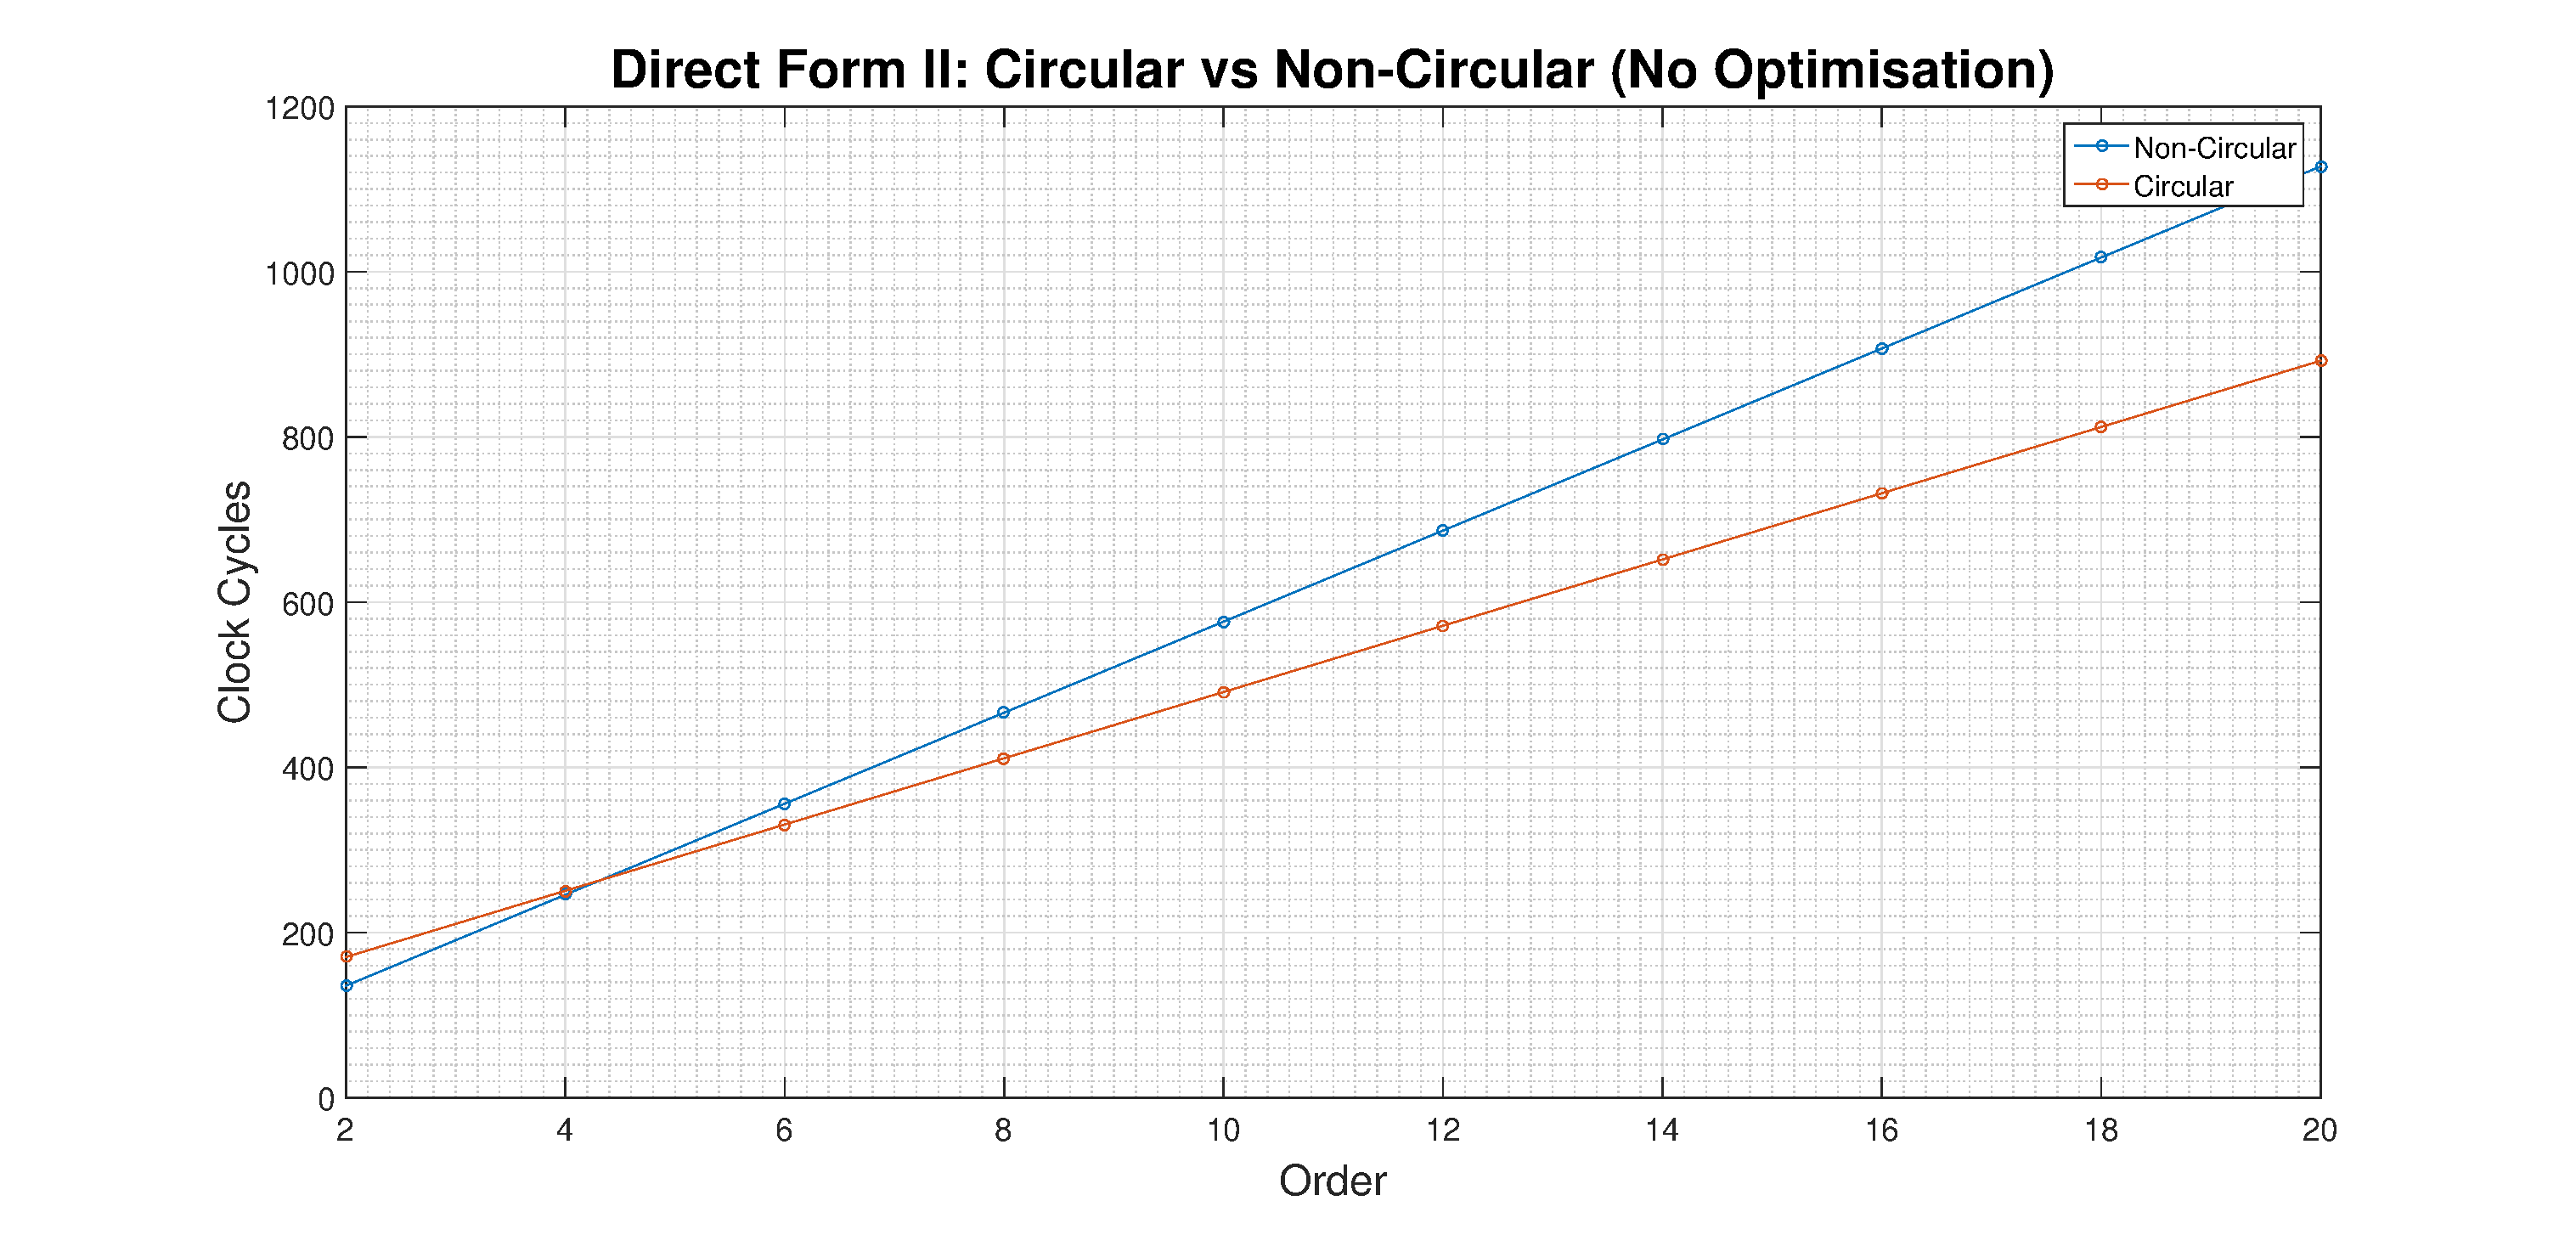
\includegraphics[width = 0.70\textwidth]{direct_form_2_no_opt}
    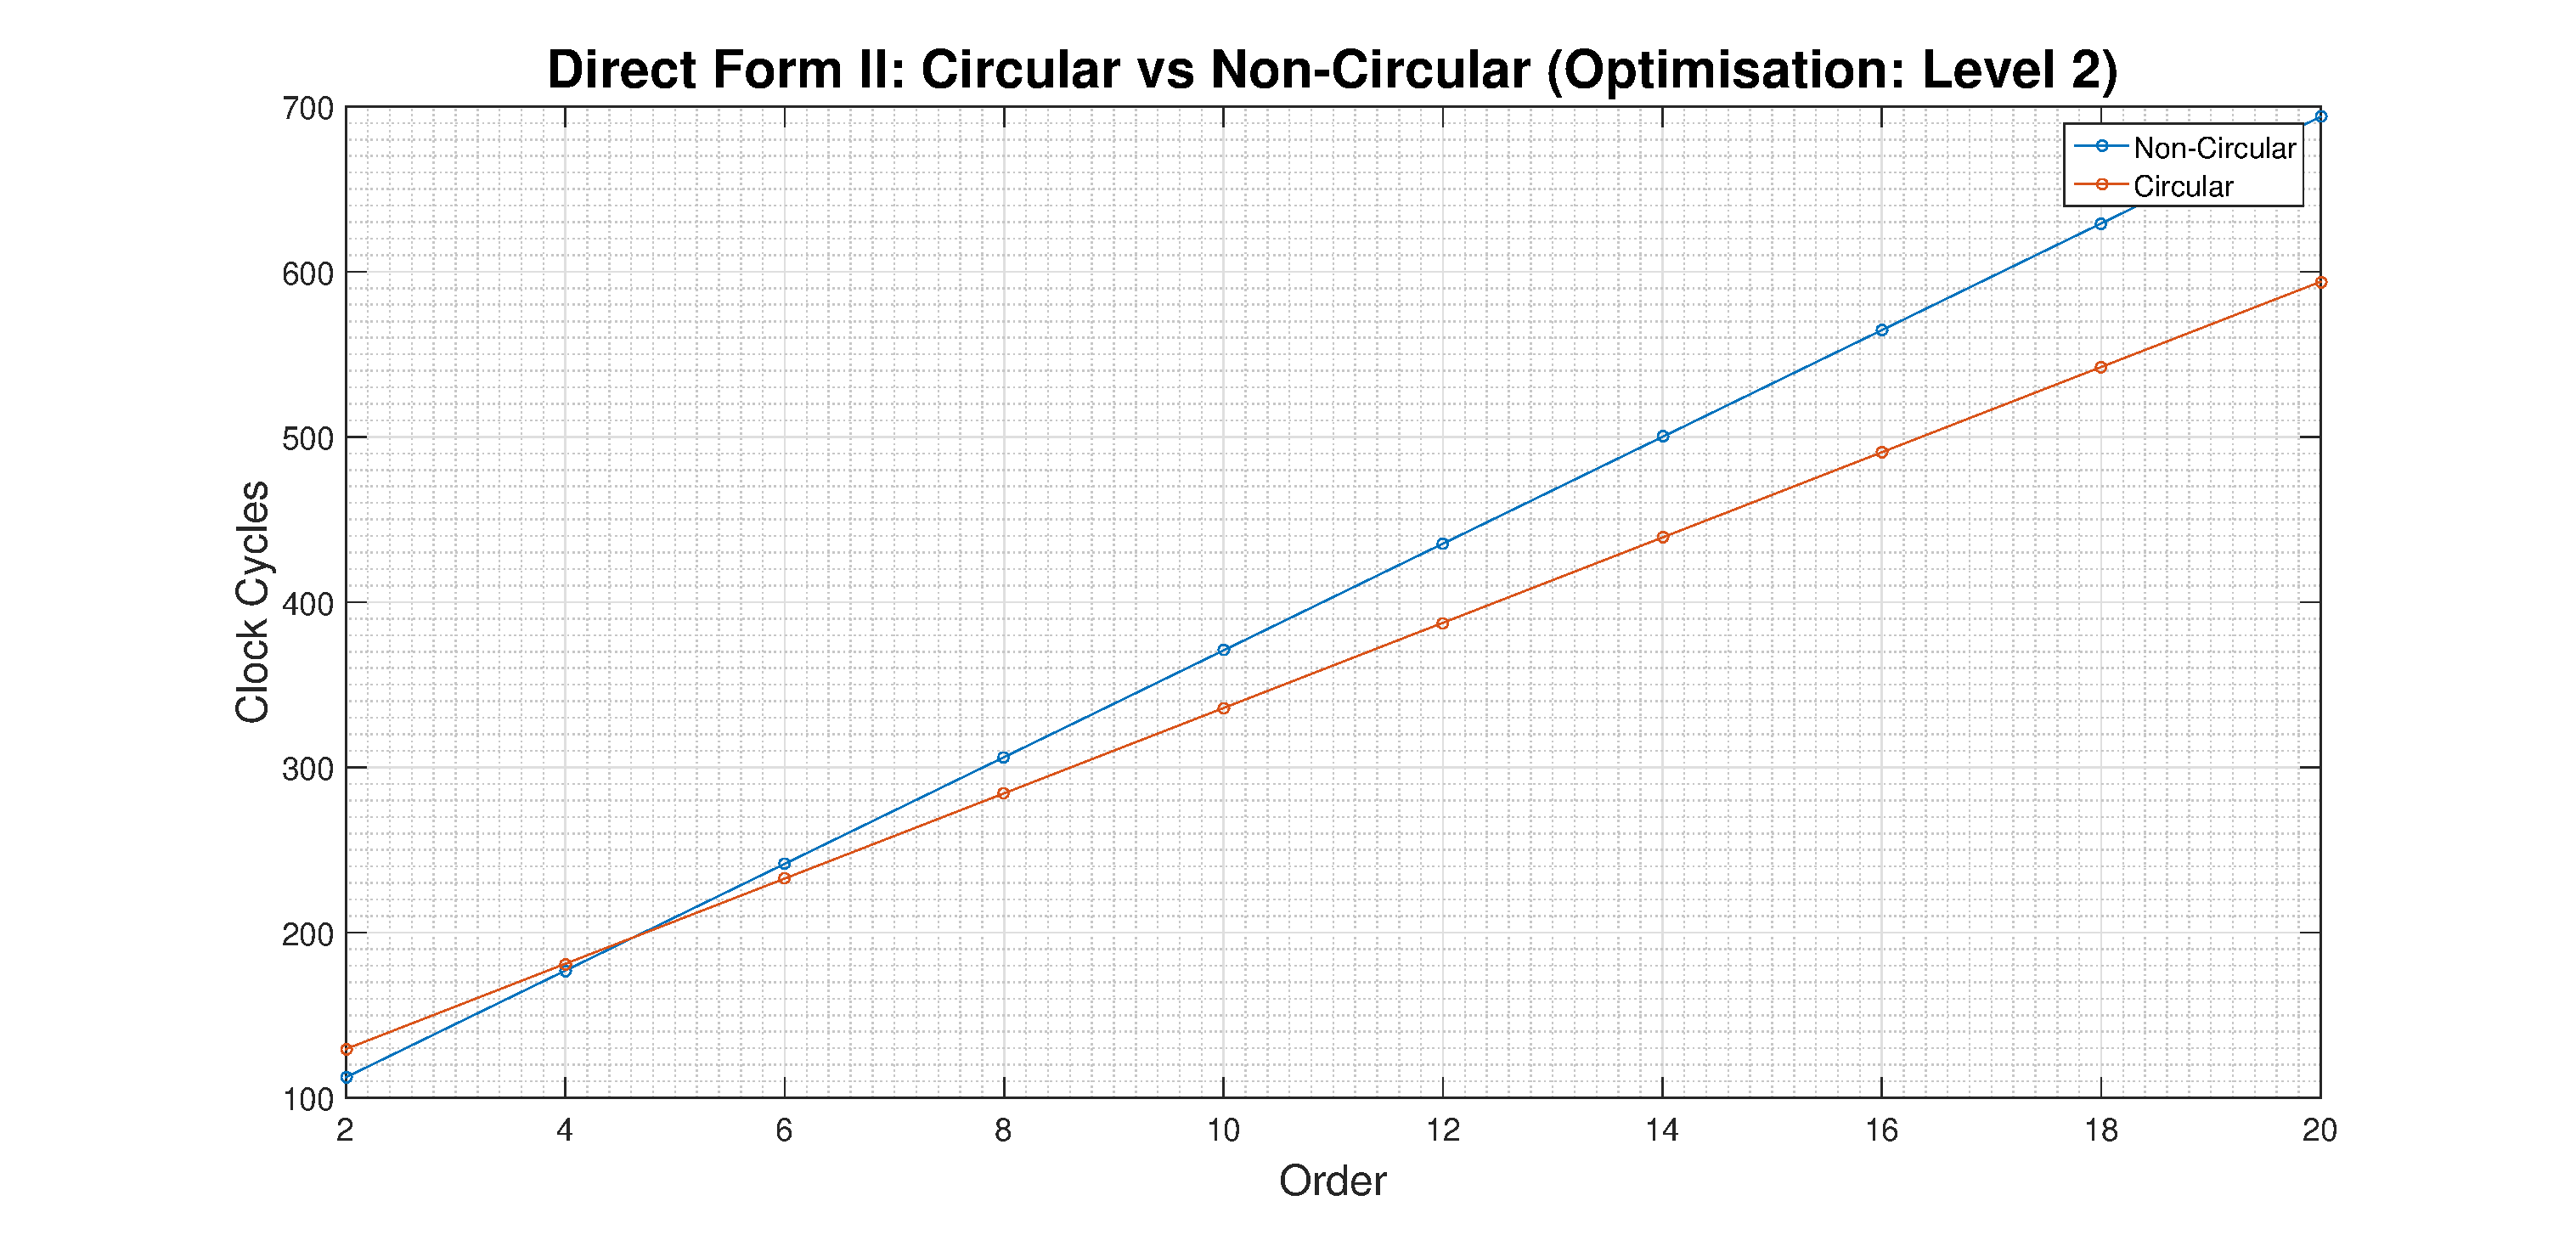
\includegraphics[width = 0.70\textwidth]{direct_form_2_opt}
    \caption{Performance of direct form II realisation of IIR filter}
    \label{fig:direct_form_2_performance}
\end{figure}


\textbf{From the data obtained, it is evident that the implementation of the circular buffer significantly improves the performance of the filtering process. Using a circular buffer requires half the number of memory access operations than if a simple buffer was used. As such, the circular buffer implementation is expected to be significantly faster.}\\

\textbf{This is however not true when small filter orders are utilised. When a $2^{nd}$ order filter is used, both functions require similar number of memory access operations however the circular buffer implementation requires more calculations outside the {\tt for} loop. This includes the {\tt if} statement required to implement the wrapping around and other calculations required to determine the buffer location that the newest sample has to be written to. When a $4^{th}$ order filter is implemented, even though the circular buffer implementation requires less memory access operations than the simple buffer implementation, the overhead required to maintain the circular buffer still results in the simple buffer implementation being slightly faster.} \\

\textbf{The clear benefits of utilising a circular buffer become obvious when filters of order greater than 4 are implemented.} This can be understood mathematically from equations (\ref{eq:non_circ_time}) and (\ref{eq:circular_time}). The circular buffer implementation has a smaller gradient than the non circular buffer and thus scales better with filter order. However its y-intercept is significantly larger. The large y-intercept accounts for the slow performance at small filter orders. 

\begin{align}
    T_{Non-Circular} = 55.1N + 25.4 \label{eq:non_circ_time}\\
    T_{Circular} = 40.1N +90.2\label{eq:circular_time}
\end{align}

When compiler optimisation is utilised, the performance of both functions increases. This is exactly as expected. The increase in performance is more significant at higher orders. This is also exactly as expected. \textbf{The optimisation requires rearranging of the {\tt for} loop and this has some overhead. However, once the rearrangement of the {\tt for} loop has been completed, arbitrarily increasing the order of the filter does not present a significant increase in the number of clock cycles required.} Once again, this can be understood mathematically; the gradient of both the circular and the non circular implementation has decreased.

\begin{align}
    T_{Non-Circular,\ Optimisation} = 32.3N + 47.8 \label{eq:non_circ_time}\\
    T_{Circular,\ Optimisation} = 25.8N +77.9\label{eq:circular_time}
\end{align}


\newpage
\section{Implementation of Bandpass Filter: Direct Form II Transposed}
An discussed in section \ref{sec:direct_form_II}, an IIR filter can be implemented in multiple ways. The filter designed in section \ref{sec:bandpass_design} will now be implemented using the transposed form realisation. Before the filter can be implemented in C, it is important to understand how the output is calculated.\\

The signal flow graph for the transposed form realisation of an IIR is shown in figure \ref{fig:iir_transposed_form_II}.

\begin{figure}[H]
    \centering
    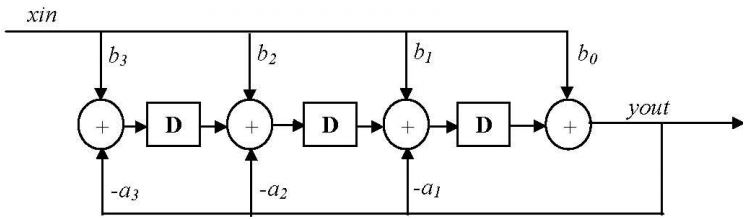
\includegraphics[width = 0.6\textwidth]{Direct_Form_2_transposed}
    \caption{Direct form II transposed realisation of an IIR filter}
    \label{fig:iir_transposed_form_II}
\end{figure}

\textbf{The first thing to notice is that the transpose form explicitly reveals the recursive nature of IIR filters.} In section \ref{sec:IIR_filter}, it was highlighted that an IIR filter has infinite memory. This is implemented by feeding the output back into the system. In the direct form II realisation, this feedback was less explicit.\\

\textbf{Note that the transposed form realisation of an IIR filter is expected to perform faster than the direct form II realisation explored in section \ref{sec:direct_form_II}. Although the transposed form does not allow for parallelised computations like the direct form II, the transposed form algorithm does not require excessive shifting of samples within the buffer. The buffer is updated continuously with intermediate values that are calculated. Elements in the buffer are overwritten not shifted.} The code to implement the transposed form realisation of the IIR filter designed in section \ref{sec:design_of_digital_filter} is presented in listing \ref{lst:transposed_form}.

\begin{listing}[H]
\begin{minted}[fontsize=\scriptsize,linenos]{C}
void ISR_filter(void){
    // read sample from the line input				
    short sample = mono_read_16Bit();
    
    // compute the next output sample using the designed filter
    double output = transposed_form(sample);
    
    // write output to the line output
    mono_write_16Bit((short)output);
}

// Function to implement an IIR filter using Transposed Form
// Buffer size is equivalent to order of filter
// 1 less element in the buffer as compared to direct form II implementation
// Pointers used for optimisation and code portability
// Requires:
//      GLOBAL: double *index;
//      MAIN:   x = (double *)calloc(N, sizeof(double));
//              index = x;

double transposed_form(const short sample){
    
    // declare variable for for-loop
    int i;
    
    // declare pointers for filter coefficients 
    const double *ptr_a = &a[1];
    const double *ptr_b = &b[1];
    
    // declare variable to store output
    const double output =  b[0]*sample + x[0];
    
    // compute next buffer values for the next function call
    for (i = 0; i < N-1; i++){
        x[i] = x[i+1] + *(ptr_b++)*sample - *(ptr_a++)*output;
    }
    
    x[N-1] = *(ptr_b)*sample - *(ptr_a)*output;
    
    return(output);	
}

\end{minted}
\caption{{\tt transposed\_form}} 
\label{lst:transposed_form}
\end{listing}

\textbf{After a new sample is read, it is stored in a temporary variable called {\tt sample}. It is important to note that the buffer {\tt x} in the transformed form realisation does not contain past input samples. The buffer holds intermediate values that will be used to calculate the output. The intermediate values that are to be held in the buffer are calculated within the {\tt for} loop. Notice that the last element in the buffer is calculated outside the {\tt for} loop because it's mathematical structure is different from the other elements.}\\

Note that the compiler deals very well with variables defined as {\tt const}. They have been utilised to improve code performance 

\subsection{Transposed Form Realisation: Analysis of Performance}

As in the case of the direct form II filter, the performance of the transposed form realisation will be analysed and a relationship will be obtained in the form $A+BN$.\\

Table \ref{tab:trans_form} provides the data obtained when the transposed form filter was run on the $DSK$ board. 

\begin{table}[H]
  \centering
    \begin{tabular}{|c|c|c|}
\cline{2-3}    \multicolumn{1}{c|}{} & \multicolumn{2}{c|}{{\tt transposed\_form} } \\
    \hline
    Order & No Optimisation & Level 2 \\
    \hline
    2     & 101 & 103 \\
    \hline
    4     & 162 & 144 \\
    \hline
    6     & 224 & 185 \\
    \hline
    8     & 285 & 227 \\
    \hline
    10    & 347 & 268 \\
    \hline
    12    & 408 & 309 \\
    \hline
    14    & 469 & 350 \\
    \hline
    16    & 531 & 391 \\
    \hline
    18    & 592 & 433 \\
    \hline
    20    & 654 & 474 \\
    \hline
    \end{tabular}%
  \caption{Transposed form performance}
  \label{tab:trans_form}%
\end{table}%

From the data presented in table \ref{tab:trans_form}, equations (\ref{eq:trans_no_opt}) and (\ref{eq:trans_opt}) are obtained. It is evident that optimisation decreased the gradient of the slope and thus the algorithm scales better when the filter order is increased.

\begin{align}
    T_{Transposed,\  No \ Optimisation} &= 30.7N + 40.0 \label{eq:trans_no_opt}\\
    T_{Transposed,\  Optimisation} &= 20.6N + 62.2 \label{eq:trans_opt}
\end{align} 

Figure \ref{fig:trans_form} presents the data obtained in table \ref{tab:trans_form} graphically. 

\begin{figure}[H]
    \centering
    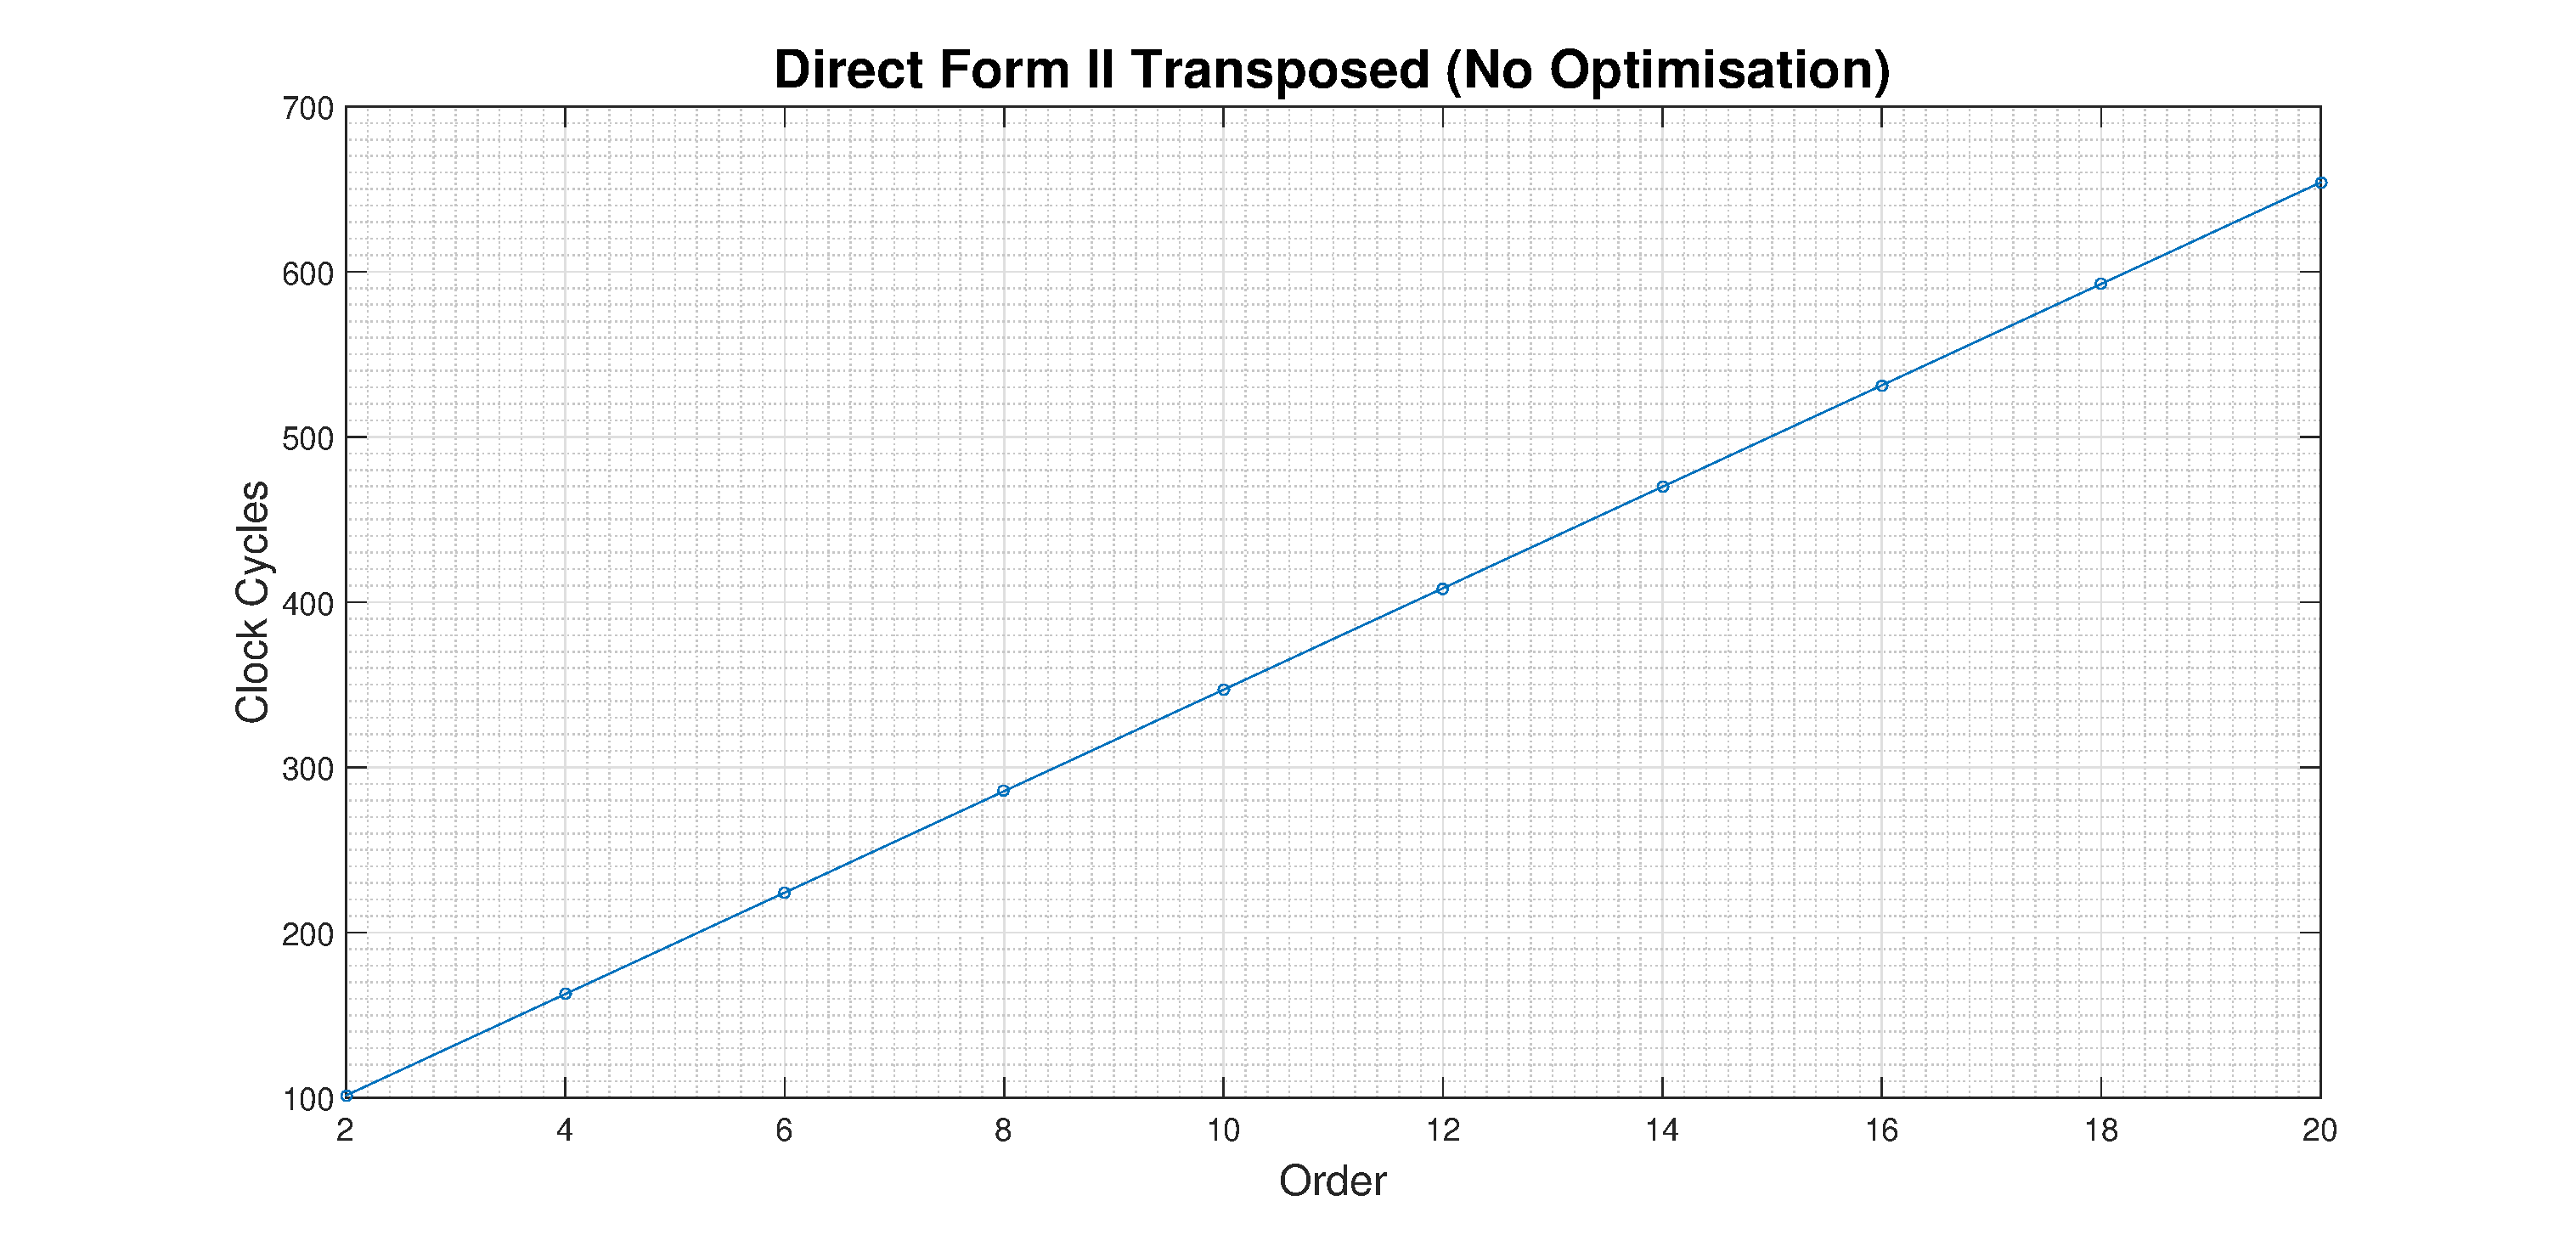
\includegraphics[width = 0.49\textwidth]{trans_no_opt}
    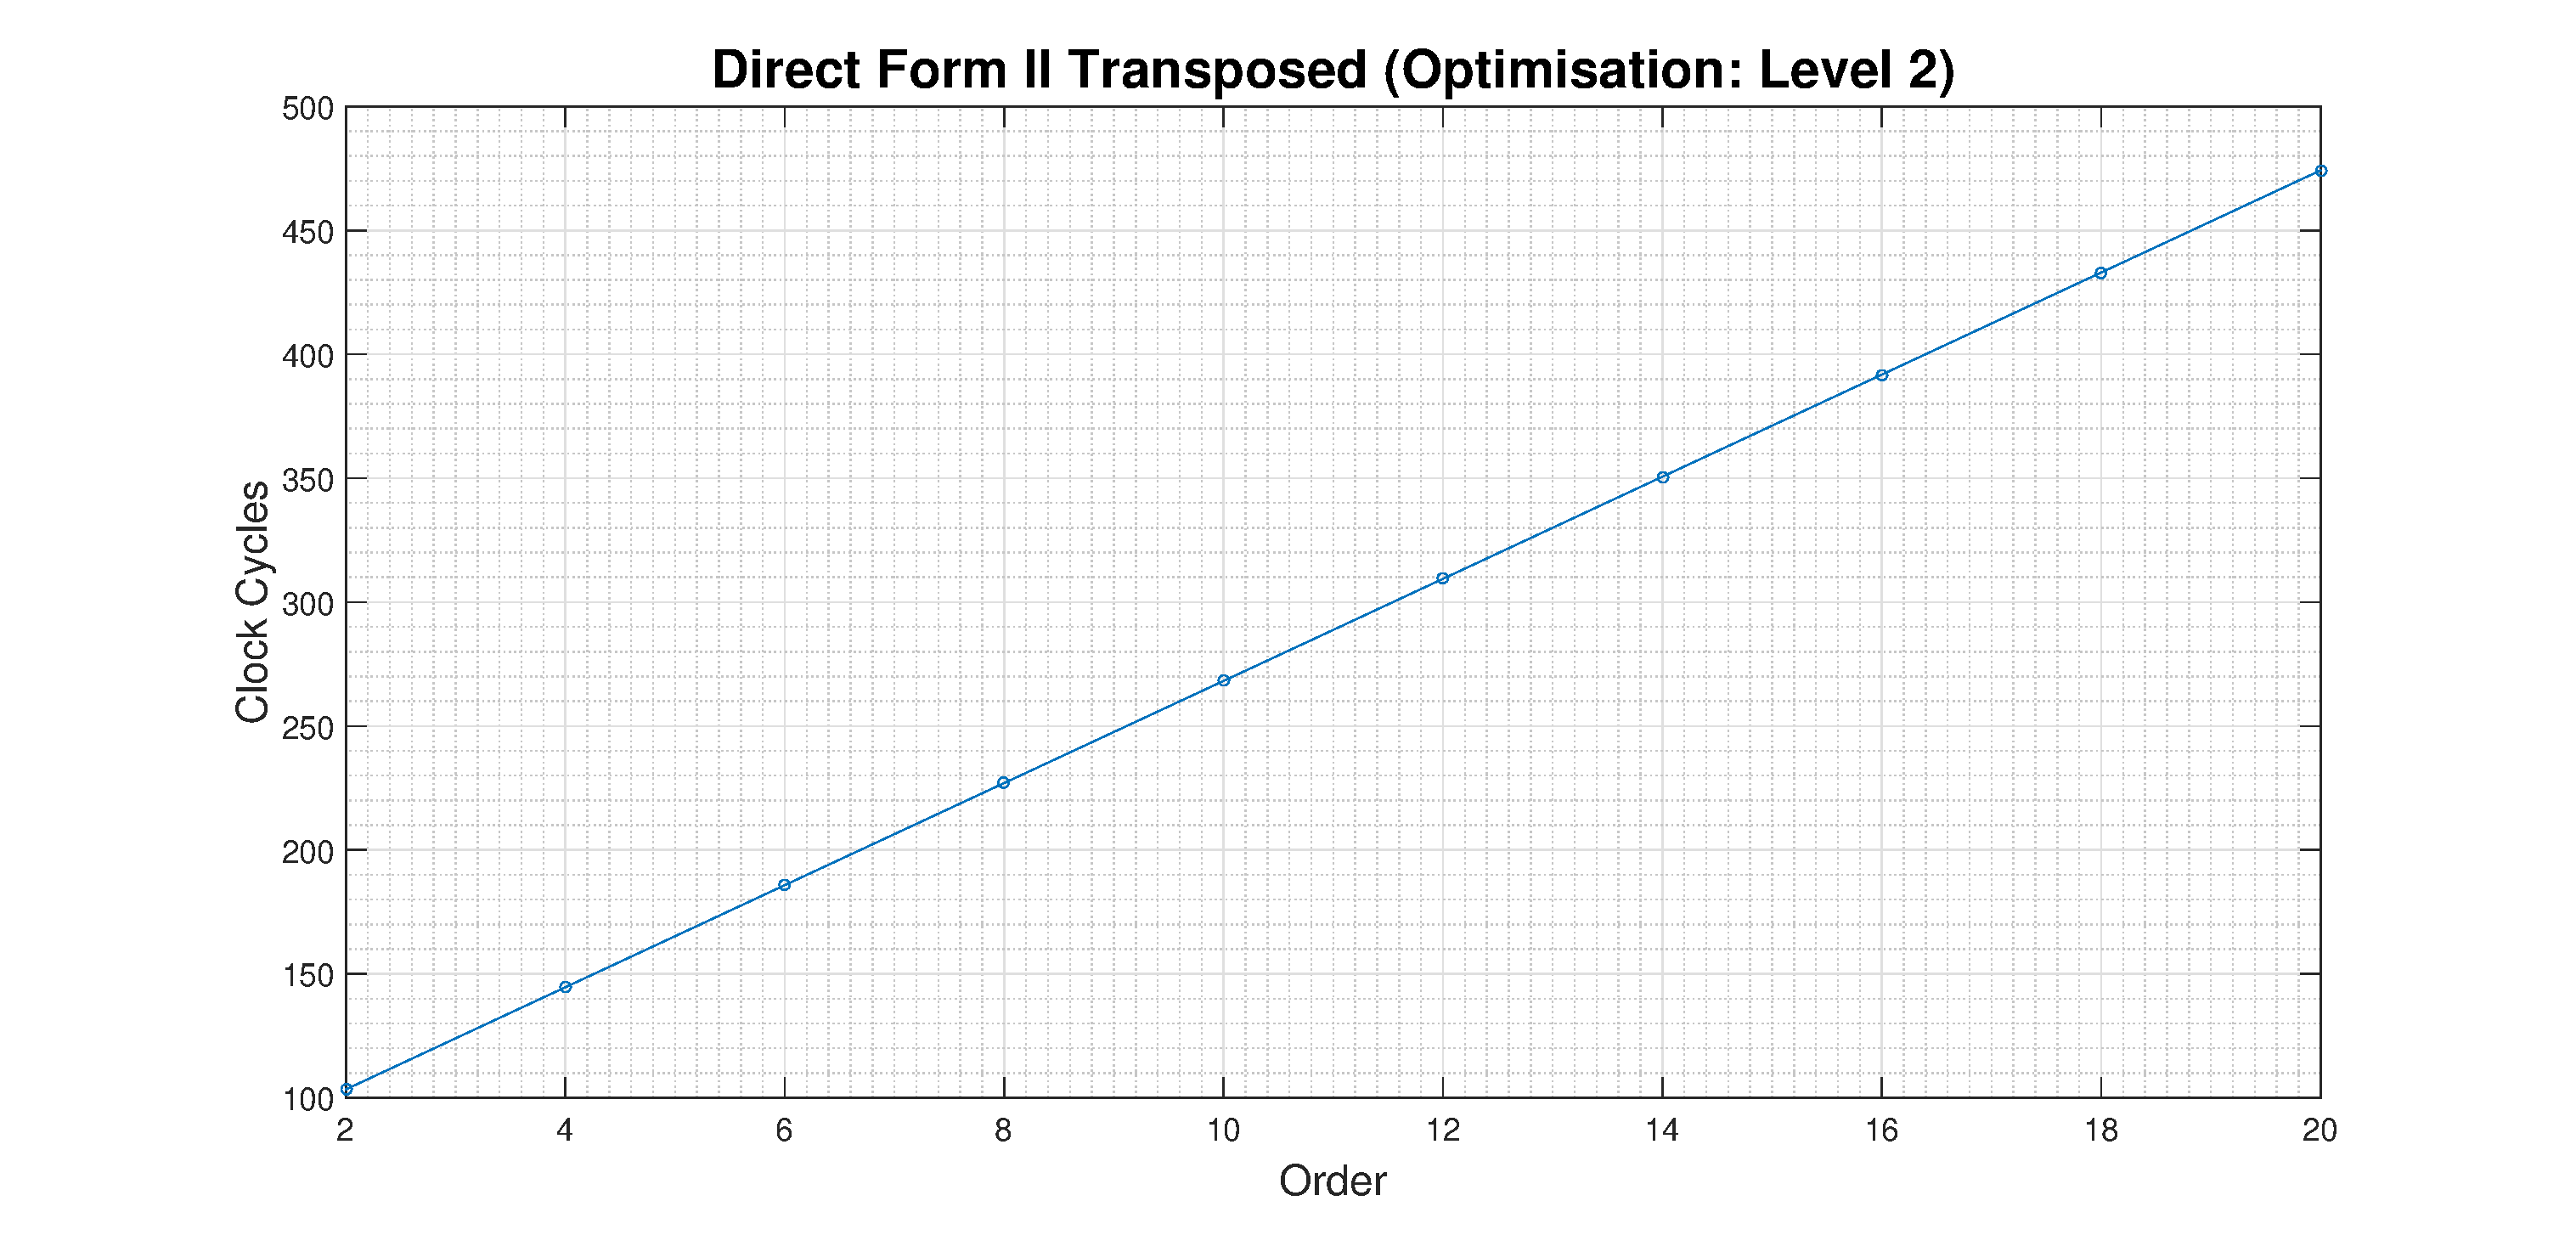
\includegraphics[width = 0.49\textwidth]{trans_opt}
    \caption{Performance of transposed form realisation of IIR filter}
    \label{fig:trans_form}
\end{figure}

\section{Comparison of Direct Form II and Transposed Form}

\begin{figure}[H]
    \centering
    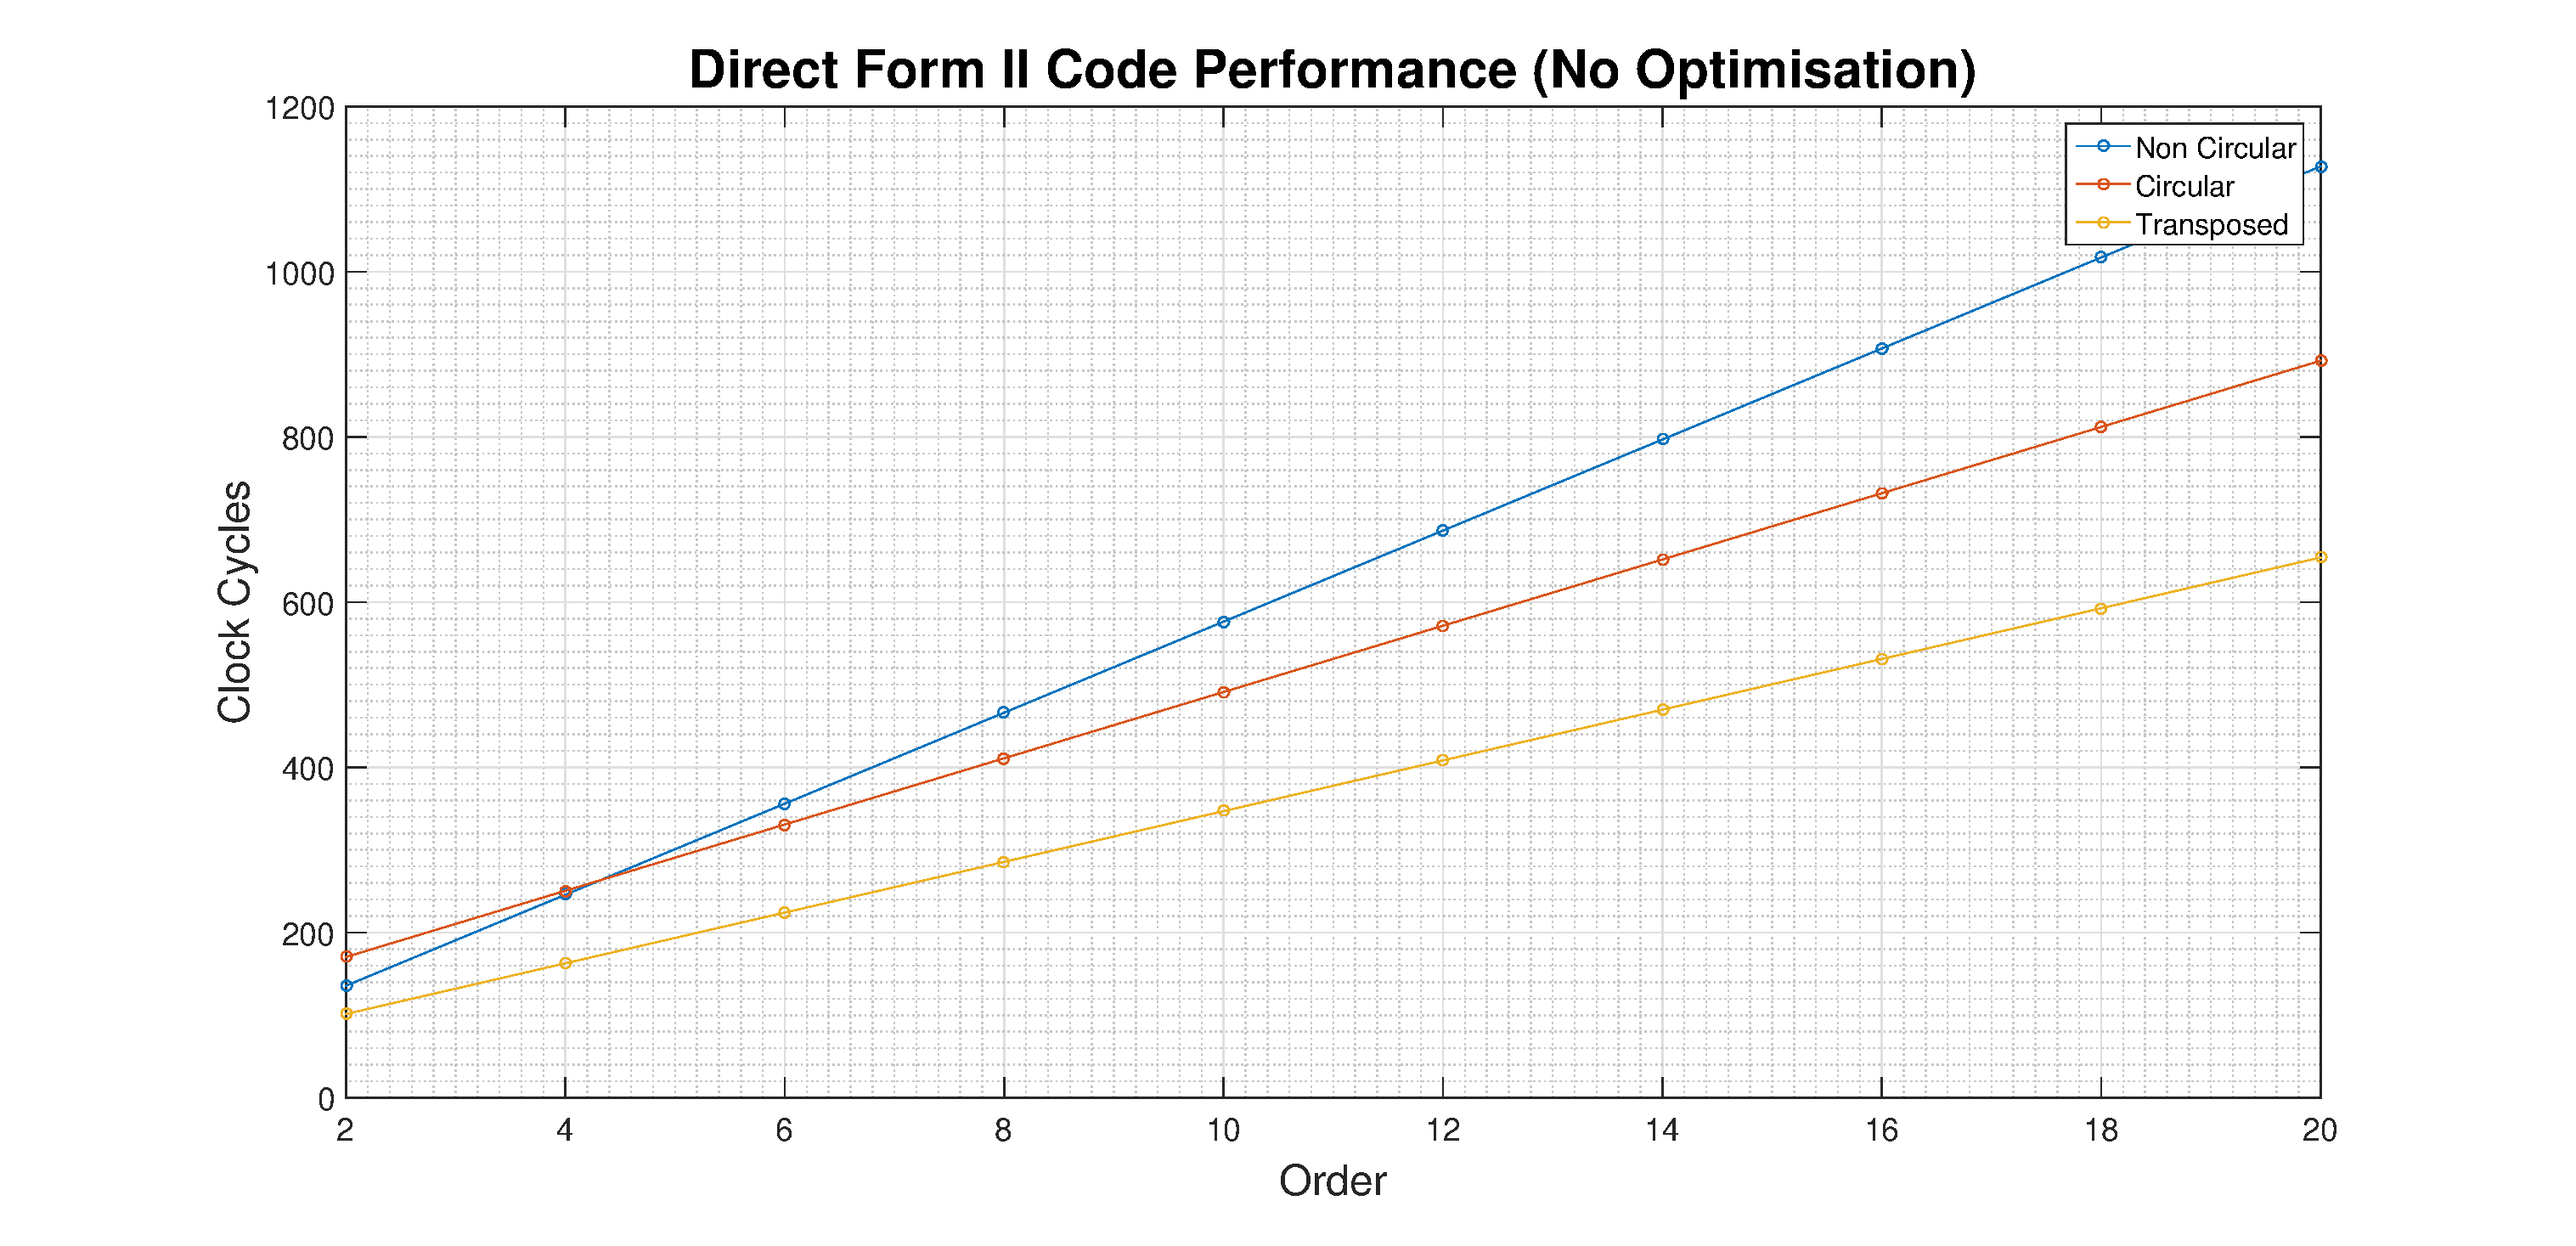
\includegraphics[width = 0.70\textwidth]{no_opt_all}
    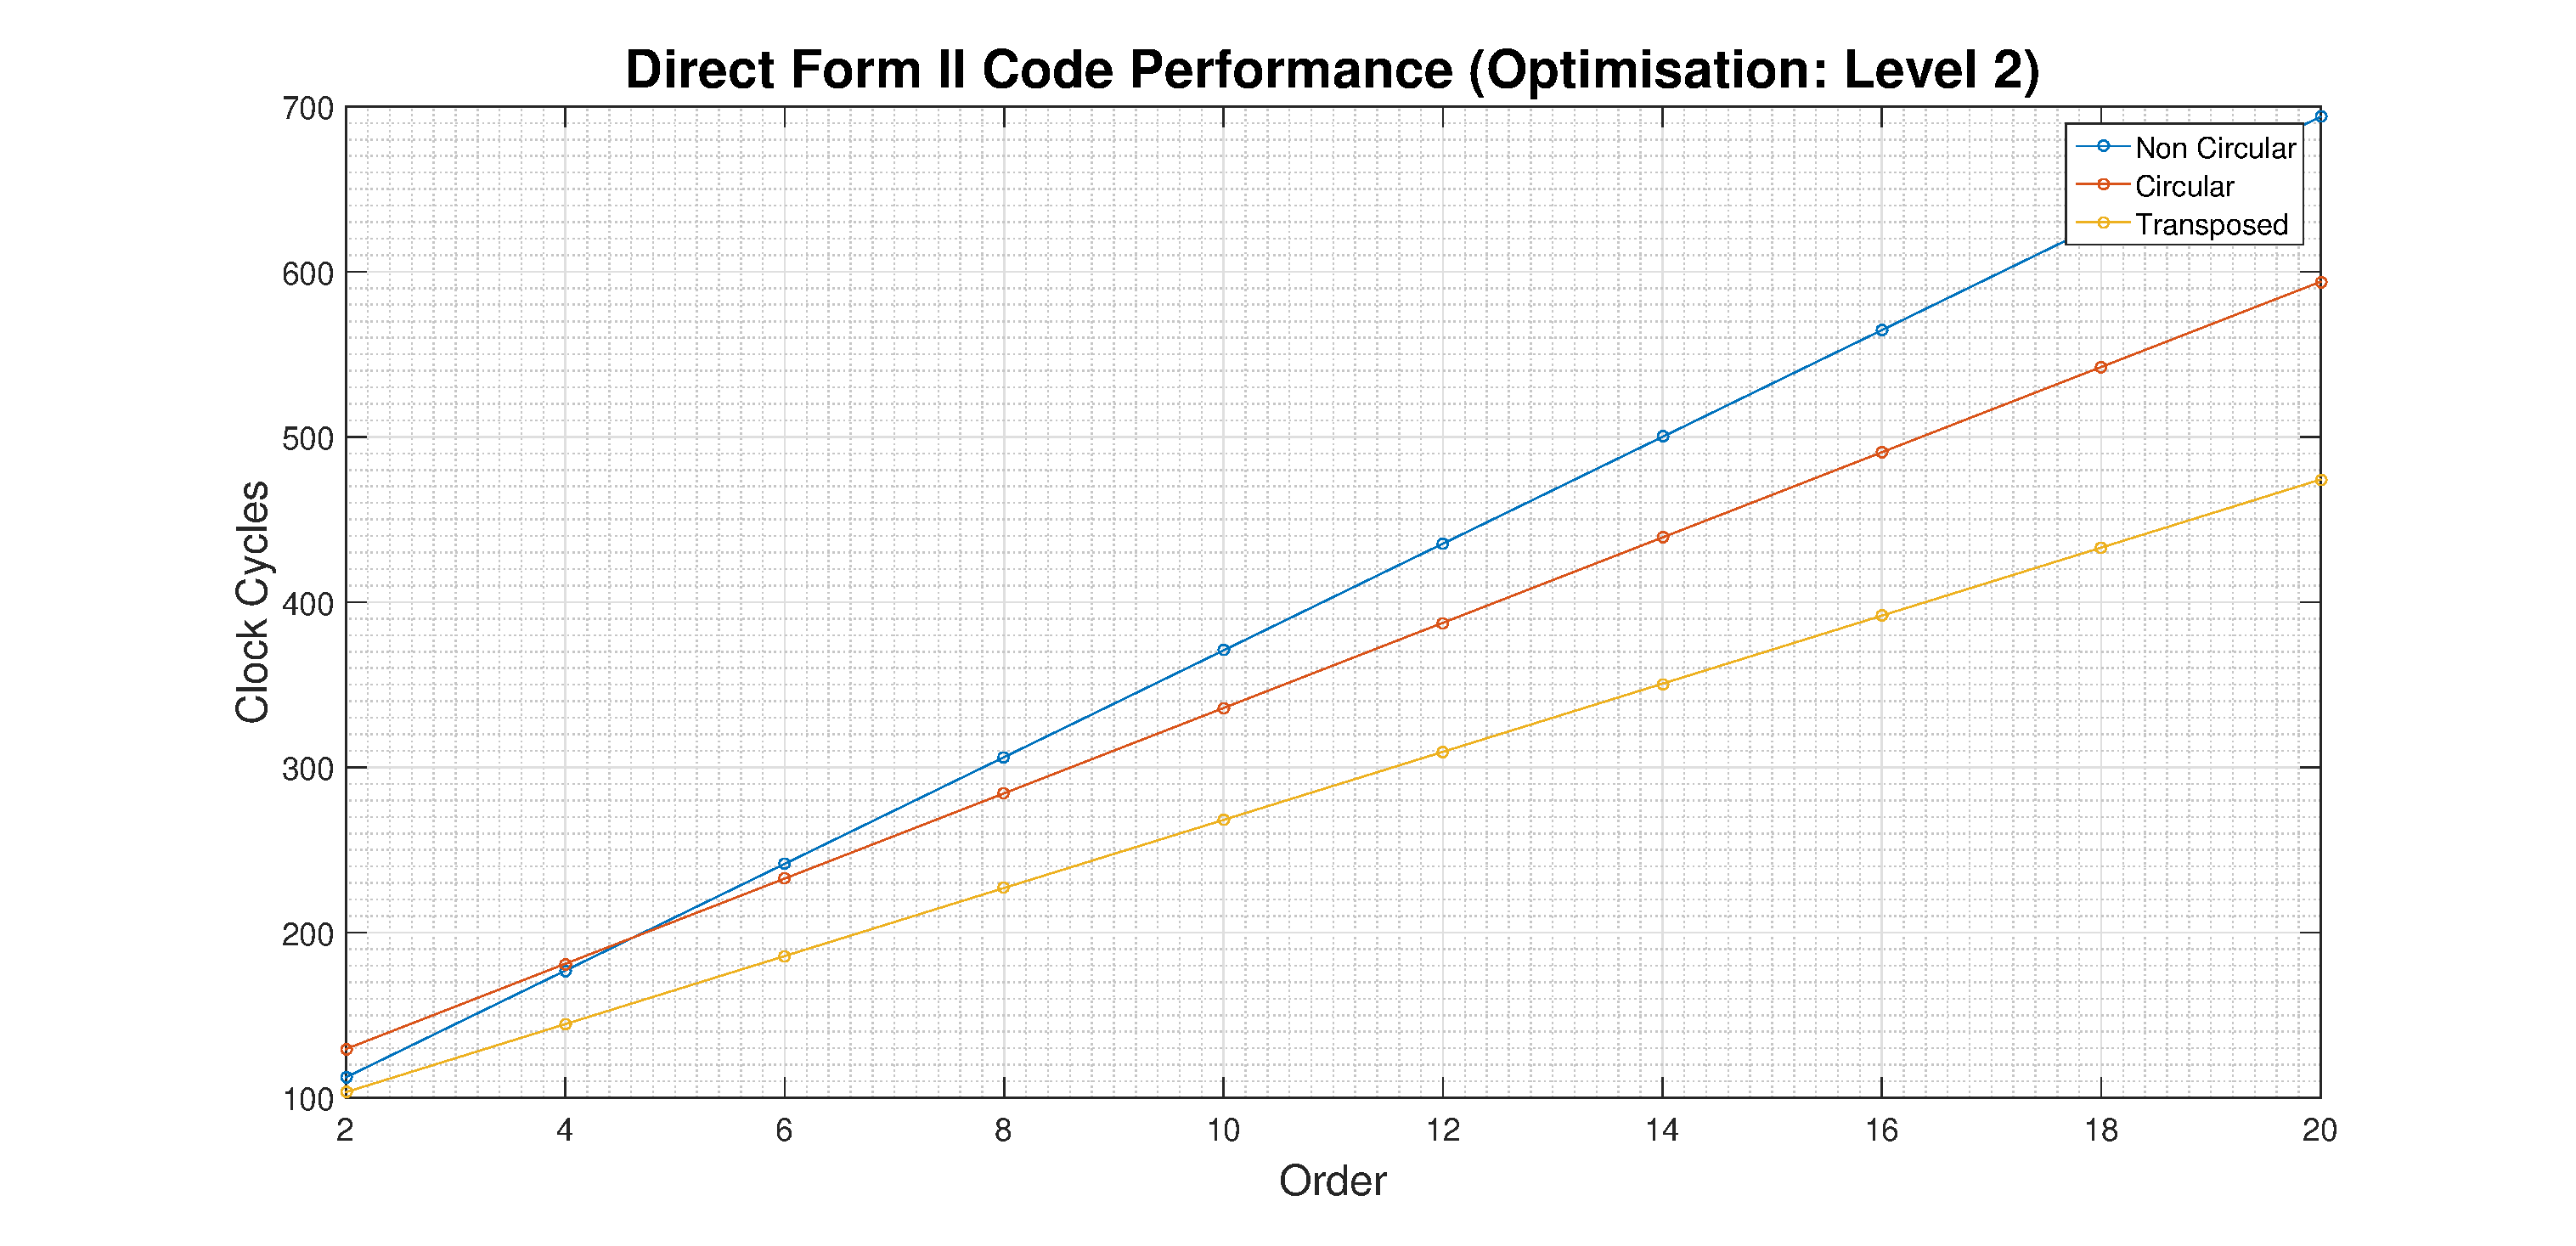
\includegraphics[width = 0.70\textwidth]{opt_all}
    \caption{Comparison of direct form II and transposed form realisations of bandpass IIR filter}
    \label{fig:compare}
\end{figure}


Finally, figure \ref{fig:compare} shows how the direct form II and transposed form compare with one another. \textbf{It is clear that the transposed form realisation performs significantly better than both implementations of the direct form II realisation.} When optimisation is used, the gradients change slightly, however the general trend remains consistent.\\

The results obtained are exactly as expected. The transposed form is expected to perform better than the direct form II realisation because of the way the buffer is implemented. The direct form II uses a buffer that stores previous input samples. To keep track of the relative delay between the current sample and past samples requires overhead in terms of computational complexity. The simple buffer keeps track of the relative delay by complete reorganisation of the buffer each time a new sample is read. The circular buffer keeps track of relative delays by changing the position of the pointer such that it points to the newest sample in the buffer.\\

The transposed form removes this overhead. The buffer in the transform form implementation keeps track of intermediate values. The buffer is overwritten by new values rather than being shifted around. This is clearly simpler to implement as noted in listing \ref{lst:transposed_form}; only 1 line of code is required within the {\tt for} loop. \\ 

\textbf{Having a smart buffer, like the one used to implement the transposed form, is quintessential. Memory access operations are very expensive and smart buffers significantly reduce the number of memory accesses.} \\

\textbf{In addition, the code composer environment is able to significantly speed up code that make use of the {\tt const} keyword. In the transposed form, the input sample and the calculated output, both required for each iteration of the {\tt for} loop, are declared as constants; their value does not change during the function call.} This again helps to speed up the performance of the code. This is not possible with the direct form II implementation 

\section{Frequency Spectrum Analysis of the Bandpass Filter}
As in section \ref{sec:RC_freq}, for accurate analysis of the bandpass filter's frequency response, it is important to remove the offset introduced by the $DSK$ board. Figure \ref{fig:bandpass_freq} shows the frequency response of the bandpass filter. The frequency response of the $4^{th}$ order filter is graphed. \textbf{Note that the frequency response for the direct form and the transposed form is equivalent. This is as expected as the two implementations might have slightly different mathematical equations, but they implement the same filter and thus produce identical outputs.}

\begin{figure}[H]
    \centering
    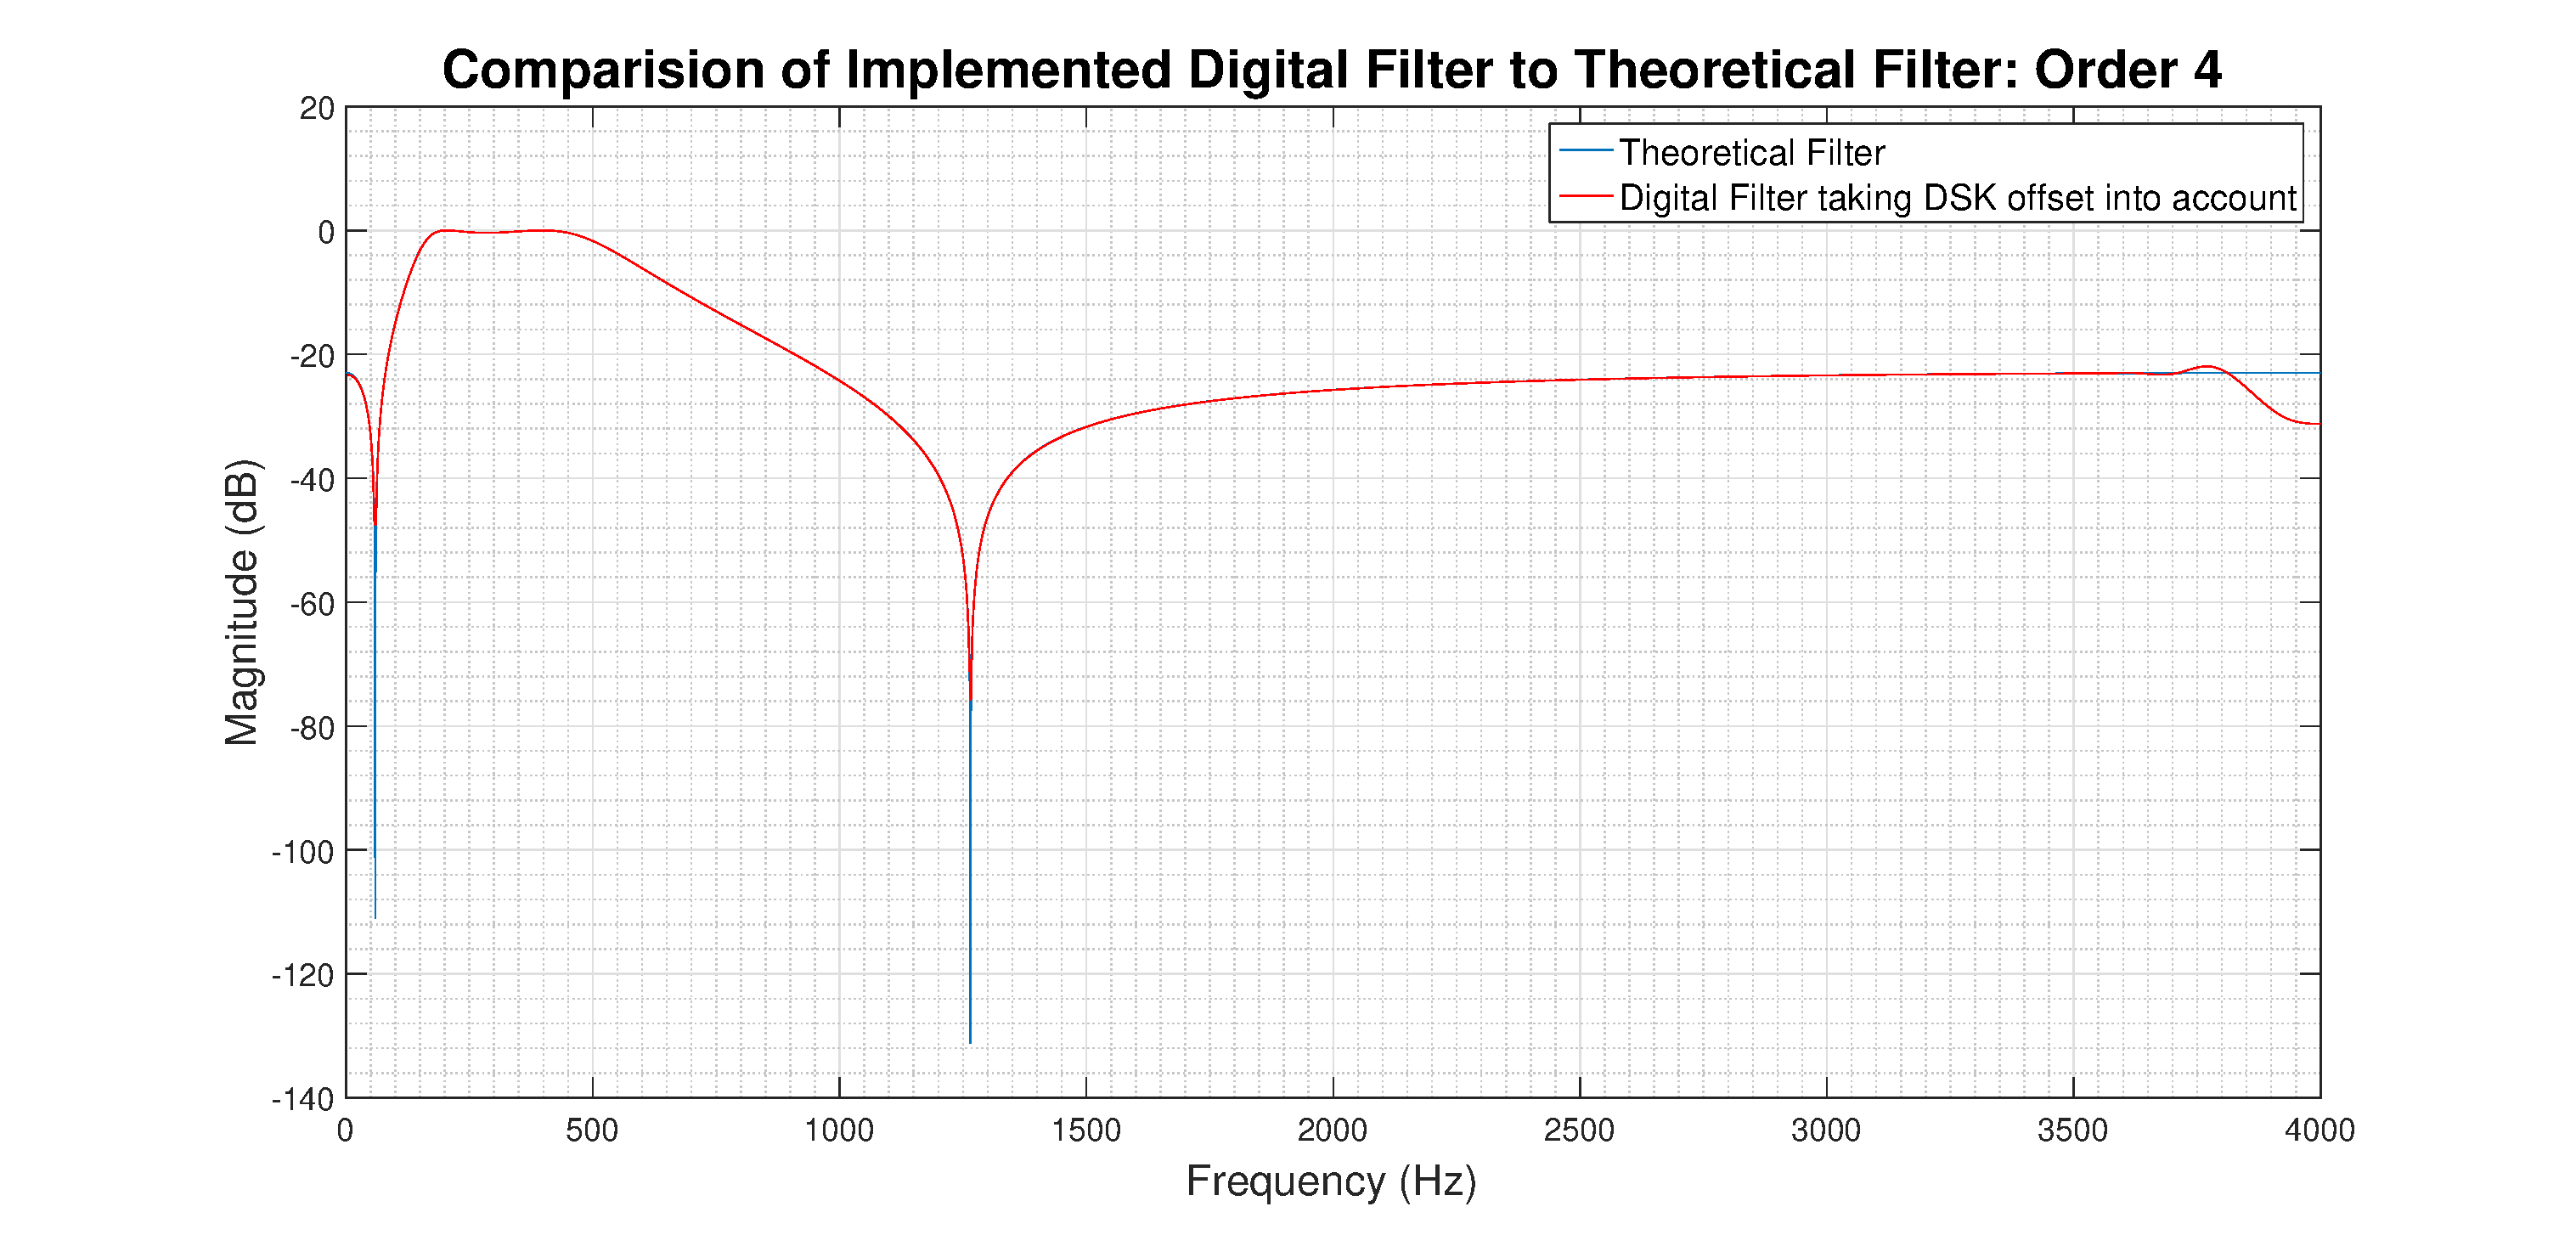
\includegraphics[width = 0.70\textwidth]{band_pass_mag_compare}
    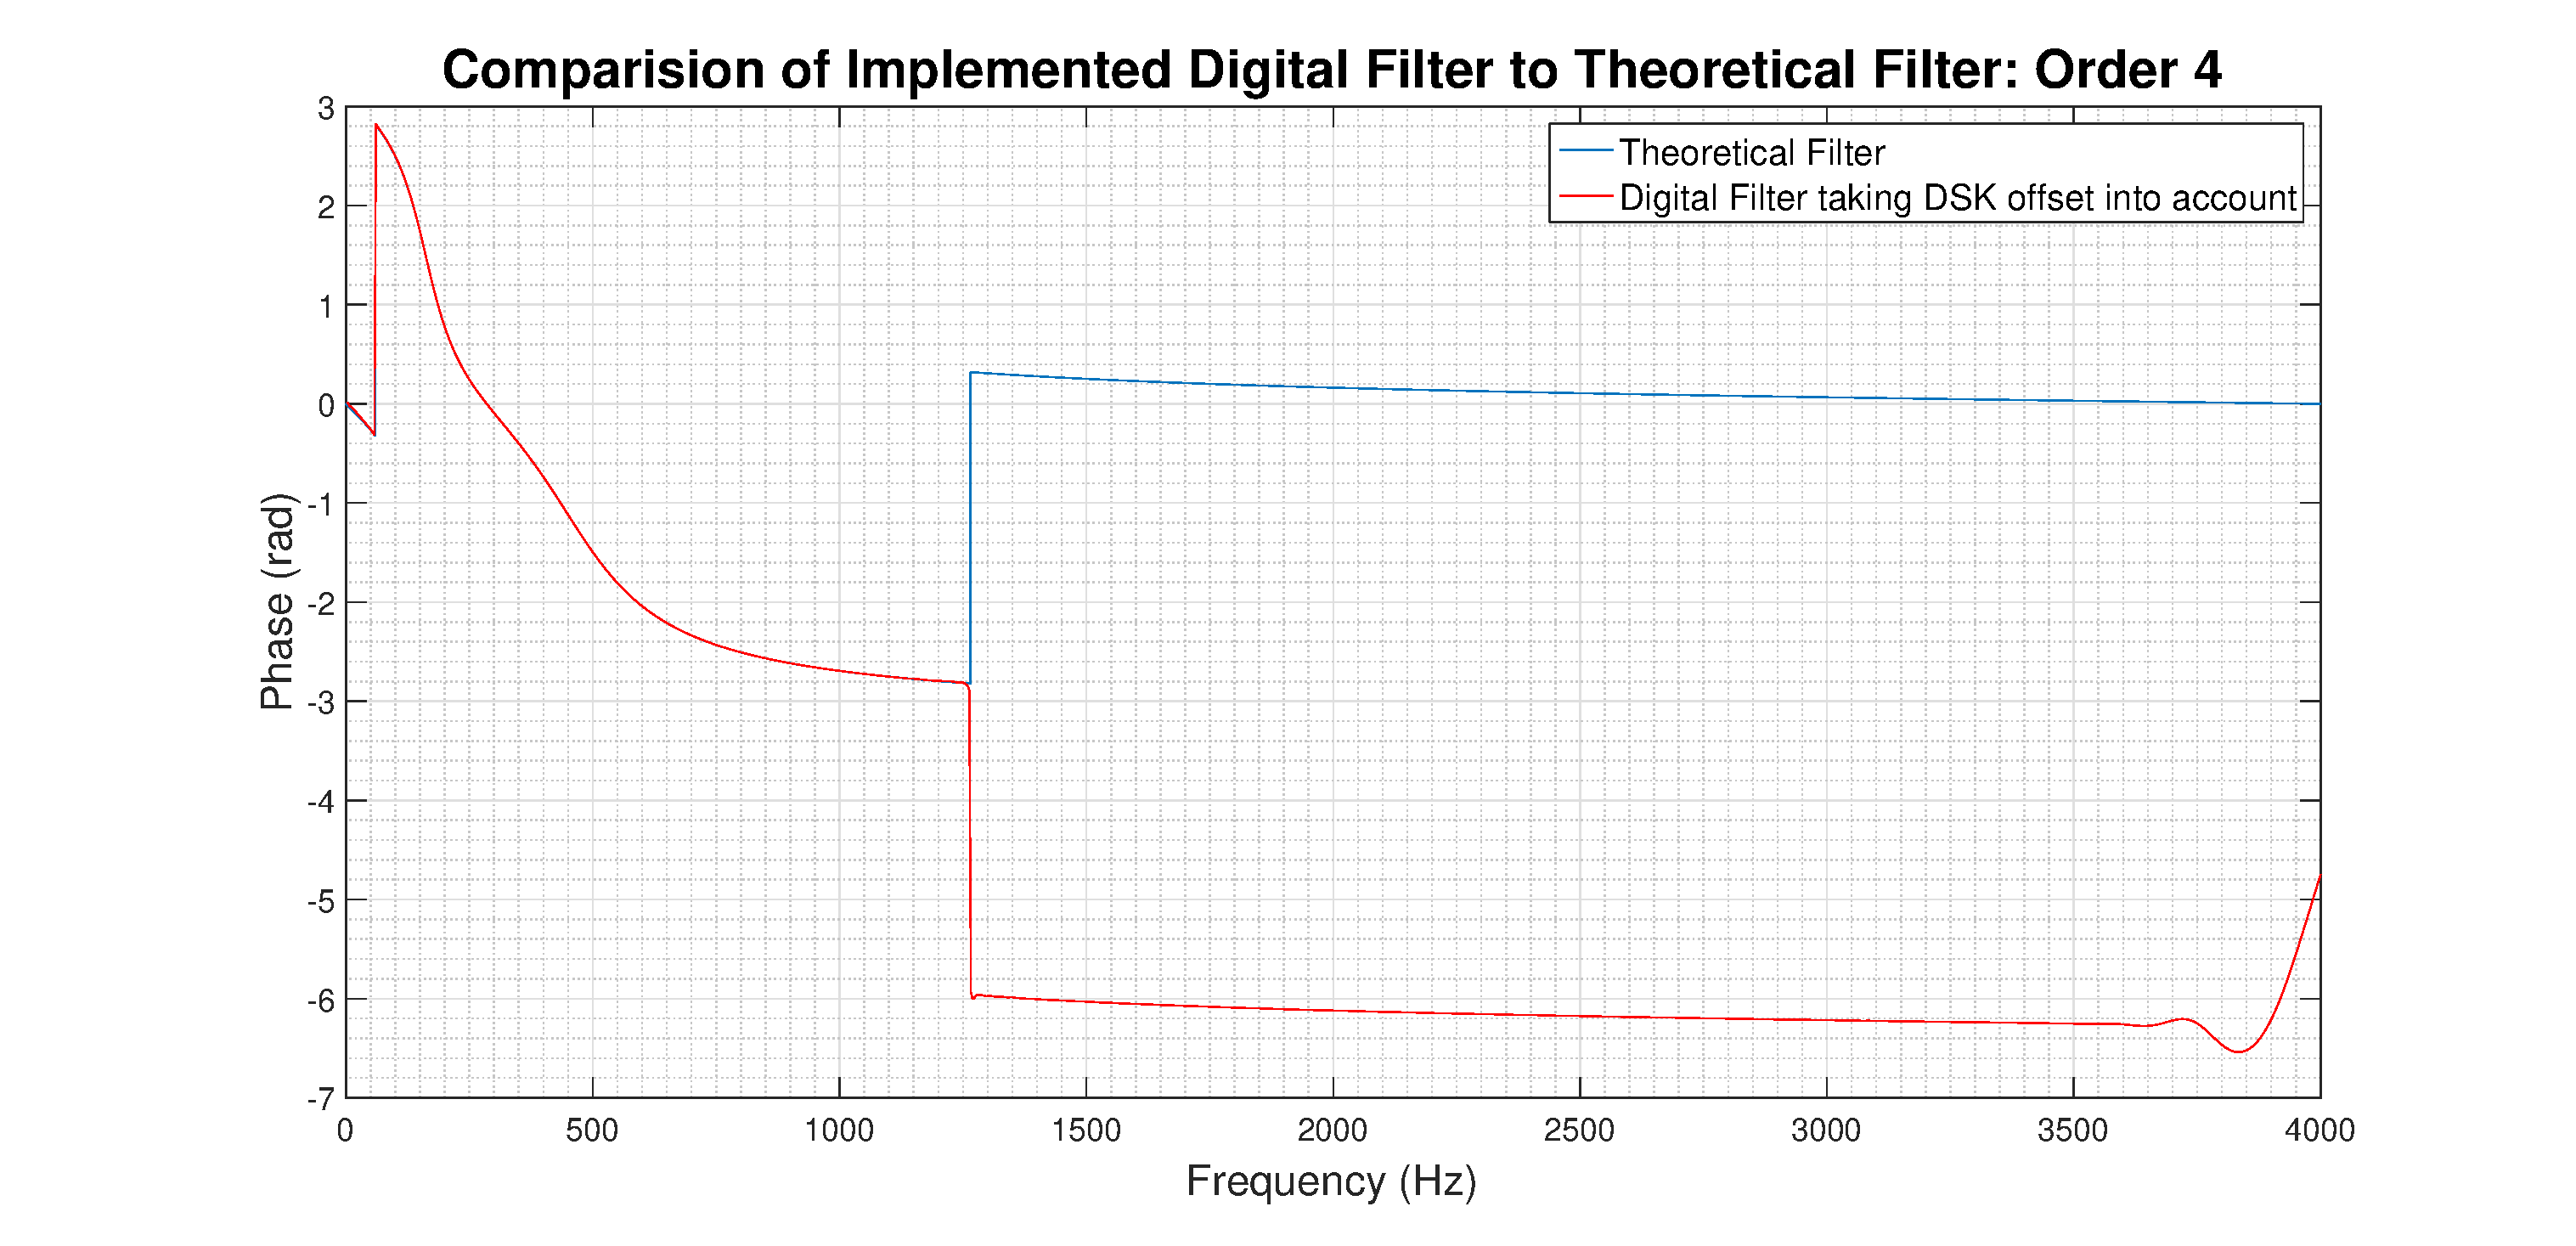
\includegraphics[width = 0.70\textwidth]{band_pass_phase_compare}
    \caption{Comparison of theoretical response and response of digital filter on $DSK$ board}
    \label{fig:bandpass_freq}
\end{figure}

 Superimposed on the graphs are the original filter response that was designed on MATLAB. Figure \ref{fig:bandpass_freq} confirms that the filter correctly implements the filtering process that it was designed for. It meets all the specifications that were set out in the laboratory 5 script.\textbf{ Note the discrepancy in the phase comes from the way that the phase is unwrapped and does not mean that the filter is not performing as expected. Near $4kHz$, both magnitude and phase response diverge slightly from the ideal response due to the anti-aliasing filter.}
 
\section{Stability of Elliptic Filter}

\textbf{The method used to design the elliptic filter on MATLAB should theoretically produce stable filters. However due to finite memory constraints, the filter coefficients incur rounding errors. This causes poles and zeros to drift away from their actual position on the z-plane.}\\

In MATLAB there are two methods of using the {\tt ellip} function to design a filter: \begin{itemize}
    \item Producing filter coefficients
    \item Producing poles and zeros
\end{itemize} 
\textbf{Since the filtering process is going to be implemented in the time domain using multiply accumulate operations, filter coefficients are produced.} This method of filter design is referred to as the Transfer Function (TF) design methodology. In contrast, the Zero-Pole-Gain (ZPK) design method\footnote{This design methodology is referred to as the ZPK method, where K is used to signify gain.} produces the position of poles and zeros on the complex plane. The ZPK method is less susceptible to the drifting of poles and zeros as it is less sensitive to finite precision effects. The ZPK design method uses a biquad implementation as opposed to the direct form I/II implementation of the filter. See Appendix A for the filter co-efficients that MATLAB uses for the TF and ZPK design (for N = 14). 


\begin{figure}[H]
    \centering
    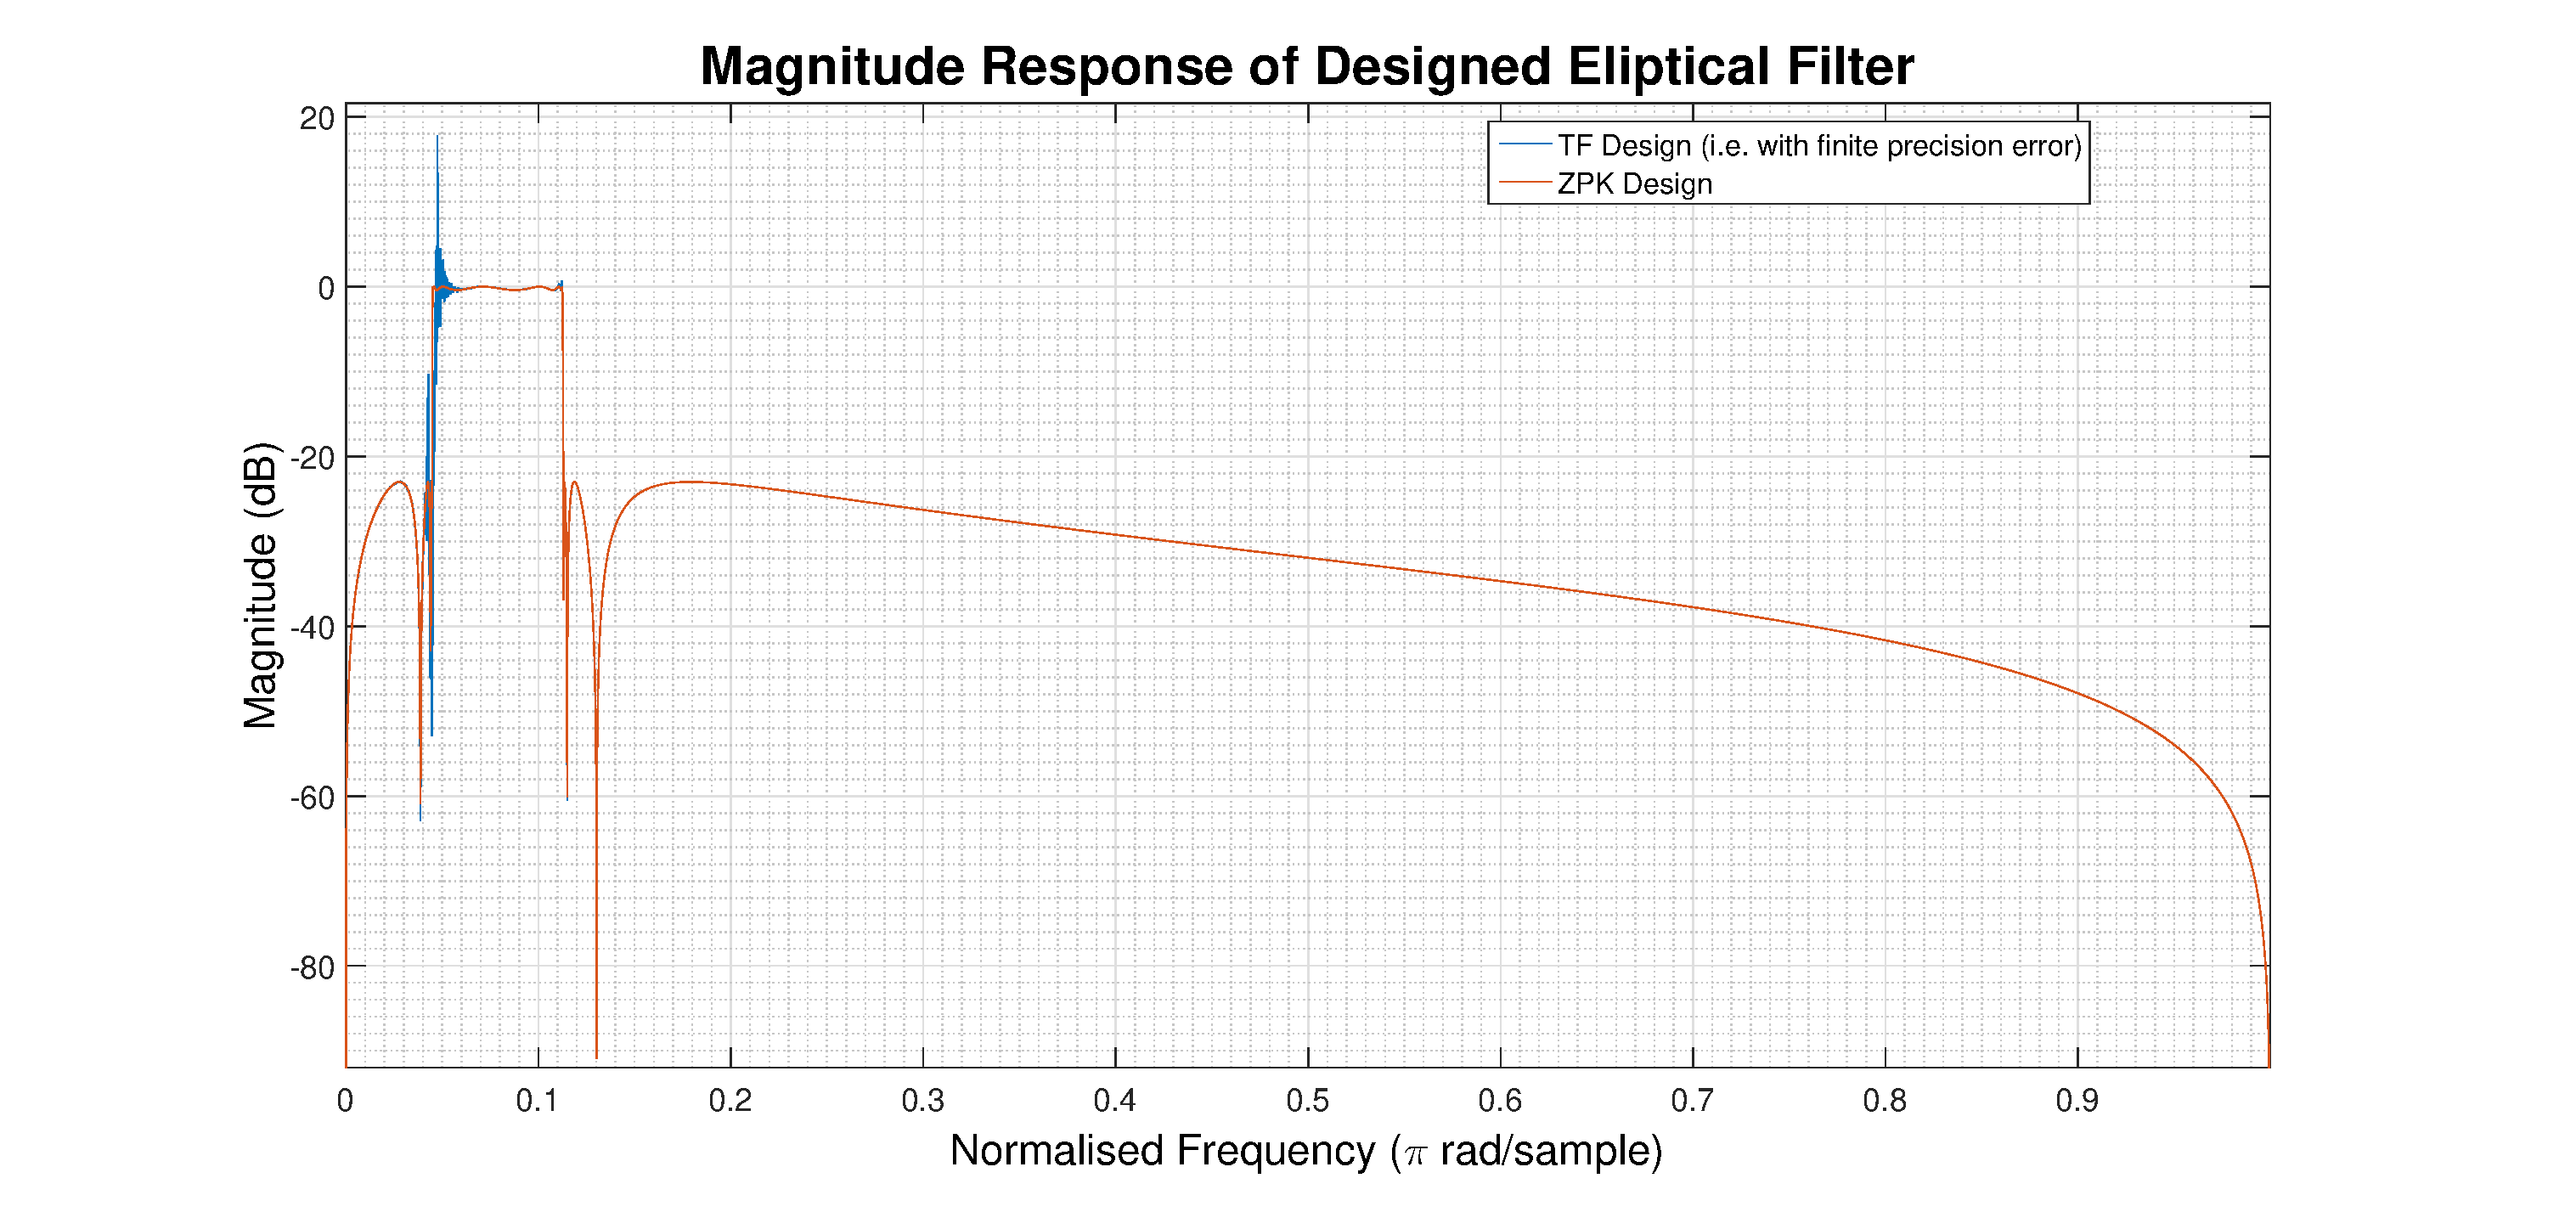
\includegraphics[width = 0.70\textwidth]{moniri_2}
    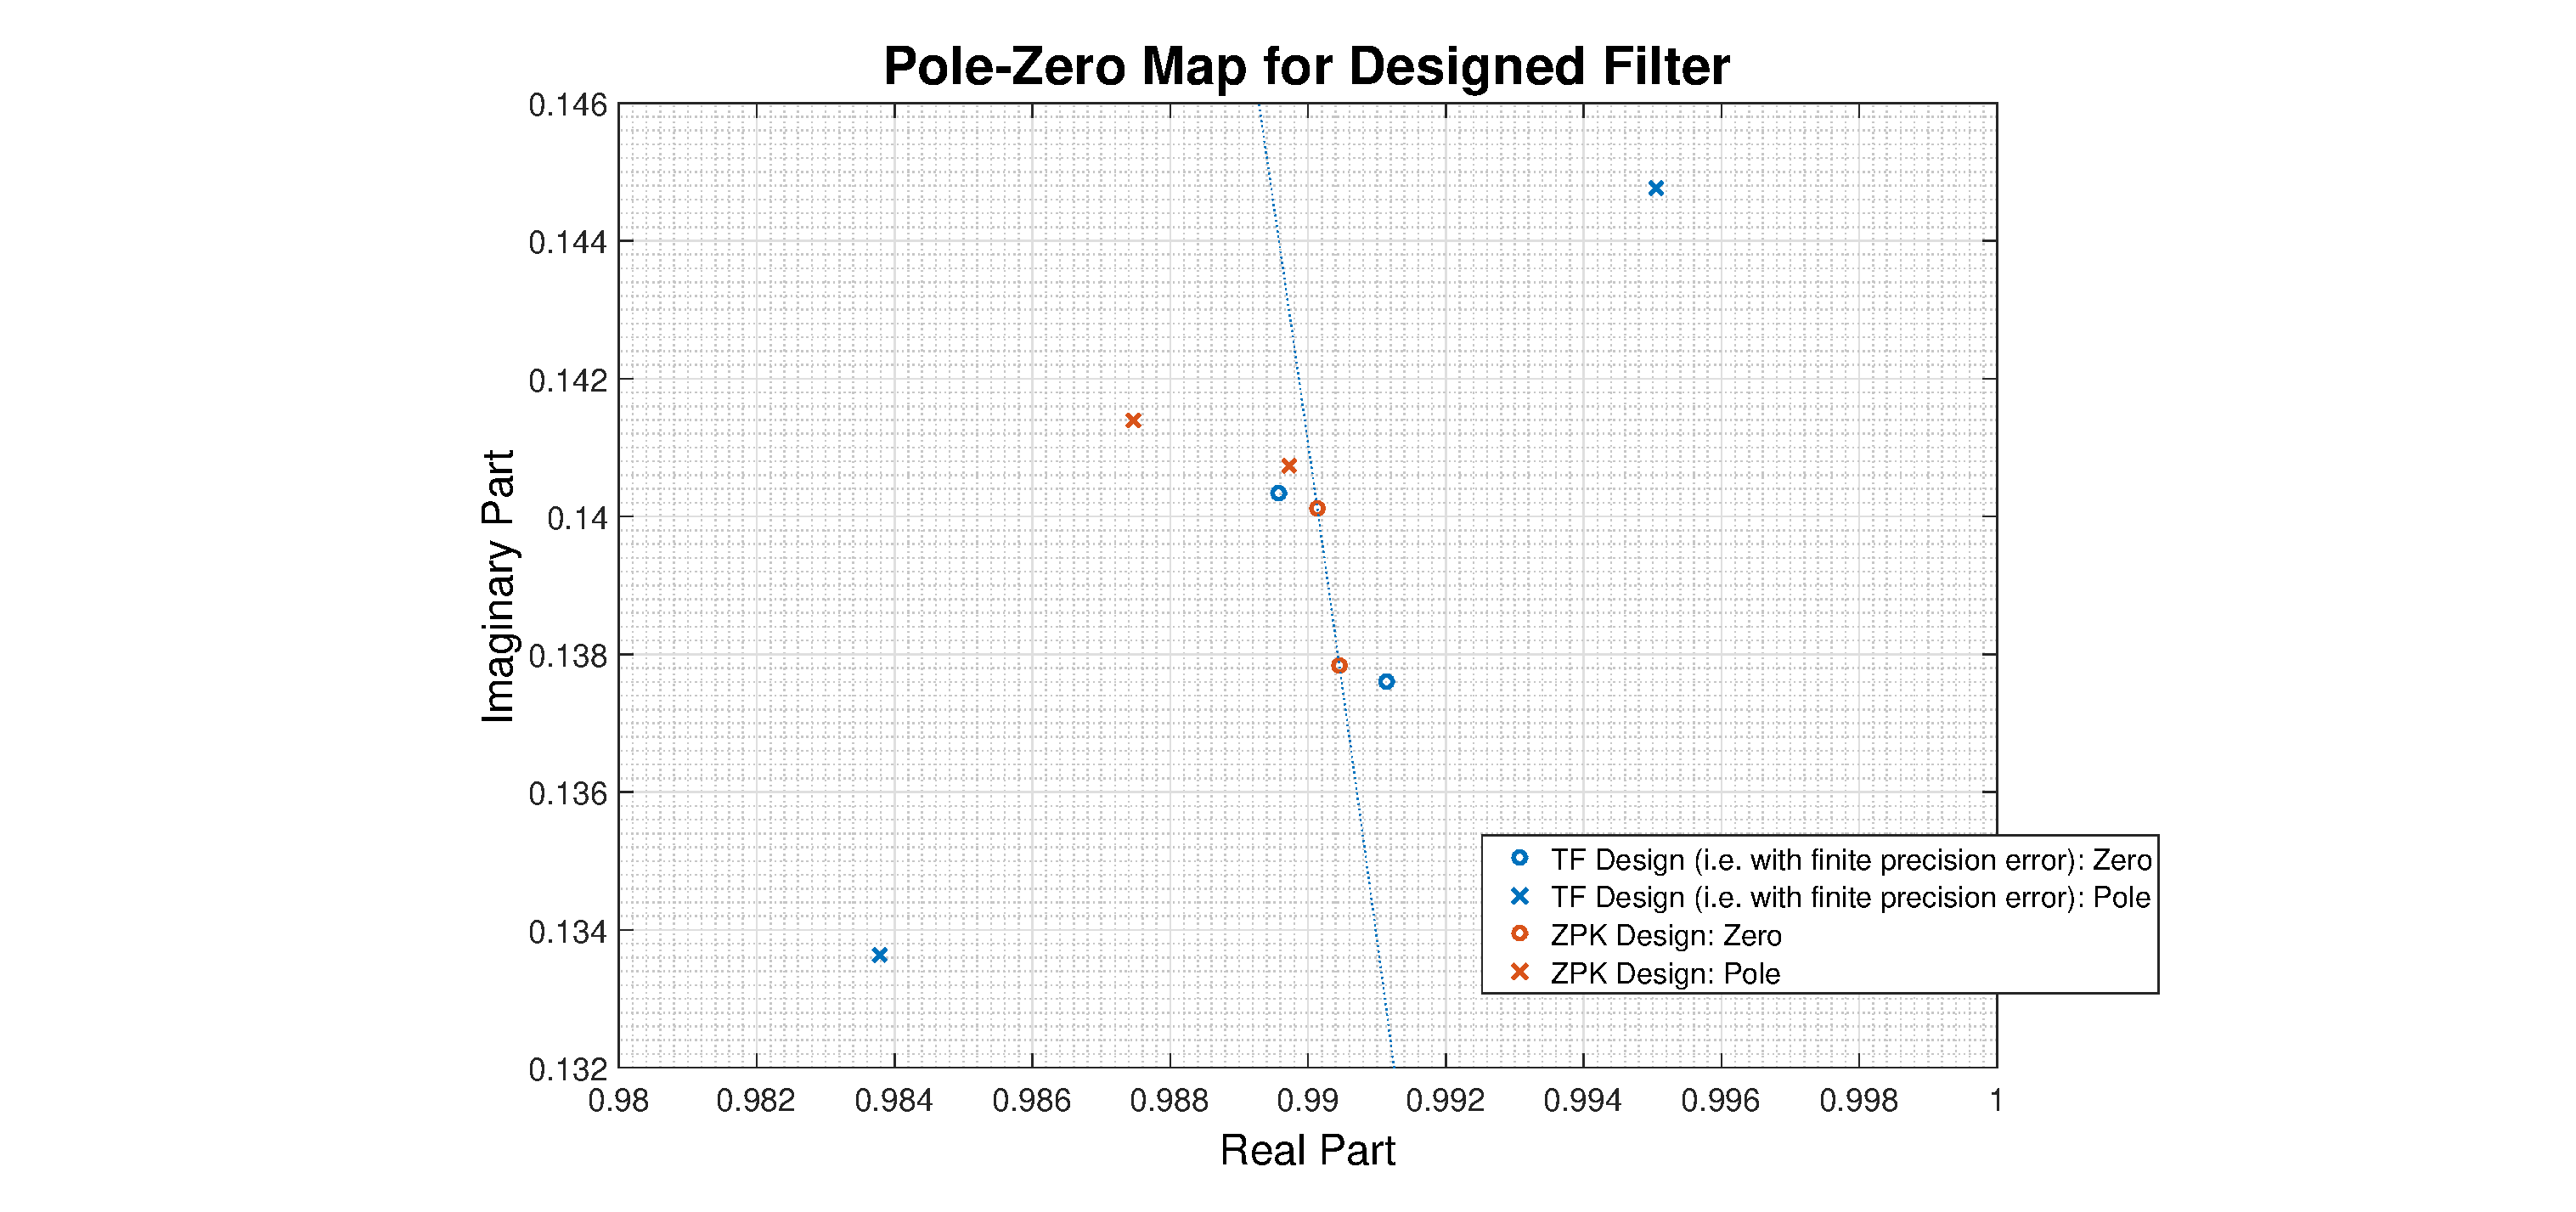
\includegraphics[width = 0.70\textwidth]{moniri_1}
    \caption{}
    \label{fig:moniri}
\end{figure}


\textbf{While increasing the order of the bandpass elliptical filter, it was observed that at N = 14, the filter became unstable.} Figure \ref{fig:moniri} shows the magnitude response of the TF design and the \textit{ideal} ZPK design. The difference in frequency response is clear. \textbf{The pole-zero plot shows that a pole has drifted out of the unit circle when the TF methodology was used.}\\

In the design of IIR filters such as elliptic filters, poles placed near the edge of the unit circle, when high-order filters are designed, may drift out of the unit circle due to finite precision effects; the resulting filter will become unstable.

\section{Conclusion}
This report presented the theory behind IIR filters and the discussed generation of filters using the MATLAB functions. A detailed discussion about implementing IIR filters on the $TMS320C6713 \ DSK$ board is presented. Compiler optimisations and different filter realisations were considered. Lastly the frequency spectrum of the designed filter was observed. The designed filter met all specifications listed in laboratory 5. It was noted that for filter of high orders, instability might occur. The reasons for instability were discussed and an alternative design methodology was explored. 

\begin{thebibliography}{99}
\bibitem{AIC23_technical_reference} Instruments, T. (2004). TLV320AIC23B, Stereo Audio CODEC, Data Manual. Retrieved February 04, 2016, from \url{http://www.ti.com/lit/ds/symlink/tlv320aic23b.pdf}
\end{thebibliography}

\newpage
\appendix
\section{Comparison of TF and ZPK Design Methodologies}
\begin{listing}[H]
\begin{minted}[fontsize=\scriptsize,linenos]{MATLAB}
fsamp = 8000;                   % defines the sampling frequency
order = 4;                      % defines the order of the digital filter
passband_ripple = 0.4;          % defines the passband ripple
stopband_attenuation = 23;      % defines the stopband attenuation of the filter
Wp = [180 450]/(0.5*fsamp);     % normalising edge frequencies of passband


% ellip function designs filter of order 2n
[b, a] = ellip(order/2, passband_ripple, stopband_ripple, Wp, 'bandpass');

% Zero-Pole-Gain design
[z,p,k] = ellip(order/2, passband_ripple, stopband_ripple, Wp, 'bandpass');
sos = zp2sos(z,p,k);
\end{minted}
\caption{MATLAB code to compare TF and ZPK design methodologies} 
\label{lst:MATLAB_elliptical}
\end{listing}


\begin{figure}[H]
    \centering
    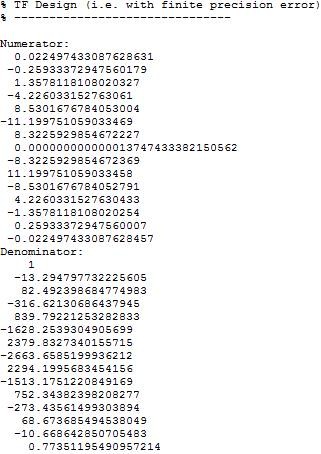
\includegraphics[width = 0.49\textwidth]{biquad_2}
    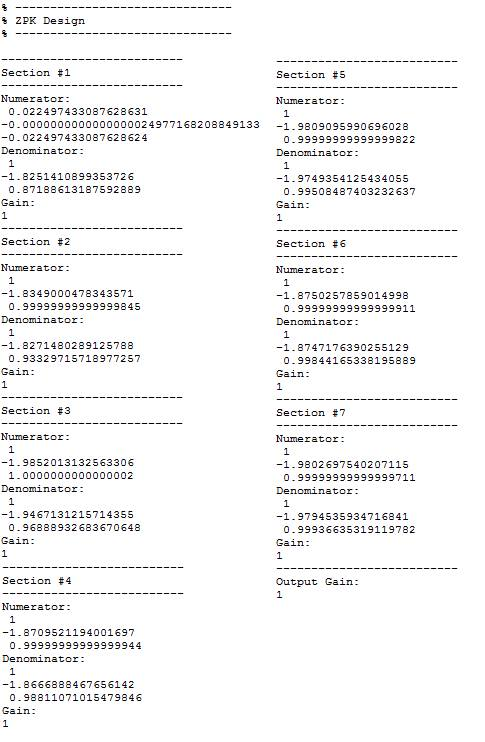
\includegraphics[width = 0.49\textwidth]{biquad_1}
    \caption{Comparison of TF and ZPK filter design methodologies}
    \label{fig:my_label}
\end{figure}
\end{document}




